% -*- TeX-master: "sbml-level-2-version-3"; fill-column: 66 -*-
% $Id$
% $Source$
% ----------------------------------------------------------------

\section{SBML components}
\label{sec:elements}

\begin{blockChanged}

In this section, we define each of the major components of SBML.
We use the UML notation described in
Section~\ref{sec:notation-uml} for defining classes of objects.
We also illustrate the use of SBML components by giving partial
model definitions in XML.  Section~\ref{sec:xml-rep} provides many
full examples of SBML in XML.

\end{blockChanged}


%-----------------------------------------------------------------------------
\subsection{The SBML container}
\label{sec:sbml}
%-----------------------------------------------------------------------------

\begin{blockChanged}

All well-formed XML documents must begin with an \emph{XML
  declaration}, which specifies both the version of XML assumed
and the document character encoding.  The declaration begins with
the characters \token{<?xml} followed by the XML \token{version}
and \token{encoding} attributes.  \sbmltwo uses XML version 1.0
and requires a document encoding of UTF-8.  Following this XML
declaration, the outermost portion of a model expressed in SBML
\changed{\thisLV} consists of an object of class \Sbml, defined in
Figure~\ref{fig:sbml}.  This class contains two required
attributes, for the SBML \token{level} and \token{version}, and
one required subelement called \token{model} whose class is
\Model.

\begin{figure}[htb]
  \centering
  \small
  \vspace*{-2ex}
  \begin{tikzpicture}[level distance=0.85in]
    \node { \emptyClassbox{\textsl{SBase}} }
      [open triangle 60-,edge from parent fork down,sibling distance=2.65in]
      child {node (a) {
          \begin{classbox}{Sbml}
            xmlns: string \{ "http://www.sbml.org/sbml/level2/version3" \} \\
            level: positiveInteger \{ use="required" fixed="2" \}   \\
            version: positiveInteger \{ use="required" fixed="\changed{3}" \} \\
          \end{classbox}
        }}
      child {node (b) {
          \emptyClassbox{Model}
        }}
     ;
     \draw[diamond-] (a) -- (b) 
       node[above=6pt,left=45pt] {\textsf{model}};
  \end{tikzpicture}
  \caption{\changed{The definition of \Sbml for \sbmltwothree.
      The class \Model is defined in Section~\ref{sec:model}.
      Note that both \Sbml and \Model are subclasses of \SBase,
      and therefore inherit the attributes of that abstract
      class.}}
  \label{fig:sbml}
\end{figure}

The following is an abbreviated example of these XML elements for
an \sbmltwothree document:

\end{blockChanged}

\begin{example}
<?xml version="1.0" encoding="UTF-8"?>
<sbml xmlns="http://www.sbml.org/sbml/level2/\changed{version3}" level="2" version="\changed{3}">
  ...
</sbml>
\end{example}

The attribute \token{xmlns} declares the default XML namespace
used within the \token{sbml} element.  The URI for SBML Level~2 Version~\changed{3}
is \uri{http://www.sbml.org/sbml/level2/\changed{version3}}.  All
elements must be placed in this namespace either by assigning the
default namespace as shown above, or using a tag prefix on
every element.

An SBML XML document must not contain elements or attributes in
the SBML namespace that are not defined in this SBML \changed{\thisLVR}
specification.  Documents containing unknown elements or
attributes placed in the SBML namespace do not conform to \changed{this
SBML} specification.

Readers may wonder why the SBML top-level XML element uses both a
namespace URI identifying the SBML level and version, as well as
separate XML attributes giving the level and version.  Why is the
information duplicated?  There are several reasons.  First, XML is
only one possible serialization of SBML (albeit an extremely
popular one at this time).  Though most of this document is
written with XML in mind, it is the intention behind the design of
SBML that its object structure should be implementable in other
languages and software systems.  Programmatic access is easier if
the level and version information are accessible directly as data
rather than have to be extracted from a string.  Second, generic
high-level XML parsers may not give their calling programs access
to the value of the \texttt{xmlns} attribute.  Providing the
information via separate attributes is a good backup measure.  And
finally, earlier in the history of SBML, it was expected that only
the level needed to be encoded as part of the namespace URI (e.g.,
\uri{http://www.sbml.org/sbml/level1}) because it was hoped that
changes within levels would not require XML Schema changes.  This
has proven to be false, but SBML Level~1 (both versions) and the
first version of SBML Level~2 still subscribe to this principle.
This means that for these variants of SBML, software tools must
look for a \token{version} attribute on the top-level element.
For backwards compatibility with software that expects this, it
makes more sense to keep the version and level attributes.


%-----------------------------------------------------------------------------
\subsection{Model}
\label{sec:model}
%-----------------------------------------------------------------------------

\begin{blockChanged}

The definition of \Model is shown in Figure~\vref{fig:model}.
Only one instance of a \Model object is allowed per instance of an
SBML \thisLVR document or data stream, and it must be located
inside the \token{<sbml> ...\ </sbml>} element as described in
Section~\ref{sec:sbml}.

\begin{figure}[htb]
  \centering
  \vspace*{-2ex}
  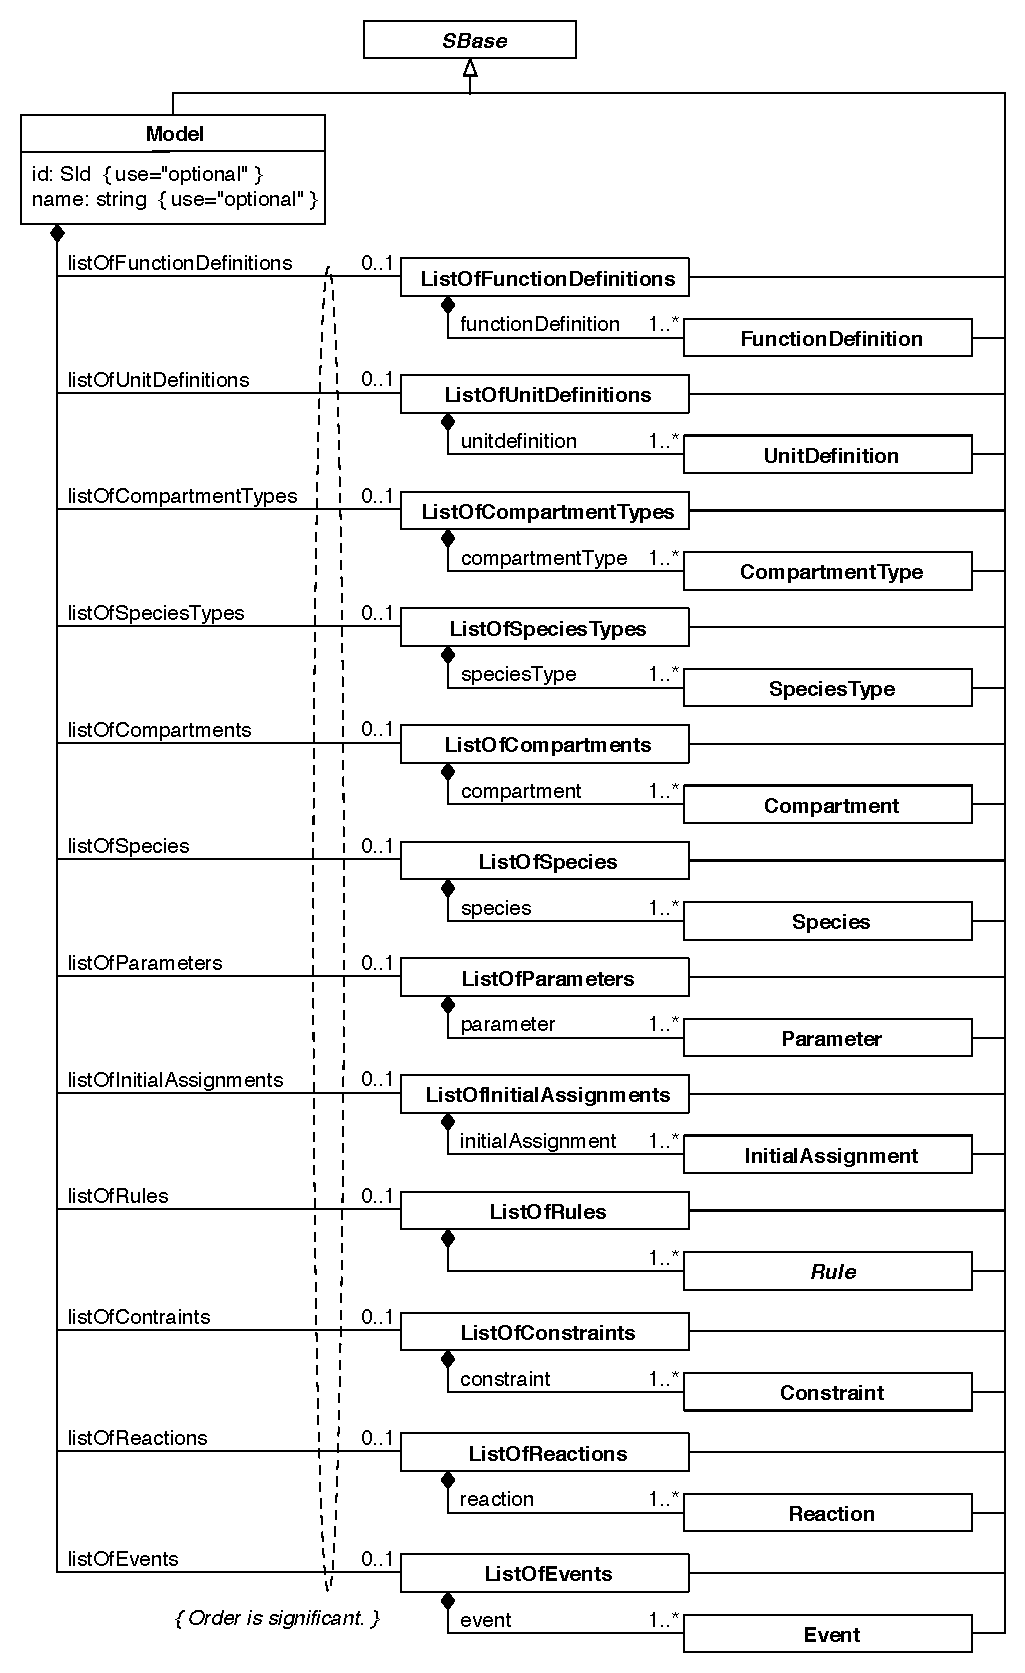
\includegraphics[scale=0.755]{figs/model-uml}
  \caption{\changed{The definition of \Model and the helper
      classes \ListOfFunctionDefinitions, \ListOfUnitDefinitions,
      \ListOfCompartmentTypes, \ListOfSpeciesTypes,
      \ListOfCompartments, \ListOfSpecies, \ListOfParameters,
      \ListOfInitialAssignments, \ListOfRules, \ListOfConstraints,
      \ListOfReactions, and \ListOfEvents.}}
  \label{fig:model}
\end{figure}

The \Model \changed{object} has an optional \changed{attribute}, \token{id}, used to
give the model an identifier.  The identifier must be a text
string conforming to the syntax permitted by the \primtype{SId}
data type described in Section~\ref{sec:sid}.  \Model also has an
optional \token{name} \changed{attribute}, of type \primtype{string}.  The
\token{name} and \token{id} \changed{attributes} must be used as described in
Section~\ref{sec:idnameattribs}.

\Model serves as a container for components of classes
\FunctionDefinition, \UnitDefinition, \CompartmentType,
\SpeciesType, \Compartment, \Species, \Parameter,
\InitialAssignment, \Rule, \Constraint, \Reaction and \Event.
Instances of the classes are placed inside instances of classes
\ListOfFunctionDefinitions, \ListOfUnitDefinitions,
\ListOfCompartmentTypes, \ListOfSpeciesTypes, \ListOfCompartments,
\ListOfSpecies, \ListOfParameters, \ListOfInitialAssignments,
\ListOfRules, \ListOfConstraints, \ListOfReactions, and
\ListOfEvents.  The ``list'' classes are defined in
Figure~\ref{fig:model}.  All of the lists are optional, but if a
given list container is present within the model, the list must
not be empty; that is, it must have length one or more.  The
resulting XML data object for a full model containing every
possible list would have the following form:

\newcommand{\sayOptional}{\raisebox{0pt}[0pt][0pt]{\bigg\} \textrm{\emph{optional}}}}

\vspace*{1.5ex}
\begin{tt}
  \tightspacing
  \small
  \begin{tabbing}
xxxx\=xxxx\=xxxx\=xxxx\=xxxx\=\kill
\+\>
<?xml version="1.0" encoding="UTF-8"?>\\
<sbml xmlns="http://www.sbml.org/sbml/level2/\changed{version3}" level="2" version="\changed{3}">\\
\><model id="My\_Model">\\
\>\><listOfFunctionDefinitions>\\
\>\>\>\textrm{\emph{one or more}} <functionDefinition> ... </functionDefinition> \textrm{\emph{elements}}  \` \sayOptional\\
\>\></listOfFunctionDefinitions>\\
\>\><listOfUnitDefinitions>\\
\>\>\>\textrm{\emph{one or more}} <unitDefinition> ... </unitDefinition> \textrm{\emph{elements}}  \` \sayOptional\\
\>\></listOfUnitDefinitions>\\
\>\><listOfCompartmentTypes>\\
\>\>\>\textrm{\emph{one or more}} <compartmentType> ... </compartmentType> \textrm{\emph{elements}}  \` \sayOptional\\
\>\></listOfCompartmentTypes>\\
\>\><listOfSpeciesTypes>\\
\>\>\>\textrm{\emph{one or more}} <speciesType> ... </speciesType> \textrm{\emph{elements}}  \` \sayOptional\\
\>\></listOfSpeciesTypes>\\
\>\><listOfCompartments>\\
\>\>\>\textrm{\emph{one or more}} <compartment> ... </compartment> \textrm{\emph{elements}}  \` \sayOptional\\
\>\></listOfCompartments>\\
\>\><listOfSpecies>\\
\>\>\>\textrm{\emph{one or more}} <species> ... </species> \textrm{\emph{elements}}  \` \sayOptional\\
\>\></listOfSpecies>\\
\>\><listOfParameters>\\
\>\>\>\textrm{\emph{one or more}} <parameter> ... </parameter> \textrm{\emph{elements}}  \` \sayOptional\\
\>\></listOfParameters>\\
\>\><listOfInitialAssignments>\\
\>\>\>\textrm{\emph{one or more}} <initialAssignment> ... </initialAssignment> \textrm{\emph{elements}}  \` \sayOptional\\
\>\></listOfInitialAssignments>\\
\>\><listOfRules>\\
\>\>\>\textrm{\emph{one or more elements of subclasses of \abstractclass{Rule}}}  \` \sayOptional\\
\>\></listOfRules>\\
\>\><listOfConstraints>\\
\>\>\>\textrm{\emph{one or more}} <constraint> ... </constraint> \textrm{\emph{elements}}  \` \sayOptional\\
\>\></listOfConstraints>\\
\>\><listOfReactions>\\
\>\>\>\textrm{\emph{one or more}} <reaction> ... </reaction> \textrm{\emph{elements}}  \` \sayOptional\\
\>\></listOfReactions>\\
\>\><listOfEvents>\\
\>\>\>\textrm{\emph{one or more}} <event> ... </event> \textrm{\emph{elements}}  \` \sayOptional\\
\>\></listOfEvents>\\
\></model>\\
</sbml>
\end{tabbing}
\regularspacing
\end{tt}
\vspace*{1ex}

Although all the lists are optional, there are dependencies
between SBML components such that defining some components
requires defining others.  An example is that defining a species
requires defining a compartment, and defining a reaction requires
defining a species.  The dependencies are explained throughout the
text.
  
% Contortion to make the section number be colored for the rest of
% this subsection.

\makeatletter
\renewcommand{\thesubsubsection}{\changed{\thesubsection .\@arabic\c@subsubsection}}
\makeatother

\subsubsection{The ListOf container classes}
\label{sec:listofunitdefinitions}
\label{sec:listoffunctiondefinitions}
\label{sec:listofcompartmenttypes}
\label{sec:listofspeciestypes}
\label{sec:listofcompartments}
\label{sec:listofspecies}
\label{sec:listofparameters}
\label{sec:listofinitialassignments}
\label{sec:listofinitialassign}
\label{sec:listofrules}
\label{sec:listofconstraints}
\label{sec:listofreactions}
\label{sec:listofevents}

The various \class{ListOf\rule{0.5in}{0.5pt}} classes defined in
Figure~\ref{fig:model} are merely containers used for organizing
the main components of an SBML model.  All are derived from the
abstract class \SBase (Section~\ref{sec:sbase}), and inherit
\SBase's various attributes and subelements such as \token{metaid}
and \token{annotation}.  The list classes do not add any
attributes of their own.

Readers may wonder about the motivations for using the
\class{ListOf\rule{0.5in}{0.5pt}} containers.  A simpler approach
in XML might be to place the components all directly at the top
level.  We chose instead to group them within XML elements named
after \class{listOf}\class{ClassNames}, in part
because we believe this helps organize the components and makes
visual reading of \changed{models in XML} easier.  More
importantly, the fact that the container classes are derived from
\SBase means that software tools can add information about the
lists themselves into each list container's \token{annotation}, a
feature that a number of today's software tools exploit.


\subsubsection{The \token{sboTerm} \changed{attribute}}
\label{sec:model-sboterm}

\end{blockChanged}

The \Model \changed{object} has an optional \token{sboTerm}
\changed{attribute} of type \primtype{SBOTerm} (see
Sections~\ref{sec:sboterm-type} and~\ref{sec:sboTerm}).
\changed{Values} \changed{of this attribute must be chosen from
  identifiers} referring to a modeling framework defined in SBO
(\ie terms derived from \sboframework).  The SBO term chosen
should be the most precise (narrow) term that defines the
mathematical framework assumed by the \emph{entire} model.  An
example might be ``non-spatial discrete framework'', which would
mean the \emph{entire} model was created under the assumption it
will be simulated in a tool that turns substance quantities into
discrete numbers and applies a stochastic simulation
algorithm~\citep[e.g.,][]{gillespie:1977} to the model.  Other
frameworks are possible.

\begin{blockChanged}

\emph{A dependency exists} between the SBO term referenced by a
\Model instance and the SBO labels on individual \KineticLaw
instances within the model.  In SBO, each definition of a rate
expression itself includes an SBO reference to a mathematical
framework.  When a given \KineticLaw element refers to a rate law
term in SBO, it therefore simultaneously also identifies a
framework.  (It is possible for a model to mix frameworks, which
is why it is important to enable individual reactions to indicate
which one is assumed.)  By contrast, if all the reactions in a
given model use the same framework, it makes sense to characterize
the model as a whole as assuming this.  Thus, the label on \Model
should apply to the model \emph{as a whole}, meaning that if
\Model's \token{sboTerm} attribute has a value, \emph{all} of that
model's reaction rate expressions are assumed to be expressed
using the same mathematical framework, and the application reading
the model may ignore frameworks indicated by the definitions of
the SBO terms referenced by the \KineticLaw elements's
\token{sboTerm} attributes.  As discussed in
Section~\ref{sec:sboTerm}, SBO labels are optional information on
a model.

The absence of an \token{sboTerm} value on a \Model instance means
that either the model has not been labeled with SBO terms at all,
or no modeling framework term in SBO at the time the model was
created was deemed suitable for characterizing the model as a
whole.  If a \Model instance has no value for its \token{sboTerm}
attribute, the definitions of the SBO terms referenced by
individual \KineticLaw elements in the model may indicate the
framework assumed for each reaction separately.

\end{blockChanged}

% Restore section number coloring to normal.

\makeatletter
\renewcommand{\thesubsubsection}{\thesubsection .\@arabic\c@subsubsection}
\makeatother


%-----------------------------------------------------------------------------
\subsection{Function definitions}
\label{sec:functiondefinition}
%-----------------------------------------------------------------------------

The \FunctionDefinition \changed{object} associates an identifier with a
function definition.  This identifier can then be used as the
function called in subsequent MathML \token{apply} elements.
\FunctionDefinition is shown in Figure~\vref{fig:mathdefinition}.

\begin{figure}[htb]
  \centering
  \small
  \begin{tikzpicture}
    \node[above=0.45in] (a) {
      \emptyClassbox{\textsl{SBase}}
    };
    \node (b) {
      \begin{blockChanged}
        \begin{classbox}{\textcolor{black}{FunctionDefinition}}
          id: SId                           \\
          name: string \{ use="optional" \} \\
        \end{classbox}
      \end{blockChanged}
    };
    \node[right=1.6in] (c) {
      \begin{classbox}{Lambda}
        xmlns: string \{ "http://www.w3.org/1998/Math/MathML" \} \\
        \{ \emph{\mathml content restricted to one \mathml \token{lambda} \}} \\
      \end{classbox}
    };
    \draw[open triangle 60-] (a) -- (b);
    \draw[diamond-,shorten <=-7pt,shorten >=-6pt] (b) -- (c)
        node[above=6pt,left=1.8in] {\textsf{math}};
  \end{tikzpicture}
  \caption{\changed{The definition of class \FunctionDefinition.
      The contents of the \class{Lambda} class is a single \mathml
      \token{lambda} expression as discussed in the text.  A
      function definition must contain exactly one \token{math}
      element defined by the \class{Lambda} class; note also that
      \class{Lambda} is not derived from \SBase, which means that
      the attributes defined on \SBase are \emph{not} available on
      the \token{math} element.  A sequence of one or more
      instances of \FunctionDefinition objects can be located in
      an instance of \ListOfFunctionDefinitions in \Model, as
      shown in Figure~\protect\ref{fig:model}.}}
  \label{fig:mathdefinition}
  \label{fig:functionDefinition}
\end{figure}

Function definitions in SBML (also informally known as
``user-defined functions'') have \changed{purposefully} limited capabilities.
As is made more clear below, a function cannot reference
parameters or other model quantities outside of itself; values
must be passed as parameters to the function.  Moreover, recursive
and mutually-recursive functions are not permitted.  The purpose
of these limitations is to balance power against complexity of
implementation.  With the restrictions as they are, function
definitions could be implemented as textual substitutions---they
are simply macros.  Software implementations therefore do not need
the full function-definition machinery typically associated with
programming languages.


\subsubsection{The \token{id} and \token{name} \changed{attributes}}

The \token{id} and \token{name} \changed{attributes} have types \primtype{SId}
and \primtype{string}, respectively, and operate in the manner
described in Section~\ref{sec:idnameattribs}.  MathML \token{ci}
elements in an SBML model can refer to the function defined by a
\FunctionDefinition using the value of its \token{id} \changed{attribute}.


\subsubsection{The \token{math} element}
\label{sec:function-definition-math}

The \token{math} \changed{element} is a container for MathML content that
defines the function.  The content of this \changed{element} can only be a
MathML \token{lambda} element.  The \token{lambda} element must
begin with zero or more \token{bvar} elements, followed by any
other of the elements in the MathML subset listed in
Section~\ref{sec:mathmlsubset} \emph{except} \token{lambda} (\ie a
\token{lambda} element cannot contain another \token{lambda}
element).  This is the only place in SBML where a \token{lambda}
element can be used.  The function defined by a
\FunctionDefinition is only available for use in other MathML
elements that \emph{follow} the \FunctionDefinition definition in
the model.  (These restrictions prevent recursive and
mutually-recursive functions from being expressed.)

A further restriction on the content of \token{math} is
that it cannot contain references to variables other than the
variables declared to the \token{lambda} itself.  That is, the
contents of MathML \token{ci} elements inside the body of the
\token{lambda} can only be the variables declared by its
\token{bvar} elements, or the identifiers of other
\FunctionDefinition{}s defined earlier in the model.  This implies
that functions must be written so that all variables or parameters
used in the MathML content are passed to them via their function
parameters.

\begin{blockChanged}

Note that \FunctionDefinition does not have a separate attribute
for defining the units of the value returned by the function.  The
units associated with the function's return value, when the
function is called from within MathML expressions elsewhere in
SBML, are simply the overall units of the expression in \FunctionDefinition's
\token{math} when applied to the arguments supplied in the call to
the function.  Ascertaining these units requires performing
dimensional analysis on the expression.  (Readers may wonder why
there is no attribute.  The reason is that having a separate
attribute for declaring the units would not only be redundant, but
also lead to the potential for having conflicting information.  In
the case of a conflict between the declared units and those of the
value actually returned by the function, the only logical
resolution rule would be to assume that the correct units are
those of the expression anyway.)

\end{blockChanged}


\subsubsection{The \token{sboTerm} \changed{attribute}}
\label{sec:functiondefinition-sboterm}

\FunctionDefinition inherits an optional \token{sboTerm} \changed{attribute} of type
\primtype{SBOTerm} from its parent class \SBase (see Sections~\ref{sec:sboterm-type}
and~\ref{sec:sboTerm}).  When a value is given to this \changed{attribute} in a
\FunctionDefinition instance, the value must be an SBO identifier
referring to a mathematical expression (\ie terms derived from
\sbomathformula).  The relationship is of the form ``the function
definition \emph{is a} X'', where X is the SBO term.  The term
chosen should be the most precise (narrow) one that captures the
role of the function in the model.

As discussed in Section~\ref{sec:sboTerm}, SBO labels are optional
information on a model.  Applications are free to ignore
\token{sboTerm} values.  A model must be interpretable without the
benefit of SBO labels.


\subsubsection{Examples}

The following abbreviated SBML example shows a \FunctionDefinition
\changed{object instance} defining \token{pow3} as the identifier of a function
computing the mathematical expression $x^{3}$, and after that, the
invocation of that function in the mathematical formula of a rate
law.  Note how the invocation of the function uses its identifier.

\begin{example}
<model>
    ...
    \changed{<listOfFunctionDefinitions>}
        <functionDefinition id="pow3">
            <math xmlns="http://www.w3.org/1998/Math/MathML">
                <lambda>
                    <bvar><ci> x </ci></bvar>
                    <apply>
                        <power/>
                        <ci> x </ci>
                        <cn> 3 </cn>
                    </apply>
                </lambda>
            </math>
        </functionDefinition>
    \changed{</listOfFunctionDefinitions>}
    ...
    <listOfReactions>
        <reaction id="reaction_1">
            ...
            <kineticLaw>
                <math xmlns="http://www.w3.org/1998/Math/MathML">
                    <apply>
                        <ci> pow3 </ci>
                        <ci> S1 </ci>
                     </apply>
                </math>
            </kineticLaw>
            ...
        </reaction>
    </listOfReactions>
    ...
</model>\end{example}


%-----------------------------------------------------------------------------
\subsection{Unit definitions}
\label{sec:unitdefinitions}
%-----------------------------------------------------------------------------

Units of measurement may be supplied in a number of contexts in an
SBML model.  \changed{The units of the} \changed{following
  mathematical entities can be specified explicitly: the size of a
  \Compartment, the initial amount of} \changed{a \Species, and
  the units of constant and variable \Parameter values.  The
  overall units of any mathematical} \changed{formula appearing in
  SBML are those that arise naturally from the components and
  mathematical expressions} \changed{comprising the formula, or in
  other words, the units obtained by doing dimensional analysis on
  the formula.}

Rather than requiring a complete unit definition on every
\changed{object}, SBML provides a facility for defining units that can be
referenced throughout a model.  In addition, every kind of SBML
mathematical entity has units assigned to it from a set of
built-in defaults (see Section~\ref{sec:built-in-units} below, and
also Sections~\ref{sec:compartment-units}, \ref{sec:species-units}
and~\ref{subsec:kinetic-law}).  By redefining these built-in
default units, it is possible to change the units used throughout
a model in a simple and consistent manner.  The SBML unit
definition facility uses two classes of objects, \UnitDefinition
and \Unit.  Their definitions are shown in
Figure~\vref{fig:unitdefinition} and explained in more detail in
Sections~\ref{sec:unitdefinition-structure}
and~\ref{sec:unit-structure} below.

\begin{figure}[htb]
  \centering
  \small
  \vspace*{1ex}
  \hspace*{-1ex}\begin{tikzpicture}[level distance=1in]
    \node { \emptyClassbox{\textsl{SBase}} }
      [open triangle 60-,edge from parent fork down,sibling distance=2.175in]
      child {node (a) {
          \begin{classbox}{UnitDefinition}
            id: UnitSId \{ \textsl{Excludes values from Table~\ref{tab:unitkind}}. \}         \\
            name: string \{ use="optional" \} \\
          \end{classbox}
        }}
      child {node[left=-0.425in] (b) { \emptyClassbox{ListOfUnits}
        }}
      child {node[left=-1.1in] (c) { 
          \begin{classbox}{Unit}
            kind: \changed{UnitSId} \{ \textsl{Restricted to values in Table~\ref{tab:unitkind}}. \}  \\
            exponent: int \{ use="optional" default="1" \}     \\
            scale: int \{ use="optional" default="0" \}        \\
            multiplier: double \{ use="optional" default="1"\}\\
          \end{classbox}
        }}
     ;
     \draw[diamond-] (a) -- (b) 
       node[above=6pt,left=0.41in] {\textsf{listOfUnits}};
     \draw[diamond-,shorten >=-6pt] (b) -- (c) 
       node[above=6pt,left=1.315in] {\textsf{unit}}
       node[above=-6pt,left=1.2in] {\textsf{1..*}};
  \end{tikzpicture}
  \caption{\changed{The definition of classes \UnitDefinition and
      \Unit.  A sequence of one or more instances of
      \UnitDefinition can be located in an instance of
      \ListOfUnitDefinitions in \Model
      (Figure~\protect\ref{fig:model}).  \class{ListOfUnits} has
      no attributes (beyond those it inherits from class \SBase);
      it merely acts as a container for one or more instances of
      \Unit objects.  Note that the only permitted values of
      \token{kind} on \Unit are the reserved words in
      Table~\vref{tab:unitkind}, but these symbols are
      \emph{excluded} from the permitted values of
      \UnitDefinition's \token{id} because SBML's unit system does
      not allow redefining the base units.}}
  \label{fig:unitdefinition}
\end{figure}

The approach to defining units in SBML is compositional; for
example, $meter\ second^{\,-2}$ is constructed by combining a
\Unit object representing $meter$ with another \Unit object
representing $second^{\,-2}$.  The combination is wrapped inside a
\UnitDefinition, which provides for assigning an identifier and
optional name to the combination.  The identifier can then be
referenced from elsewhere in a model.

The vast majority of modeling situations requiring new SBML unit
definitions involve simple multiplicative combinations of base
units and factors.  An example of this might be ``moles per litre
per second''.  What distinguishes these sorts of simpler unit
definitions from more complex ones is that they may be expressed
without the use of an additive offset from a zero point.  The use
of offsets complicates all unit definition systems, yet in the
domain of SBML the real-life cases requiring offsets are few (and
in fact, to the best of our knowledge, only involve temperature).
Consequently, the SBML unit system has been consciously designed
in a way that attempts to simplify implementation of unit support
for the most common cases in systems biology, at the cost of
requiring units with offsets to be handled explicitly by the
modeler.


\subsubsection{\class{UnitDefinition}}
\label{sec:unitdefinition-structure}

A unit definition in SBML consists of an instance of a
\UnitDefinition object, shown in Figure~\ref{fig:unitdefinition}.


\paragraph{The \token{id} and \token{name} \changed{attributes}}

The required \changed{attribute} \token{id} and optional \changed{attribute} \token{name} have
data types \primtype{UnitSId} and \primtype{string}, respectively.
The \token{id} \changed{attribute} is used to give the defined unit a unique
identifier by which other parts of an SBML model definition can
refer to it.  The \token{name} \changed{attribute} is intended to be used for
giving the unit definition an optional human-readable name; see
Section~\ref{sec:name} for more guidelines about the use of names.

There are two important restrictions and guidelines about the use
of unit definition \token{id} values:
\begin{enumerate}
  
\item The \token{id} of a \UnitDefinition must \emph{not} contain
  a value from Table~\ref{tab:unitkind}, \changed{the list of
    reserved base unit names.}  This constraint simply prevents
  the redefinition of \changed{base units}.

\item There is a set of predefined identifiers for the built-in
  default units in SBML; these identifiers are \val{substance},
  \val{volume}, \val{area}, \val{length}, and \val{time}.  Using
  one of these values for \token{id} in a \UnitDefinition has the
  effect of redefining the model-wide default units for the
  corresponding quantities.  We discuss this in more detail in
  Section~\ref{sec:built-in-units}.

\end{enumerate}


\paragraph{The list of \class{Unit}s}

A \UnitDefinition object must contain one or more \Unit objects
\changed{inside a \ListOfUnits container}.
Section~\ref{sec:unit-structure} explains the meaning and use of
\Unit.


\paragraph{Example}

The following skeleton of a unit definition illustrates an example
use of \UnitDefinition:

\begin{example}
\changed{<model>}
    <listOfUnitDefinitions>
        <unitDefinition id="unit1">
            <listOfUnits>
                ...
            </listOfUnits>
        </unitDefinition>
        <unitDefinition id="unit2">
            <listOfUnits>
                ...
            </listOfUnits>
        </unitDefinition>
    </listOfUnitDefinitions>\changed{
    ...
</model>}
\end{example}


\subsubsection{\class{Unit}}
\label{sec:unit-structure}

A \Unit \changed{object} represents a (possibly transformed) reference to
a base unit chosen from \changed{the list in
  Table~\vref{tab:unitkind}.}  The \changed{attribute}
\token{kind} indicates the chosen base unit, whereas the
\changed{attributes} \token{exponent}, \token{scale}, and
\token{multiplier} define how the base unit is being transformed.
These various \changed{attributes} are described in detail below.

\changed{In \sbmltwoone}, \Unit had an additional
\changed{attribute} called \token{offset}.  This
\changed{attribute} has been removed entirely in Level~2
\changed{Versions~2 and~3}.  Modelers and software authors are
instead directed to use other methods of encoding units requiring
offsets.  The reasons for this change, and some suggestions for
how to achieve equivalent effects of unit offsets, are discussed
in more detail below.  \changed{Another change in Version~3 is the
  removal of the enumeration \primtype{UnitKind} and the
  redefinition of \primtype{UnitSId} to include the previous
  \primtype{UnitKind} values as reserved symbols.  This change has
  no net effect on permissible models or their representation.}


\paragraph{The \token{kind} \changed{attribute}}

% Aliases for bibliography entries, to compensate for some labeling issues.

\defcitealias{bipm:1998}{BIPM, 1998}
\defcitealias{bipm:2000}{BIPM, 2000}

The \Unit \changed{object class} has one required \changed{attribute},
\token{kind}, whose value must be taken from the list of reserved
words given in Table~\vref{tab:unitkind}.  \changed{These reserved
  symbols are in the value space of \primtype{UnitSId}
  (Section~\ref{sec:unitsid}).}

\begin{table}[bht]
  \centering
  \ttfamily
  \small
  \vspace*{-0.5ex}
  \setlength{\arraycolsep}{8pt}
  \begin{edtable}{tabular}{@{}llllll@{}}
    \toprule
    ampere    & gram    & katal    & metre  & second    & watt   \\
    becquerel & gray    & kelvin   & mole   & siemens   & weber\\
    candela   & henry   & kilogram & newton & sievert\\
    coulomb   & hertz   & litre    & ohm    & steradian\\
    \underline{dimensionless} & \underline{item} & lumen & pascal & tesla\\
     farad    & joule   & lux      & radian    & volt\\
    \bottomrule
  \end{edtable}
  \vspace*{-0.5ex}
  \caption{\changed{Base units defined in SBML.  These symbols are
      predefined values of type \primtype{UnitSId}
      (Section~\ref{sec:unitsid}).}  All are names of base or
    derived SI units~\protect\citep{bipm:2000}, except for
    ``\token{dimensionless}'' and ``\token{item}'', which are
    SBML additions important for handling certain common situations.
    ``\token{Dimensionless}'' is intended for cases where a
    quantity \changed{is a ratio whose units cancel out}, and
    ``\token{item}'' for expressing such things as ``N items''
    (e.g., ``100 molecules'').  Also, note that the gram and litre
    are not strictly part of SI; however, they are frequently
    used in SBML's areas of application and therefore are
    included as predefined unit identifiers.  (The standard SI unit
    of mass is in fact the kilogram, and volume is defined in
    terms of cubic metres.)  Comparisons of
    these values\changed{, like all values of type
      \primtype{UnitSId},} must performed in a case-sensitive manner.}
  \label{tab:unitkind}
\end{table}

Note that the set of acceptable values for the \changed{attribute} \token{kind}
does \emph{not} include units defined by \UnitDefinition
\changed{object}.  This means that the units definition system
in SBML is not hierarchical: user-defined units cannot be built on
top of other user-defined units, only on top of base units.  SBML
differs from CellML~\citep{hedley:2001b} in this respect;
CellML allows the construction of hierarchical unit definitions.


\paragraph{The \token{exponent}, \token{scale} and \token{multiplier} \changed{attributes}}
The optional \token{exponent} \changed{attribute} on \Unit represents an
exponent on the unit.  Its default value is \val{1} (one).  A
\Unit \changed{object} also has an optional \token{scale} \changed{attribute}; its
value must be an integer exponent for a power-of-ten multiplier
used to set the scale of the unit.  For example, a unit having a
\token{kind} value of \val{gram} and a \token{scale} value of
\val{-3} signifies $10^{-3} \times gram$, or milligrams.  The default
value of \token{scale} is \val{0} (zero), because $10^0 = 1$.
Lastly, the optional \token{multiplier} \changed{attribute} can be used to
multiply the \token{kind} unit by a real-numbered factor; this
enables the definition of units that are not power-of-ten
multiples of SI units.  For instance, a \token{multiplier} of
0.3048 could be used to define \val{foot} as a measure of length
in terms of a metre.  The \token{multiplier} \changed{attribute} has a default
value of \val{1} (one).

\newcommand{\ynew}{\ensuremath{y}\xspace}
\newcommand{\ybase}{\ensuremath{y_b}\xspace}
\newcommand{\unew}{\ensuremath{\{u\}}\xspace}
\newcommand{\ubase}{\ensuremath{\{u_b\}}\xspace}

The unit system allows model quantities to be expressed in units
other than the base units of Table~\ref{tab:unitkind}.  For
analyses and computations, the consumer of the model (be it a
software tool or a human) will want to convert all model
quantities to base SI units for purposes such as verifying the
consistency of units throughout the model.  Suppose we begin with
a quantity having numerical value \ynew when expressed in units
\unew.  The relationship between \ynew and a quantity \ybase
expressed in base units \ubase is
\begin{linenomath}
\begin{equation}
  \ybase \, \ubase = \ynew \, \unew \left( \frac{w \, \ubase}{\unew} \right)
\label{eq:new-to-old}
\end{equation}
\end{linenomath}
The term in the parentheses on the right-hand side is a factor $w$
for converting a quantity in units \unew to another quantity in
units \ubase.  The ratio of units leads to canceling of \unew in
the equation above and leaves a quantity in units \ubase.  It
remains to define this factor.  In terms of the SBML unit system,
it is:
\begin{linenomath}
\begin{equation}
  \unew = (\token{multiplier} \cdot 10^\token{scale} \, \ubase)^\token{exponent}
\label{eq:single-unit}
\end{equation}
\end{linenomath}
where the dot ($\cdot$) represents simple scalar multiplication.
The variables \token{multiplier}, \token{scale}, and
\token{exponent} in the equation above correspond to the \changed{attributes}
with the same names in the \Unit \changed{object} defined in
Figure~\ref{fig:unitdefinition}.  The exponent in the equation
above may make it more difficult to grasp the relationship
immediately; so let us suppose for the moment that
\token{exponent}=\val{1}.  Then, it is easy to see that
\begin{linenomath}
\begin{equation*}
  \unew = \token{multiplier} \cdot 10^\token{scale} \, \ubase
\end{equation*}
\end{linenomath}
Dividing both sides by \unew produces the ratio in the
parenthesized portion of Equation~\ref{eq:new-to-old}, which means
that $w = \token{multiplier} \cdot 10^\token{scale}$.
To take a concrete example, one foot expressed in terms of the
metre (a base unit) requires \token{multiplier}=\val{0.3048},
\token{exponent}=\val{1}, and \token{scale}=\val{0}:
\begin{linenomath}
\begin{align*}
  \text{foot} = 0.3048 \cdot 10^0 \cdot \text{metre}
\end{align*}
\end{linenomath}
leading to a conversion between quantities of
\begin{linenomath}
\begin{align*}
  \ybase \, \text{metres} = 0.3048 \cdot \ynew \, \text{feet}
\end{align*}
\end{linenomath}
Given a quantity of, say, $\ynew = 2$, the conversion results in
$\ybase = 0.6096$.  To relate this to SBML terms more concretely,
the following fragment of SBML illustrates how this is represented
using the \Unit and \UnitDefinition constructs:
\begin{example}
<listOfUnitDefinitions>
    <unitDefinition id="foot">
        <listOfUnits>
            <unit kind="metre" multiplier="0.3048"/>
        </listOfUnits>
    </unitDefinition>
</listOfUnitDefinitions>
\end{example}

\newcommand{\uone}{\ensuremath{\{u_{b_1}\}}\xspace}
\newcommand{\utwo}{\ensuremath{\{u_{b_2}\}}\xspace}
\newcommand{\un}  {\ensuremath{\{u_{b_n}\}}\xspace}

The case above is the simplest possible situation, involving the
transformation of quantities from a single defined unit \unew into
a quantity expressed in a single base unit \ubase.  If, instead,
multiple base units $\uone, \utwo, \ldots, \un$ are involved, the
following equation holds (where the $m_i$ terms are the
\token{multiplier} values, the $s_i$ terms are the \token{scale}
values, and the $x_i$ terms are the \token{exponent} values):
\begin{linenomath}
\begin{align}
  \{u\} &= (m_1 \cdot 10^{s_1} \uone)^{x_1} \cdot
  (m_2 \cdot 10^{s_2} \utwo)^{x_2} \cdot \ldots \cdot (m_n \cdot
  10^{s_n} \un)^{x_n} \notag
  \\[2pt]
               &= m_1^{x_1} \cdot m_2^{x_2} \cdot \ldots \cdot m_n^{x_n}
  \cdot 10^{(s_1 x_1 + s_2 x_2 + \ldots + s_n x_n)}
  \uone^{x_1} \utwo^{x_2} \ldots \un^{x_n}
\label{eq:multip-units}
\end{align}
\end{linenomath}
Software developers should take care to track the exponents
carefully because they can be negative integers.  The overall use
of Equation~\ref{eq:multip-units} is analogous to that of
Equation~\ref{eq:single-unit}, and leads to the following final
expression.  First, to simplify, let
\begin{linenomath}
\begin{align}
  m &= m_1^{x_1} \cdot m_2^{x_2} \cdot \ldots \cdot m_n^{x_n} \notag\\
  p &= s_1 x_1 + s_2 x_2 + \ldots + s_n x_n \notag\\
\intertext{then,}
  \ybase \, \uone \utwo \ldots \un
    &= \ynew \, \unew \left(
  \frac{m \cdot 10^p \uone^{x_1} \utwo^{x_2} \ldots \un^{x_n}}{\unew}
  \right)
\end{align}
\end{linenomath}

Some additional points are worth discussing about the unit scheme
introduced so far.  First, and most importantly, the equations
above are formulated with the assumption that the base units do
not require an additive offset as part of their definition.
\emph{When temperature values in units other than kelvin are being
  considered, then a different interpretation must be made}, as
discussed below.

A second point is that care is needed to avoid seemingly-obvious
but incorrect translations of units described in textbooks.  The
scheme above makes it easy to formulate statements such as ``1
foot = 0.3048 metres'' in the most natural way.  However, the most
common expression of the relationship between temperature in
Fahrenheit and kelvin, ``$T_{Fahrenheit} = 1.8 \cdot (T_{kelvin} -
273.15) + 32$'' might lead one to believe that defining Fahrenheit
degrees in terms of kelvin degrees involves using
\token{multiplier}=\val{1.8}.  \emph{Not so}, when degree changes
are being considered and not temperature values.  Converting
\emph{temperature values} is different from expressing a
relationship between degree measurements.  The proper value for
the multiplier in the latter case is $5/9$, \ie
\token{multiplier}=\val{0.555556} (where we picked an arbitrary
decimal precision).  If, on the other hand, the actual temperature
is relevant to a quantity (\eg if a model uses a quantity that has
particular values at particular temperatures), then offsets are
required in the unit calculations and a formula must be used as
discussed above.


\paragraph{Handling units requiring the use of offsets in \sbmltwothree}

Unit definitions and conversions requiring offsets cannot be done
using the simple approach above.  The most general case, involving
offsets, multipliers and exponents, requires a completely
different approach to defining units than what has been presented
up to this point.

In previous versions of SBML, not only was the general case
incorrectly presented (\ie in the same terms described above, when
in reality a different approach is required), but few if any
developers even attempted to support offset-based units in their
software.  In the development of \sbmltwotwo, a consensus among
SBML developers emerged that a fully generalized unit scheme
is so confusing and complicated that it actually impedes
interoperability.  \twotwo \changed{and Version~3} acknowledge this reality by reducing
and simplifying the unit system, specifically by removing the
\token{offset} \changed{attribute} on \Unit and Celsius as a pre-defined unit,
and by describing approaches for handling Celsius and other
temperature units.  This is a backwards-incompatible change
relative to \sbmltwoone and \sbmlonetwo, but it is believed to
have limited real-life impact because so few tools and models
appeared to have employed this feature anyway.  By simplifying the
unit system to the point that it only involves multiplicative
factors as described above, we expect that more software tools
will be able to support the SBML unit system from this point
forward, ultimately improving interoperability.

We first address the question of how to handle units that
\emph{do} require offsets:
\begin{itemize}

\item \emph{Handling Celsius}.  A model in which certain
  quantities are temperatures measured in degrees Celsius can be
  converted straightforwardly to a model in which those
  temperatures are in kelvin.  A software tool could do this by
  performing a straightforward substitution using the following
  relationship:
  \begin{linenomath}
    \begin{equation}
      T_\emph{kelvin} = T_\emph{Celsius} + 273.15
      \label{eq:celsius-kelvin}
    \end{equation}
  \end{linenomath}
  In every mathematical formula of the model where a quantity
  (call it $x$) in degrees Celsius appears, replace $x$ with $x_k
  + 273.15$ where $x_k$ is now in kelvin.  An alternative approach
  would be to use a \FunctionDefinition to define a function
  encapsulating this relationship above and then using that in the
  rest of the model as needed.  Since Celsius is a commonly-used
  unit, software tools could help users by providing users with
  the ability to express temperatures in Celsius in the tools'
  interfaces, and making substitutions automatically when writing
  out the SBML.

\item \emph{Handling other units requiring offsets}.  The only
  other units requiring offsets in SBML's domain of common
  applications are other temperature units such as Fahrenheit.
  Few modern scientists employ Fahrenheit degrees; therefore, this
  is an unusual situation.  The complication inherent in
  converting between degrees Fahrenheit and kelvin is that both a
  multiplier and an offset are required:
  \begin{linenomath}
    \begin{equation}
      T_\emph{kelvin} = \frac{T_\emph{F} + 459.67}{1.8}
      \label{eq:fah-kelvin}
    \end{equation}
  \end{linenomath}

  One approach to handling this is to use a \FunctionDefinition to
  define a function encapsulating the relationship above, then to
  substitute a call to this function wherever the original
  temperature in Fahrenheit appears in the model's mathematical
  formulas.  Here is a candidate definition as an example:
  \begin{example}
<functionDefinition id="Fahrenheit_to_kelvin">
    <math xmlns="http://www.w3.org/1998/Math/MathML">
        <lambda>
            <bvar><ci> temp_in_fahrenheit </ci></bvar>
            <apply>
                <divide/>
                <apply>
                    <plus/>
                    <ci> temp_in_fahrenheit </ci>
                    <cn> 459.67 </cn>
                </apply>
                <cn> 1.8 </cn>
            </apply>
        </lambda>
    </math>
</functionDefinition>
  \end{example}
  
  An alternative approach not requiring the use of function
  definitions is to use an \AssignmentRule for each variable in
  Fahrenheit units.  The \AssignmentRule could compute the
  conversion from Fahrenheit to (say) kelvin, assign its value to
  a variable (in Kelvin units), and then that variable could be
  used elsewhere in the model.  Still another approach is to
  rewrite the mathematical formulas of a model to directly
  incorporate the conversion Equation~\ref{eq:fah-kelvin} wherever
  the quantity appears.

  All of these approaches provide general solutions to the problem
  of supporting any units requiring offsets in the unit system of
  \sbmltwotwo \changed{and Version~3}.  It can be used for other temperature units
  requiring an offset (\eg degrees Rankine, degrees R\'{e}aumur),
  although the likelihood of a real-life model requiring such
  other temperature units seems exceedingly small.

\end{itemize}

In summary, \changed{the removal of \token{offset} does not}
impede the creation of models using alternative units.  If
conversions are needed, then converting between temperature in
degrees Celsius and thermodynamic temperature can be handled
rather easily by the simple substitution described above.  For the
rarer case of Fahrenheit and other units requiring combinations of
multipliers and offsets, users are encouraged to employ the power
of \FunctionDefinition, \AssignmentRule, or other constructs in
SBML.


\paragraph{Examples}

The following example illustrates the definition of an
abbreviation \val{mmls} for the units $mmol\ l^{-1}\ s^{-1}$:

\begin{example}
<listOfUnitDefinitions>
    <unitDefinition id="mmls">
        <listOfUnits>
            <unit kind="mole"   scale="-3"/>
            <unit kind="litre"  exponent="-1"/>
            <unit kind="second" exponent="-1"/>
        </listOfUnits>
    </unitDefinition>
</listOfUnitDefinitions>
\end{example}


\subsubsection{Built-in units}
\label{sec:built-in-units}

There are five special unit identifiers in SBML, listed in
Table~\vref{tab:builtin}, corresponding to the five types of
quantities that can play roles in SBML reactions: substance,
volume, area, length and time.  All SBML mathematical entities
apart from parameters have default units drawn from these
predefined values.  Table~\ref{tab:builtin} lists the default
values; all of the defaults have \token{multiplier}=\val{1} and
\token{scale}=\val{0}.

\begin{table}[htb]
  \centering
  \small
  \setlength{\tabcolsep}{8pt}
  \begin{edtable}{tabular}{lll>{\ttfamily}l}
    \toprule
    \textbf{Identifier} & \textbf{Possible Scalable Units} & \textbf{Default Units}\\
    \midrule
    \token{substance} & mole, item, gram, kilogram, dimensionless  & mole\\
    \token{volume} & litre, cubic metre, dimensionless & litre\\
    \token{area}   & square metre, dimensionless & square metre\\
    \token{length} & metre, dimensionless & metre\\
    \token{time}   & second, dimensionless & second\\
    \bottomrule
  \end{edtable}
  \caption{SBML's built-in units.  \changed{The identifiers in the
      left-most column are values of \primtype{UnitSId}
      (Section~\ref{sec:unitsid}).}}
  \label{tab:builtin}
\end{table}


\paragraph{Redefinition of built-in units}

Table~\ref{tab:builtin} also lists alternative base units that are
allowed as the basis of redefined values.  For example, a
redefinition of the built-in unit of time must be based on units
of seconds.  Within certain limits, a model may change the
built-in units by reassigning the keywords \token{substance},
\token{length}, \token{area}, \token{time}, and \token{volume} in
a \UnitDefinition.  The limitations on redefinitions of base units
are the following:
\begin{enumerate}

\item The \UnitDefinition of a redefined built-in unit can only
  contain a single \Unit object within it.

\item The value of the \changed{\token{kind} attribute} in
  \changed{a \Unit instance} must be drawn from one of the values
    in the second column of the appropriate row of
    Table~\ref{tab:builtin}.

% you can't represent volume in cubic metres if you do this!
%\item The value of the \token{exponent} field in the \Unit object
%  must be \val{1}.

\end{enumerate}

\paragraph{Examples}

The following example illustrates how to change the built-in units
of volume to be millilitres.  If this definition appeared in a
model, the units of volume on all components that did not
explicitly specify different units would be changed to
millilitres.
\begin{example}
<model>
    ...
    <listOfUnitDefinitions>
        <unitDefinition id="volume">
            <listOfUnits>
                <unit kind="litre" scale="-3"/>
            </listOfUnits>
        </unitDefinition>
    </listOfUnitDefinitions>
    ...
</model>
\end{example}


\subsubsection{References to units}

An \changed{attribute} that defines the units of a mathematical entity (\eg the
\changed{attribute} \token{units} on \Parameter) can refer to a defined unit
whose identifier is chosen from among the following:
\begin{itemize}
  
\item A new unit identifier defined by a \UnitDefinition as
  described at the start of Section~\ref{sec:unitdefinitions};

\item The \changed{base} units \changed{listed in Table~\vref{tab:unitkind}}; and
  
\item The \changed{built-in} units defined in
  Section~\ref{sec:built-in-units} and listed in
  Table~\ref{tab:builtin}.  (These are \val{substance},
  \val{volume}, \val{area}, \val{length}, and \val{time}.)

\end{itemize}

Software developers are asked to pay special attention to the
units used in an SBML model.  Different users and developers
sometimes are accustomed to making different assumptions about
units, and these assumptions may not correspond to what is
actually defined in SBML.  The numerical values in a model become
meaningless if the corresponding units are not those being
assumed.  Sections~\ref{sec:ci-token}, \ref{sec:species-units} and
\ref{subsec:kinetic-law} have particularly important notes about
the usage of units in SBML.


%-----------------------------------------------------------------------------
\subsection{Compartment types}
\label{sec:compartmentType}
%-----------------------------------------------------------------------------

A \emph{compartment type} in SBML is a grouping construct used to
establish a relationship between multiple \emph{compartments}
(Section~\ref{sec:compartments}).  A compartment type is
represented by the \CompartmentType \changed{object class}, 
\begin{wrapfigure}[14]{r}{2.5in}
  \centering
  \small
  \begin{tikzpicture}
    \node[above=0.45in] (a) {
      \emptyClassbox{\textsl{SBase}}
    };
    \node (b) {
      \begin{classbox}{CompartmentType}
        id: SId                           \\
        name: string \{ use="optional" \} \\
      \end{classbox}
    };
    \draw[open triangle 60-] (a) -- (b);
  \end{tikzpicture}
  \caption{\changed{The definition of class \CompartmentType.  A
      sequence of one or more instances of \CompartmentType
      objects can be located in an instance of
      \ListOfCompartmentTypes in \Model, as shown in
      Figure~\protect\ref{fig:model}.}}
  \label{fig:compartmentType}
\end{wrapfigure}
defined in Figure~\vref{fig:compartmentType}.

In \changed{\sbmltwothree}, a compartment type only has an
identity, and this identity can only be used to indicate that
particular compartments belong to this type.  This may be useful
for conveying a modeling intention, such as when a model contains
many similar compartments, either by their biological function or
the reactions they carry; without a compartment type construct, it
would be impossible in the language of SBML to indicate that all
of the compartments share an underlying conceptual relationship
because each SBML compartment must be given a unique and separate
identity.  Compartment types have no mathematical meaning in
\changed{\sbmltwothree}---they have no effect on a model's
mathematical interpretation.  Simulators and other numerical
analysis software may ignore \CompartmentType \changed{objects} and
references to them in a model.

There is no mechanism in SBML for representing hierarchies of
compartment types.  One \CompartmentType \changed{object instance} cannot be the
subtype of another \CompartmentType \changed{object}; SBML provides no
means of defining such relationships.


\subsubsection{The \token{id} and \token{name} \changed{attributes}}

As with other major \change{class of objects} in SBML, \CompartmentType has a
mandatory \changed{attribute}, \token{id}, used to give the compartment type an
identifier.  The identifier must be a text string conforming to
the syntax permitted by the \primtype{SId} data type described in
Section~\ref{sec:sid}.  \CompartmentType also has an optional
\token{name} \changed{attribute}, of type \primtype{string}.  The \token{name}
and \token{id} \changed{attributes} must be used as described in
Section~\ref{sec:idnameattribs}.

\begin{blockChanged}

\subsubsection{The \token{sboTerm} \changed{attribute}}
\label{sec:compartmenttype-sboterm}

\CompartmentType inherits an optional \token{sboTerm}
\changed{attribute} of type \primtype{SBOTerm} from its parent
class \SBase (see Sections~\ref{sec:sboterm-type}
and~\ref{sec:sboTerm}).  When a value is given to this
\changed{attribute} in a \CompartmentType instance, the value must
be an SBO identifier referring to a participant physical type (\ie
terms derived from \sboparticipantphysical).  The relationship is
of the form ``the compartment type \emph{is a} X'', where X is the
SBO term.  The term chosen should be the most precise (narrow) one
that captures the role of the compartment type in the model.

\end{blockChanged}


\subsubsection{Examples}

The following partial SBML example illustrates a compartment type
used to relate together many individual compartments in a
hypothetical model.

\begin{example}
<model>
    ...
    <listOfCompartmentTypes>
        <compartmentType id="mitochondria"/>
    </listOfCompartmentTypes>
    <listOfCompartments>
        <compartment id="m1" size="0.013" compartmentType="mitochondria" outside="cell"/>
        <compartment id="m2" size="0.013" compartmentType="mitochondria" outside="cell"/>
        <compartment id="m3" size="0.013" compartmentType="mitochondria" outside="cell"/>
        <compartment id="cell" size="190.0"/>
    </listOfCompartments>
    ...
</model>
\end{example}



%-----------------------------------------------------------------------------
\subsection{Species types}
\label{sec:speciesType}
%-----------------------------------------------------------------------------

The term \emph{species type} refers to reacting entities
independent of location.  These include simple ions (e.g.,
protons, calcium), simple molecules (e.g., glucose, ATP), large
molecules (e.g., RNA, polysaccharides, and
\begin{wrapfigure}[15]{r}{2.55in}
  \centering
  \small
  \begin{tikzpicture}
    \node[above=0.45in] (a) {
      \emptyClassbox{\textsl{SBase}}
    };
    \node (b) {
      \begin{classbox}{SpeciesType}
        id: SId                           \\
        name: string \{ use="optional" \} \\
      \end{classbox}
    };
    \draw[open triangle 60-] (a) -- (b);
  \end{tikzpicture}
  \caption{\changed{The definition of class \SpeciesType.  A
      sequence of one or more instances of \SpeciesType objects
      can be located in an instance of \ListOfSpeciesTypes in
      \Model, as shown in Figure~\protect\ref{fig:model}.}}
  \label{fig:speciesType}
\end{wrapfigure}
proteins), and others.  The \SpeciesType \changed{object class} is
intended to represent these entities.  Its definition is shown in
Figure~\vref{fig:speciesType}.

\SpeciesType \changed{objects} are included in SBML to enable \Species
(Section~\ref{sec:species}) of the same type to be related
together.  It is a conceptual construct; the existence of
\SpeciesType \changed{objects} in a model has no effect on the model's
numerical interpretation.  Except for the requirement for
uniqueness of species/species type combinations located in
compartments (described in
Section~\ref{sec:species-species-type}), simulators and other
numerical analysis software may ignore \SpeciesType structures and
references to them in a model.

There is no mechanism in SBML for representing hierarchies of
species types.  One \SpeciesType \changed{object instance} cannot be the subtype
of another \SpeciesType; SBML provides no means of
defining such relationships.

%An example of a model that is encoded using \SpeciesType
%structures is shown in Section~\ref{sec:speciesType-eg}.

\subsubsection{The \token{id} and \token{name} \changed{attributes}}

As with other major \changed{object classes} in SBML, \SpeciesType has a
mandatory \changed{attribute}, \token{id}, used to give the species type an
identifier.  The identifier must be a text string conforming to
the syntax permitted by the \primtype{SId} data type described in
Section~\ref{sec:sid}.  \SpeciesType also has an optional
\token{name} \changed{attribute}, of type \primtype{string}.  The \token{name}
and \token{id} \changed{attributes} must be used as described in
Section~\ref{sec:idnameattribs}.


\begin{blockChanged}

\subsubsection{The \token{sboTerm} \changed{attribute}}
\label{sec:speciestype-sboterm}

\SpeciesType inherits an optional \token{sboTerm}
\changed{attribute} of type \primtype{SBOTerm} from its parent
class \SBase (see Sections~\ref{sec:sboterm-type}
and~\ref{sec:sboTerm}).  When a value is given to this
\changed{attribute} in a \SpeciesType instance, the value must
be an SBO identifier referring to a participant physical type (\ie
terms derived from \sboparticipantphysical).  The relationship is
of the form ``the species type \emph{is a} X'', where X is the
SBO term.  The term chosen should be the most precise (narrow) one
that captures the role of the compartment type in the model.

\end{blockChanged}


\subsubsection{Example}

The following XML fragment is an example of two
\SpeciesType \changed{objects} embedded in an SBML model.

\begin{example}
<model>
    ...
     <listOfSpeciesTypes>
         <speciesType id="ATP"/>
     </listOfSpeciesTypes>
     <listOfCompartments>
         <compartment id="cytosol"/>
         <compartment id="mitochon"/>
     </listOfCopartments>
     <listOfSpecies>
         <species id="ATPc" speciesType="ATP" compartment="cytosol"  initialConcentration="1"/>
         <species id="ATPm" speciesType="ATP" compartment="mitochon" initialConcentration="2"/>
     </listOfSpecies>
    ...
</model>
\end{example}


%-----------------------------------------------------------------------------
\subsection{Compartments}
\label{sec:compartments}
%-----------------------------------------------------------------------------

A \emph{compartment} in SBML represents a bounded space in which
species are located.  Compartments do not necessarily have to
correspond to actual structures inside or outside of a biological
cell, although models are often designed that way.  The definition
of \Compartment is shown in Figure~\vref{fig:compartment}.

\begin{figure}[htb]
  \centering
  \small
  \begin{tikzpicture}
    \node[above=0.9in] (a) {
      \emptyClassbox{\textsl{SBase}}
    };
    \node (b) {
      \begin{classbox}{Compartment}
        id: SId \\
        name: string \{ use="optional" \} \\
        compartmentType: SId \{ use="optional" \} \\
        spatialDimensions: int \{ maxInclusive="3" minInclusive="0" use="optional" default="3" \} \\
        size: double \{ use="optional" \} \\
        units: UnitSId \{ use="optional" \} \\
        outside: SId \{ use="optional" \} \\
        constant: boolean \{ use="optional" default="true" \} \\
      \end{classbox}
    };
    \draw[open triangle 60-] (a) -- (b);
  \end{tikzpicture}
  \caption{\changed{The definition of class \Compartment.  A
      sequence of one or more instances of \Compartment objects
      can be located in an instance of \ListOfCompartments in
      \Model, as shown in Figure~\protect\ref{fig:model}.}}
  \label{fig:compartment}
\end{figure}

It is important to note that although compartments are optional in
the overall definition of \Model (see Section~\ref{sec:model}),
every species in an SBML model must be located in a compartment.
This in turn means that if a model defines any species, the model
must also define at least one compartment.  The reason is simply
that species represent physical things, and therefore must exist
\emph{somewhere}.  Compartments represent the \emph{somewhere}.


\subsubsection{The \token{id} and \token{name} \changed{attributes}}

\Compartment has one required \changed{attribute}, \token{id}, of type
\primtype{SId}, to give the compartment a unique identifier by
which other parts of an SBML model definition can refer to it.  A
compartment can also have an optional \token{name} \changed{attribute} of type
\primtype{string}.  Identifiers and names must be used according
to the guidelines described in Section~\ref{sec:idnameattribs}.


\subsubsection{The \token{compartmentType} \changed{attribute}}
\label{sec:compartment-compartment-type}

Each compartment in a model may optionally be designated as
belonging to a particular compartment type.  The optional \changed{attribute}
\token{compartmentType} of type \primtype{SId} is used identify
the compartment type represented by the \Compartment \changed{object}.
The \token{compartmentType} \changed{attribute}'s value must be the identifier
of a \CompartmentType instance defined in the model.  If the
\token{compartmentType} \changed{attribute} is not present on a particular
compartment definition, a unique virtual compartment type is
assumed for that compartment, and no other compartment can belong
to that compartment type.

The values of \token{compartmentType} attributes on compartments
have no effect on the numerical interpretation of a model.
Simulators and other numerical analysis software may ignore
\token{compartmentType} attributes.


\subsubsection{The \token{spatialDimensions} \changed{attribute}}

A \Compartment \changed{object} has an optional \changed{attribute}
\token{spatialDimensions}, whose value must be a positive integer
indicating the number of spatial dimensions possessed by the
compartment.  The maximum value is \val{3}, meaning a
three-dimensional structure (a volume).  Other permissible values
are \val{2} (for a two-dimensional area), \val{1} (for a
one-dimensional curve), and \val{0} (for a point).  The default
value is \val{3}. Note that the number of spatial dimensions
possessed by a compartment affects certain aspects of the
compartment's size and units-of-size; see the following two
subsections.


\subsubsection{The \token{size} \changed{attribute}}
\label{sec:size}

Each compartment has an optional floating-point \changed{attribute} named
\token{size}, representing the initial total size of the
compartment.  The size may be a volume (if the compartment is a
three-dimensional one), or it may be an area (if the compartment
is two-dimensional), or a length (if the compartment is
one-dimensional).

It is important to note that in SBML Level~2, a missing
\token{size} value \emph{does not imply that the compartment size
  is 1}.  There is no default value of compartment size.  (This is
unlike the definition of compartment \token{volume} in SBML
Level~1.)  When the \token{spatialDimensions} \changed{attribute} does not have
a value of \val{0}, a missing value for \token{size} for a given
compartment signifies that the value either is unknown, or to be
obtained from an external source, or determined by an initial
assignment (Section~\ref{sec:initialAssignment}) or a rule
(Section~\ref{sec:rules}) elsewhere in the model.  The
\token{size} \changed{attribute} must not be present if the
\token{spatialDimensions} \changed{attribute} has a value of \val{0}; otherwise,
a logical inconsistency would exist because a zero-dimensional
object cannot have a physical size.

\begin{blockChanged}

A compartment's size is set by its \token{size}
\changed{attribute} exactly once.  If the compartment's
\token{constant} \changed{attribute} value is \val{true} (the
default), then the size is fixed and cannot be changed except by
an \InitialAssignment in the model (and if
\token{spatialDimensions}=\val{0}, it cannot be changed by any
\InitialAssignment either).  These methods of setting the size
differ in that the \token{size} attribute can only be used to set
the compartment size to a literal scalar value, whereas
\InitialAssignment allows the value to be set using an arbitrary
mathematical expression.  If the compartment's \token{constant}
attribute is \val{false}, the size value may be overridden by an
\InitialAssignment or changed by an \AssignmentRule or
\AlgebraicRule, and in addition, for simulation time $t > 0$, it
may also be changed by a \RateRule or \Event{}s.  (However, some
constructs are mutually exclusive; see Sections~\ref{sec:rules}
and~\ref{sec:events}.)  It is not an error to define \token{size}
on a compartment and also redefine the value using an
\InitialAssignment, but the \token{size} value in that case is
ignored.  Section~\ref{sec:before-t0} provides additional
information about the semantics of assignments, rules and values
for simulation time $t \leq 0$.

\end{blockChanged}

For the reasons given above, the \token{size} \changed{attribute} on a
compartment must be defined as optional; however, \emph{it is
  extremely good practice to specify values for compartment sizes}
when such values are available.  There are two major technical
reasons for this.  First, models ideally should be instantiable in
a variety of simulation frameworks.  A commonly-used one is the
discrete stochastic
framework~\citep{gillespie:1977,wilkinson_2006} in which species
are represented as item counts (\eg molecule counts).  If species'
initial quantities are given in terms of concentrations or
densities, it is impossible to convert the values to item counts
without knowing compartment sizes.  Second, and more importantly,
if a model contains multiple compartments whose sizes are not all
identical to each other, it is impossible to quantify the reaction
rate expressions without knowing the compartment volumes.  The
reason for the latter is that reaction rates in SBML are defined
in terms of \quantity{substance}/\quantity{time} (see
Section~\ref{subsec:kinetic-law}), and when species quantities are
given in terms of concentrations or densities, the compartment
sizes become factors in the reaction rate expressions.


\subsubsection{The \token{units} \changed{attribute}}
\label{sec:compartment-units}

The units associated with the compartment's \token{size} value may
be set using the optional \changed{attribute} \token{units}.  The default units,
and the kinds of units allowed as values of the \changed{attribute}
\token{units}, interact with the number of spatial dimensions of
the compartment.  The value of the \token{units} \changed{attribute} of a
\Compartment object must be one of the base units from
Table~\ref{tab:unitkind}, or the built-in units \val{volume},
\val{area}, \val{length} or \val{dimensionless}, or a new unit
defined by a unit definition in the enclosing model, subject to
the restrictions detailed in Table~\ref{tab:comp-size-units}.

\begin{table}[h]
  \small
  \centering
  \vspace*{-1ex}
  \begin{edtable}{tabular}{cllll}
    \toprule
    \textbf{Value of \changed{attribute}}    & \texttt{size} & \texttt{units} &  & \textbf{Default value}\\[-2pt]
    \texttt{spatialDimensions} & \textbf{allowed?}            & \textbf{allowed?}             & \textbf{Allowable kinds of units} & \textbf{of \changed{attribute}} \texttt{units}\\
    \midrule
    \val{3}             & yes   & yes   & units of volume, or \token{dimensionless}     & \val{volume}\\
    \val{2}             & yes   & yes   & units of area, or \token{dimensionless}       & \val{area}\\
    \val{1}             & yes   & yes   & units of length, or \token{dimensionless}     & \val{length}\\
    \val{0}             & no    & no    & (no units allowed)\\
    \bottomrule
  \end{edtable}
  \vspace*{-0.5ex}
  \caption{The units permitted for compartment sizes.  If
    \token{spatialDimensions}=\val{0}, the compartment's
    \token{units} \changed{attribute} must be left unset.
    \emph{Units of volume} means litres,
    cubic metres, or units derived from them; \emph{units of area}
    means square metres or units derived from square metres; and
    \emph{units of length} means metres or units derived from
    metres. (See also Table~\protect\vref{tab:builtin} and
    Table~\protect\vref{tab:unitkind}.)}
  \label{tab:comp-size-units}
\end{table}

The units of the compartment size, as defined by the \token{units}
\changed{attribute or (if \token{units} is not set) the default
  value listed in Table~\vref{tab:comp-size-units}}, are used in
the following ways when the compartment has a
\token{spatialDimensions} value greater than \val{0}:
\begin{itemize}

\begin{blockChanged}

\item The value of the \token{units} \changed{attribute} is used
  as the units of the compartment identifier when the identifier
  appears as a numerical quantity in a mathematical formula
  expressed in MathML (discussed in Section~\ref{sec:ci-token}).

\item The \token{math} \changed{element} of an \AssignmentRule or
  \InitialAssignment referring to this compartment must have
  identical units (see Sections~\ref{sec:assignmentrule}
  and~\ref{sec:initialAssignment}).

\item In \RateRule \changed{objects} that set the rate of change of the
  compartment's size (Section~\ref{sec:raterule}), the units of
  the rule's \token{math} \changed{element} must be identical to
  the compartment's \token{units} \changed{attribute} divided by
  the default \quantity{time} units.  (In other words, the units
  for the rate of change of compartment size are
  \quantity{compartment size}/\quantity{time} units.)

\item When a \Species is to be treated in terms of concentrations
  or density, the units of the spatial size portion of the
  concentration value (\ie the denominator in the units formula
  \quantity{substance}/\quantity{size}) are those indicated by the
  value of the \token{units} attribute on the compartment in which
  the species is located.

\end{blockChanged}\vspace*{-1ex}
\end{itemize}

Compartments with \token{spatialDimensions}=\val{0} require
special treatment in this framework.  If a compartment has no size
or dimensional units, how should such a compartment's identifier
be interpreted when it appears in mathematical formulas?  The
answer is that such a compartment's identifier should not appear
in mathematical formulas in the first place---it has no value, and
its value cannot change (Section~\ref{sec:compartment-constant}).
Note also that a zero-dimensional compartment is a point, and
species located at points can only be described in terms of
amounts, not spatially-dependent measures such as concentration.
Since SBML \KineticLaw formulas are already in terms of
\quantity{substance}/\quantity{time} and not (say)
\quantity{concentration}/\quantity{time}, volume or other factors
in principle are not needed for species located in
zero-dimensional compartments.


\subsubsection{The \token{constant} \changed{attribute}}
\label{sec:compartment-constant}

A \Compartment also has an optional boolean \changed{attribute} called
\token{constant} that indicates whether the compartment's size
stays constant or can vary during a simulation.  A value of
\val{false} indicates the compartment's \token{size} can be
changed by other constructs in SBML.  A value of \val{true}
indicates the compartment's \token{size} cannot be changed by any
other construct except \InitialAssignment.  In the special case of
\token{spatialDimensions}=\val{0}, the value cannot be changed by
\InitialAssignment either.  The default value for the
\token{constant} \changed{attribute} is \val{true} because in the most common
modeling scenarios at the time of this writing, compartment sizes
remain constant.  The \token{constant} \changed{attribute} must default to or be
set to \val{true} if the value of the \token{spatialDimensions}
\changed{attribute} is \val{0}, because a zero-dimensional compartment cannot
ever have a size.


\subsubsection{The \token{outside} \changed{attribute}}
\label{sec:compartment-outside}

The optional \changed{attribute} \token{outside} of type \primtype{SId} can be
used to express containment relationships between compartments. If
present, the value of \token{outside} for a given compartment must
be the \token{id} \changed{attribute} value of another compartment already
defined in the model.  Doing so means that the other compartment
contains it or is ``outside'' of it.  This enables the
representation of simple topological relationships between
compartments, for those simulation systems that can make use of
the information (e.g., for drawing simple diagrams of
compartments).

\changed{There are two restrictions on the containment relationships in SBML.}
First, because a compartment with
\token{spatialDimensions} of \val{0} has no size, such a
compartment cannot act as the container of any other compartment
\emph{except} compartments that \emph{also} have
\token{spatialDimensions} values of \val{0}.  Second, the directed
graph formed by representing \Compartment \changed{objects} as vertexes
and the \token{outside} attribute values as edges must be acyclic.
The latter condition is imposed to prevent a compartment from
being contained inside itself.

Although containment relationships are partly taken into account
by the compartmental localization of reactants and products, it is
not always possible to determine purely from the reaction
equations whether one compartment is meant to be located within
another.  In the absence of a value for \token{outside},
compartment definitions in SBML Level~2 do not have any implied
spatial relationships between each other.  For many modeling
applications, the transfer of substances described by the
reactions in a model sufficiently express the relationships
between the compartments.  (As discussed in
Section~\ref{sec:level-3}, SBML Level~3 is expected introduce the
ability to define geometries and spatial qualities.)


\begin{blockChanged}

\subsubsection{The \token{sboTerm} \changed{attribute}}
\label{sec:compartment-sboterm}

\Compartment inherits an optional \token{sboTerm}
\changed{attribute} of type \primtype{SBOTerm} from its parent
class \SBase (see Sections~\ref{sec:sboterm-type}
and~\ref{sec:sboTerm}).  When a value is given to this
\changed{attribute} in a \Compartment instance, the value must be
an SBO identifier referring to a participant physical type (\ie
terms derived from \sboparticipantphysical).  The relationship is
of the form ``the compartment \emph{is a} X'', where X is the SBO
term.  The term chosen should be the most precise (narrow) one
that captures the role of the compartment type in the model.

\end{blockChanged}


\subsubsection{Examples}

The following example illustrates two compartments in an
abbreviated SBML example of a model definition:

\begin{example}
<model>
    ...
    <listOfCompartments>
        <compartment id="cytosol" size="2.5"/>
        <compartment id="mitochondria" size="0.3"/>
    </listOfCompartments>
    ...
</model>

\end{example}

The following is an example of using \token{outside} to model a
cell membrane.  To express that a compartment with identifier
\val{B} has a membrane that is modeled as another compartment
\val{M}, which in turn is located within another compartment
\val{A}, one would write:

\begin{example}
<model>
    ...
    <listOfCompartments>
        <compartment id="A"/>
        <compartment id="M" spatialDimensions="2" outside="A"/>
        <compartment id="B" outside="M"/>
    </listOfCompartments>
    ...
</model>
\end{example}


%-----------------------------------------------------------------------------
\subsection{Species}
\label{sec:species}
%-----------------------------------------------------------------------------

A \emph{species} refers to a pool of reacting entities of a
specific \emph{species type} that take part in reactions and are
located in a specific \emph{compartment}.  The \Species
\changed{object class}
is intended to represent these pools.  Its definition is
shown in Figure~\vref{fig:species}.  Although the exact definition
of \Species given here has changed from the definition in the
specification of SBML Level~2 Version~1 (\ie through the
introduction of \SpeciesType), the concept represented by \Species
remains the same.

\begin{figure}[htb]
  \centering
  \small
  \vspace*{-1ex}
  \begin{tikzpicture}
    \node[above=1.1in] (a) {
      \emptyClassbox{\textsl{SBase}}
    };
    \node (b) {
      \begin{blockChanged}
        \begin{classbox}{Species}
          id: SId                                                             \\
          name: string \{ use="optional" \}                                   \\
          speciesType: SId \{ use="optional" \}                               \\
          compartment: SId                                                    \\
          initialAmount: double \{ use="optional" \}                          \\
          initialConcentration: double \{ use="optional" \}                   \\
          substanceUnits: UnitSId \{ use="optional" \}                        \\
          hasOnlySubstanceUnits: boolean \{ use="optional" default="false" \} \\
          boundaryCondition: boolean \{ use="optional" default="false" \}     \\
          charge: int \{ use="optional" \} \emph{deprecated}                  \\
          constant: boolean \{ use="optional" default="false" \}              \\
        \end{classbox}
      \end{blockChanged}
    };
    \draw[open triangle 60-] (a) -- (b);
  \end{tikzpicture}
  \caption{\changed{The definition of class \Species.  A sequence
      of one or more instances of \Species objects can be located
      in an instance of \ListOfSpecies in \Model, as shown in
      Figure~\protect\ref{fig:model}.}}
  \label{fig:species}
\end{figure}

\begin{blockChanged}

In previous versions of SBML Level~2, the class \Species included
an attribute called \token{spatialSizeUnits}, which allowed
explicitly setting the units of \emph{size} for initial
concentration.  \sbmltwothree removes this attribute for two
reasons.  First, its semantics were confusing and introduced an
implicit unit conversion.  \Compartment has its own size-setting
attribute, and a separate attribute on \Species meant that a
species' initial concentration could involve spatial size units
that are different from the units of the compartment in which the
species was located.  Since (a) the \token{spatialSizeUnits}
attribute determined the size units of a species' quantity when
that species appeared in reaction rate formulas, and (b) the
compartment may have its own different spatial units, when both
the species and the compartment appeared in reaction rate
formulas, one of the quantities would have had to be converted
into the same spatial units as the other.  In other words,
modelers and software tools would have had to insert explicit
conversion factors into kinetic rate formulas.  Such conversions
can be be difficult to achieve and prone to errors.  Second,
although the \changed{\token{spatialSizeUnits} attribute provided
some new functionality, it could also be argued to be redundant:
a compartment's definition logically \emph{should} be the
entity controlling its own spatial size information, in the} same
way that a species' definition controls its quantity.  For these
reasons, and because few software packages seemed to take account
of the implicit unit conversion, it was deemed better to remove
the \token{spatialSizeUnits} attribute from \Species.

\end{blockChanged}


\subsubsection{The \token{id} and \token{name} \changed{attributes}}

As with other major \changed{objects} in SBML, \Species has a mandatory
\changed{attribute}, \token{id}, used to give the species an identifier.  The
identifier must be a text string conforming to the syntax
permitted by the \primtype{SId} data type described in
Section~\ref{sec:sid}.  \Species also has an optional \token{name}
\changed{attribute}, of type \primtype{string}.  The \token{name} and \token{id}
\changed{attributes} must be used as described in
Section~\ref{sec:idnameattribs}.



\subsubsection{The \token{speciesType} \changed{attribute}}
\label{sec:species-species-type}

Each species in a model may optionally be designated as belonging
to a particular species type.  The optional \changed{attribute}
\token{speciesType} of type \primtype{SId} is used to identify the
species type of the chemical entities that make up the pool
represented by the \Species \changed{object}. The \changed{attribute}'s value must be
the identifier of an existing \SpeciesType \changed{object}.  If the
\token{speciesType} \changed{attribute} is not present on a particular species
definition, it means the pool contains chemical entities of a type
unique to that pool; in effect, a virtual species type is assumed
for that species, and no other species can belong to that species
type.

There can be only one species of a given species type in any given
compartment of a model.  More specifically, for all \Species
\changed{objects} having a value for the \token{speciesType} \changed{attribute}, the
pair
\begin{center}
(\token{speciesType} \changed{attribute} value, \token{compartment} \changed{attribute} value)
\end{center}
must be unique across the set of all \Species \changed{objects}
in a model.

The value of \token{speciesType} attributes on species have no
effect on the numerical interpretation of a model. Simulators and
other numerical analysis software may ignore \token{speciesType}
attributes.




\subsubsection{The \token{compartment} \changed{attribute}}
\label{sec:species-compartment}

The required \changed{attribute} \token{compartment}, also of type
\primtype{SId}, is used to identify the compartment in which the
species is located.  The \changed{attribute}'s value must be the identifier of
an existing \Compartment \changed{object}.  It is important to note that
there is no default value for the \token{compartment} \changed{attribute} on
\Species; every species in an SBML model must be assigned a
compartment, and consequently, a model must define at least one
compartment if that model contains any species.


\subsubsection{The \token{initialAmount} and
  \token{initialConcentration} \changed{attributes}}
\label{sec:initialAmount}

The optional \changed{attributes} \token{initialAmount} and
\token{initialConcentration}, both having a data type of
\primtype{double}, are used to set the initial quantity of the
species in the compartment where the species is located.  These
\changed{attributes} are mutually exclusive; \ie \emph{only one} can have a
value on any given instance of a \Species \changed{object}.

Missing \token{initialAmount} and \token{initialConcentration}
values implies that their values either are unknown, or to be
obtained from an external source, or determined by an initial
assignment (Section~\ref{sec:initialAssignment}) or rule
(Section~\ref{sec:rules}) elsewhere in the model.  In the case
where a species' compartment has a \token{spatialDimensions} value
of \val{0}, the species cannot have a value for
\token{initialConcentration} because the concepts of
``concentration'' and ``density'' break down when a container has
zero dimensions.

A species' initial quantity is set by the \token{initialAmount} or
\token{initialConcentration} \changed{attributes} exactly once.
If the species' \token{constant} \changed{attribute} is \val{true}
(the default), then the size is fixed and cannot be changed except
by an \InitialAssignment.  These methods differ in that the
\token{initialAmount} and \token{initialConcentration}
\changed{attributes} can only be used to set the species quantity
to a literal scalar value, whereas \InitialAssignment allows the
value to be set using an arbitrary mathematical expression.  If
the species' \token{constant} \changed{attribute} is \val{false},
the species' quantity value may be overridden by an
\InitialAssignment or changed by \AssignmentRule or
\AlgebraicRule, and in addition, for $t > 0$, it may also be
changed by a \RateRule or \Event{}s. (However, some constructs are
mutually exclusive; see Sections~\ref{sec:rules}
and~\ref{sec:events}.) It is not an error to define
\token{initialAmount} or \token{initialConcentration} on a species
and also redefine the value using an \InitialAssignment, but the
\token{initialAmount} or \token{initialConcentration} setting in
that case is ignored.  Section~\ref{sec:before-t0} provides
additional information about the semantics of assignments, rules
and values for simulation time $t \leq 0$.

The units of the value in the \token{initialAmount}
\changed{attribute} are set by the \token{substanceUnits}
\changed{attribute} on \Species.  The units of the
value in the \token{initialConcentration} \changed{attribute} are
\quantity{substance}/\quantity{size} units.  The units of
\quantity{substance} are those defined in the
\token{substanceUnits}, and the \quantity{size} units are those
\changed{given in the definition of the size of the \Compartment
  in which the species is located.}


\subsubsection{The \changed{\token{substanceUnits} and
    \token{hasOnlySubstanceUnits} attributes}}
\label{sec:species-units}

The units associated with a species' quantity, referred to as the
\emph{units of the species}, are determined via the optional
\changed{attributes} \token{substanceUnits} and
\token{hasOnlySubstanceUnits}, \changed{in combination with the
  units of the size} \changed{defined for the compartment object
  in which the species are located.}

The \changed{attribute} \token{hasOnlySubstanceUnits} takes on boolean values
and defaults to \val{false}.  This \changed{attribute}'s role is to indicate
whether the units of the species, when the species identifier
appears in mathematical formulas, are intended to be concentration
or amount.  Although it may seem as though this intention could be
determined based on whether \token{initialConcentration} or
\token{initialAmount} is set, the fact that these two \changed{attributes} are
optional means that a separate flag is needed.  (Consider the
situation where neither is set, and instead the species' quantity
is established by an \InitialAssignment or \AssignmentRule.)

The possible values of \emph{units of the species} are summarized
in Table~\ref{tab:speciesunits}.  The \emph{units of the species}
are of the form \quantity{substance}/\quantity{size} units (\ie
\quantity{concentration} units, using a broad definition of
concentration) if the compartment's \token{spatialDimensions} is
non-zero and \token{hasOnlySubstanceUnits} has the value
\val{false}.  The \emph{units of the species} are of the form
\quantity{substance} if \token{hasOnlySubstanceUnits} has the
value \val{true} \emph{or} \token{spatialDimensions} is zero.
(This dependence is due to the fact that a zero-dimensional
compartment cannot support concentrations or densities.)  The
units of \quantity{substance} are those defined by the
\token{substanceUnits} \changed{attribute}, and the
\quantity{size} units are \changed{those of the size of the
  compartment in which the species is located.  This compartment
  is the one identified} \changed{by the species'
  \token{compartment} attribute.}


\begin{table}[htb]
  \centering
  \small
  \vspace*{-1ex}
  \begin{edtable}{tabular}{lll}
    \toprule
    \textbf{value of} &
    \textbf{\emph{units of the species} when} &
    \textbf{\emph{units of the species} when}\\[-1pt]
    \textbf{\token{hasOnlySubstanceUnits}}&
    \textbf{\token{spatialDimensions} is greater than 0} &
    \textbf{\token{spatialDimensions} is 0}\\
    \midrule
    \texttt{false} (default) & $substance/size$ & $substance$ \\
    \texttt{true} & $substance$ & $substance$ \\
    \bottomrule
  \end{edtable}
  \vspace*{-0.5ex}
  \caption{How to interpret the value the \Species \token{hasOnlySubstanceUnits}
  \changed{attribute}.}
  \label{tab:speciesunits}
\end{table}

\changed{The value chosen for \token{substanceUnits}} must be
either a base unit from Table~\vref{tab:unitkind}, a built-in unit
from Table~\vref{tab:builtin}, or a new unit defined by a unit
definition in the enclosing model.  The chosen units for
\token{substanceUnits} must be be \token{dimensionless},
\token{mole}, \token{item}, \token{kilogram}, \token{gram}, or
units derived from these.  The \token{substanceUnits}
\changed{attribute} defaults to the the built-in unit
``\token{substance}'' shown in Table~\vref{tab:builtin}.

The \emph{units of the species} are used in the following ways:
\begin{itemize}

\item The species identifier has these units when \changed{the
    identifier} appears as a numerical quantity in a mathematical
  formula expressed in MathML (discussed in
  Section~\ref{sec:ci-token}).

\begin{blockChanged}

\item The \token{math} \changed{element} of an \AssignmentRule or
  \InitialAssignment referring to this species must have identical
  units (see Sections~\ref{sec:assignmentrule}
  and~\ref{sec:initialAssignment}).

\item In \RateRule \changed{objects} that set the rate of change of the
  species' quantity (Section~\ref{sec:raterule}), the units of the
  rule's \token{math} \changed{element} must be identical to the
  \quantity{units of the species} divided by the model's
  \quantity{time} units.

\end{blockChanged}

\end{itemize}


\subsubsection{The \token{constant} and \token{boundaryCondition} \changed{attributes}}
\label{sec:species-constant}

The \Species \changed{object} has two optional boolean \changed{attributes} named
\token{constant} and \token{boundaryCondition}, used to indicate
whether and how the quantity of that species can vary during a
simulation.  Table~\ref{tab:specieattrib} shows how to interpret
the combined values of the \token{boundaryCondition} and
\token{constant} \changed{attributes}.

\begin{table}[ht]
  \centering
  \small
  \begin{edtable}{tabular}{lllll}
    \toprule
                              &                                    & \textbf{can have}     & \textbf{can be} \\
    \textbf{\token{constant}} & \textbf{\token{boundaryCondition}} & \textbf{assignment}   & \textbf{reactant or} & \textbf{species' quantity} \\
    \textbf{value}            & \textbf{value}                     & \textbf{or rate rule} & \textbf{product}   & \textbf{can be changed by} \\
    \midrule
    true & true & no & yes & (never changes)\\
    false & true & yes & yes & rules and events \\
    true & false & no & no & (never changes) \\
    false & false & yes & yes & reactions \emph{or} rules (but not both), and events \\
    \bottomrule
  \end{edtable}
  \caption{\changed{How to interpret the values of the \token{constant} and
      \token{boundaryCondition} \changed{attributes on \Species}.
      Note that column four is specifically about reactants and
      products and \emph{not} also about species acting as
      modifiers; the latter are by definition unchanged by reactions.}}
  \label{tab:specieattrib}
\end{table}

By default, when a species is a product or reactant of one or more
reactions, its quantity is determined by those reactions.  In
SBML, it is possible to indicate that a given species' quantity is
\emph{not} determined by the set of reactions even when that
species occurs as a product or reactant; \ie the species is on the
\emph{boundary} of the reaction system, and its quantity is not
determined by the reactions.  The boolean \changed{attribute}
\token{boundaryCondition} can be used to indicate this.  The value
of the \changed{attribute} defaults to \val{false}, indicating the species
\emph{is} part of the reaction system.

The \token{constant} \changed{attribute} indicates whether the species' quantity
can be changed at all, regardless of whether by reactions, rules,
or constructs other than \InitialAssignment.  The default value is
\val{false}, indicating that the species' quantity can be changed,
since the purpose of most simulations is precisely to calculate
changes in species quantities.  Note that the initial quantity of
a species can be set by an \InitialAssignment irrespective of the
value of the \token{constant} \changed{attribute}.

In practice, a \token{boundaryCondition} value of \val{true} means
a differential equation derived from the reaction definitions
should not be generated for the species.  However, the species'
quantity may still be changed by \AssignmentRule, \RateRule,
\AlgebraicRule, \Event, and \InitialAssignment constructs if its
\token{constant} \changed{attribute} is \val{false}.  Conversely, if the
species' \token{constant} \changed{attribute} is \val{true}, then its value
cannot be changed by anything except \InitialAssignment.

A species having \token{boundaryCondition}=\val{false} and
\token{constant}=\val{false} can appear as a product and/or
reactant of one or more reactions in the model.  If the species is
a reactant or product of a reaction, it must not also appear as
the target of any \AssignmentRule or \RateRule \changed{object} in the
model.  If instead the species has
\token{boundaryCondition}=\val{false} and
\token{constant}=\val{true}, then it cannot appear as a reactant
or product, or as the target of any \AssignmentRule, \RateRule or
\EventAssignment \changed{object} in the model.


The example model in section~\ref{sec:constantspecieseg} contains
all four possible combinations of the \token{boundaryCondition}
and \token{constant} \changed{attributes} on \token{species} elements.
Section~\ref{sec:odeeg} gives an example of how one can translate
into ODEs a model that uses \token{boundaryCondition} and
\token{constant} \changed{attributes}.


\subsubsection{The \token{charge} \changed{attribute}}
\label{sec:charge}

The optional \changed{attribute} \token{charge} takes an integer
indicating the charge on the species (in terms of electrons, not
the SI unit coulombs). This may be useful when the species is a
charged ion such as calcium ($\text{Ca}^{2+}$).  \changed{The
\token{charge} \changed{attribute} in SBML has been deprecated
since Level~2 Version~2.}


\begin{blockChanged}

\subsubsection{The \token{sboTerm} \changed{attribute}}
\label{sec:species-sboterm}

\Species inherits an optional \token{sboTerm} \changed{attribute}
of type \primtype{SBOTerm} from its parent class \SBase (see
Sections~\ref{sec:sboterm-type} and~\ref{sec:sboTerm}).  When a
value is given to this \changed{attribute} in a \Species instance,
the value must be an SBO identifier referring to a participant
physical type (\ie terms derived from \sboparticipantphysical).
The relationship is of the form ``the species \emph{is a} X'',
where X is the SBO term.  The term chosen should be the most
precise (narrow) one that captures the role of the compartment
type in the model.

\end{blockChanged}


\subsubsection{Example}

The following example shows two species definitions within an
abbreviated SBML model definition.  The example shows that species
are listed under the heading \token{listOfSpecies} in the model:

\begin{example}
<model>
    ...
    <listOfSpecies>
        <species id="Glucose" compartment="cell" initialConcentration="4"/>
        <species id="Glucose_6_P" compartment="cell" initialConcentration="0.75"/>
    </listOfSpecies>
    ...
</model>\end{example}\vspace*{-2ex}


%-----------------------------------------------------------------------------
\subsection{Parameters}
\label{sec:parameters}
%-----------------------------------------------------------------------------

\begin{blockChanged}

A \Parameter is used in SBML to define a symbol associated with a
value; this symbol can then be used in mathematical formulas in a
model.  By default, parameters have constant value for the
duration of a simulation, and for this reason are called
``parameters'' instead of ``variables'' in SBML, although in
truth, SBML parameters can be either.  The definition of
\Parameter is shown in Figure~\vref{fig:parameter}.

\end{blockChanged}

\begin{figure}[htb]
  \centering
  \small
  \vspace*{-1.5ex}
  \begin{tikzpicture}
    \node[above=0.6in] (a) {
      \emptyClassbox{\textsl{SBase}}
    };
    \node (b) {
      \begin{blockChanged}
        \begin{classbox}{\textcolor{black}{Parameter}}
          id: SId                                               \\
          name: string \{ use="optional" \}                     \\
          value: double \{ use="optional" \}                    \\
          units: UnitSId \{ use="optional" \}     \\
          constant: boolean \{ use="optional" default="true" \} \\
        \end{classbox}
      \end{blockChanged}
    };
    \draw[open triangle 60-] (a) -- (b);
  \end{tikzpicture}
  \vspace{-1.25ex}
  \caption{\changed{The definition of class \Parameter.  A
      sequence of one or more instances of \Parameter objects can
      be located in an instance of \ListOfParameters in \Model, as
      shown in Figure~\protect\ref{fig:model}.}}
  \label{fig:parameter}
\end{figure}

Parameters can be defined in two places in SBML: in lists of
parameters defined at the top level in a \Model \changed{instance}, and
within individual reaction definitions (as described in
Section~\ref{sec:reactions}).  Parameters defined at the top level
are \emph{global} to the whole model; parameters that are defined
within a reaction are local to the particular reaction and (within
that reaction) \emph{override} any global parameters having the
same identifiers (See Section~\ref{sec:identifiers} for further
details).

\begin{blockChanged}

The use of the term \emph{parameter} in SBML sometimes leads to
confusion among readers who have a particular notion of what
something called ``parameter'' should be.  It has been the source
of heated debate, but despite this, no one has yet found an
adequate replacement term that does not have different
connotations to different people and hence leads to confusion
among \emph{some} subset of users.  Perhaps it would have been
better to have two constructs, one called ``constants'' and the
other called ``variables''.  The current approach in SBML is
simply more parsimonious, using a single \Parameter construct with
the boolean flag \token{constant} indicating which flavor it is.
In any case, readers are implored to look past their particular
definition of a ``parameter'' and simply view SBML's \Parameter as
a single mechanism for defining both constants and (additional)
variables in a model.  (We write \emph{additional} because the
species in a model are usually considered to be the central
variables.)  After all, software tools are not required to expose
to users the actual names of particular SBML constructs, and thus
tools can present to their users whatever terms their designers
feel best matches their target audience.

\end{blockChanged}


\subsubsection{The \token{id} and \token{name} \changed{attributes}}

\Parameter has one required \changed{attribute}, \token{id}, of type
\primtype{SId}, to give the parameter a unique identifier by which
other parts of an SBML model definition can refer to it.  A
parameter can also have an optional \token{name} \changed{attribute} of type
\primtype{string}.  Identifiers and names must be used according
to the guidelines described in Section~\ref{sec:idnameattribs}.


\subsubsection{The \token{value} \changed{attribute}}
\label{sec:parameter-value}


The optional \changed{attribute} \token{value} determines the value (of type
\primtype{double}) assigned to the identifier.  A missing
\token{value} implies that the \token{value} either is unknown, or
to be obtained from an external source, or determined by an
initial assignment (Section~\ref{sec:initialAssignment}) or a rule
(Section~\ref{sec:rules}) elsewhere in the model.

A parameter's value is set by its \token{value} \changed{attribute} exactly
once.  If the parameter's \token{constant} \changed{attribute} has the value
\val{true} (the default), then the value is fixed and cannot be
changed except by an \InitialAssignment.  These two methods of
setting the parameter's value differ in that the \token{value}
\changed{attribute} can only be used to set it to a literal scalar value,
whereas \InitialAssignment allows the value to be set using an
arbitrary mathematical expression.  If the parameter's
\token{constant} \changed{attribute} has the value \val{false}, the parameter's
value may be overridden by an \InitialAssignment or changed by
\AssignmentRule or \AlgebraicRule, and in addition, for simulation
time $t > 0$, it may also be changed by a \RateRule or \Event{}s.
(However, some of these constructs are mutually exclusive; see
Sections~\ref{sec:rules} and~\ref{sec:events}.)  It is not an
error to define \token{value} on a parameter and also redefine the
value using an \InitialAssignment, but the \token{value} in that
case is ignored.  Section~\ref{sec:before-t0} provides additional
information about the semantics of assignments, rules and values
for simulation time $t \leq 0$.


\subsubsection{The \token{units} \changed{attribute}}
\label{sec:parameter-units}

\begin{blockChanged}

The units associated with the value of the parameter are specified
by the \changed{attribute} \token{units}.  The value assigned to
the parameter's \token{units} \changed{attribute} must be chosen
from one of the following possibilities: one of the base unit
identifiers from Table~\vref{tab:unitkind}; one of the built-in
unit identifiers appearing in first column of
Table~\vref{tab:builtin}; or the identifier of a new unit defined
in the list of unit definitions in the enclosing \Model \changed{definition}.
There are no constraints on the units that can be chosen from
these sets.  There are no default units for parameters.

The units of the parameter are used in the following ways:
\begin{itemize}

\item When the parameter identifier appears in mathematical
  formulas expressed in MathML in a model, the units associated
  with the value are those declared by the parameter's
  \token{units} attribute.

\item The units of the \token{math} element of an \AssignmentRule,
  \InitialAssignment or \EventAssignment setting the value of the
  parameter must have units identical to the units declared by the
  parameter's \token{units} attribute.

\item The units of the \token{math} element of a \RateRule that
  references the parameter be identical to \quantity{parameter
    units}/\quantity{time}, where \quantity{parameter units} are
  the units declared for the parameter using the \token{units}
  attribute and \quantity{time} is the model-wide \token{time}
  units.

\end{itemize}

\changed{The fact} that parameter units are optional, and that no
defaults are defined, means that models can define parameters with
undeclared units.  If such parameters appear in mathematical
expressions elsewhere in a model, it may not be possible for a
software tool to verify the consistency of units used in the
expressions.  Modelers and software tools should therefore assign
units to parameters whenever possible.

\end{blockChanged}


\subsubsection{The \token{constant} \changed{attribute}}
\label{sec:parameter-constant}

The \Parameter \changed{object} has an optional boolean \changed{attribute} named
\token{constant} which indicates whether the parameter's value can
vary during a simulation.  The \changed{attribute}'s default value is
\val{true}.  A value of \val{false} indicates the parameter's
value can be changed by rules (see Section~\ref{sec:rules}) and
that the \token{value} is actually intended to be the initial
value of the parameter.

Parameters local to a reaction (\ie those defined within a
\Reaction's \KineticLaw \changed{object}, as described in
Section~\ref{subsec:kinetic-law}) cannot be changed by rules and
therefore are implicitly always constant; thus, parameter
definitions within \Reaction \changed{objects} should \emph{not} have
their \token{constant} \changed{attribute} set to \val{false}.

What if a global parameter has its \token{constant} \changed{attribute} set to
\val{false}, but the model does not contain any rules, events or
other constructs that ever change its value over time?  Although
the model may be suspect, this situation is not strictly an error.
A value of \val{false} for \token{constant} only indicates that a
parameter \emph{can} change value, not that it \emph{must}.


\subsubsection{The \token{sboTerm} \changed{attribute}}
\label{sec:parameter-sboterm}

The \Parameter \changed{object} inherits from \SBase the optional \token{sboTerm} \changed{attribute} of
type \primtype{SBOTerm} (see Sections~\ref{sec:sboterm-type}
and~\ref{sec:sboTerm}).  When a value is given to this \changed{attribute} in a
parameter definition, the value must be an SBO identifier
referring to a quantitative parameter defined in SBO (\ie terms
derived from \sboparameter).  The relationship is of the form
``the SBML parameter \emph{is a} X'', where X is the SBO term.
The term chosen should be the most precise (narrow) one that
captures the role of the parameter in the model.

As discussed in Section~\ref{sec:sboTerm}, SBO labels are optional
information on a model.  Applications are free to ignore
\token{sboTerm} values.  A model must be interpretable without the
benefit of SBO labels.


\subsubsection{Example}

The following is an example of parameters defined at the \Model level:

\begin{example}
<model>
    ...
    <listOfParameters>
        <parameter id="tau1" value="2.3" units="second"/>
        <parameter id="tau2" value="3e-2" units="second"/>
        <parameter id="Km1" value="10.7" units="moleperlitre"/>
    </listOfParameters>
    ...
</model>

\end{example}



%-----------------------------------------------------------------------------
\subsection{Initial assignments}
\label{sec:initialAssignment}
%-----------------------------------------------------------------------------

\changed{\sbmltwothree} provides two ways of assigning initial values to
entities in a model.  The simplest and most basic is to set the
values of the appropriate \changed{attributes} in the relevant
components; for example, the initial value of a model parameter
(whether it is a constant or a variable) can be assigned by
setting its \token{value} \changed{attribute} directly in the model definition
(Section~\ref{sec:parameters}).  However, this approach is not
suitable when the value must be calculated, because the initial
value \changed{attributes} on different components such as species,
compartments, and parameters are single values and not
mathematical expressions.  This is the reason for the introduction
of \InitialAssignment: to permit the calculation of the value of a
constant or the initial value of a variable from the values of
\emph{other} quantities in a model.  The definition of
\InitialAssignment is shown in Figure~\ref{fig:initialAssignment}.

\begin{figure}[htb]
  \centering
  \small
  \begin{tikzpicture}
    \node[above=0.3in] (a) {
      \emptyClassbox{\textsl{SBase}}
    };
    \node (b) {
      \begin{blockChanged}
        \begin{classbox}{\textcolor{black}{InitialAssignment}}
          symbol: SId \\
        \end{classbox}
      \end{blockChanged}
    };
    \node[right=1.3in] (c) {
      \begin{classbox}{Math}
        xmlns: string \{ "http://www.w3.org/1998/Math/MathML" \} \\
        \{ \textsl{\emph{\mathml content}}. \} \\
      \end{classbox}
    };
    \draw[open triangle 60-] (a) -- (b);
    \draw[diamond-,shorten <=-7pt,shorten >=-6pt] (b) -- (c)
        node[above=6pt,left=1.75in] {\textsf{math}};
  \end{tikzpicture}
  \caption{\changed{The definition of class \InitialAssignment.  The
    contents of the \class{Math} class can be any \mathml
    permitted in SBML; see
    Section~\protect\ref{sec:mathmlsubset}.  A
    sequence of one or more instances of \InitialAssignment
    objects can be located in an instance of
    \ListOfInitialAssignments in \Model, as shown in
    Figure~\protect\ref{fig:model}.}}
  \label{fig:initialAssignment}
\end{figure}

As explained below, the provision of \InitialAssignment does not
mean that models necessarily must use this construct when defining
initial values of quantities in a model.  If a value can be set
directly using the relevant \changed{attribute} of a component in a model, then
that approach may be more efficient and more portable to other
software tools.  \InitialAssignment should be used when the other
mechanism is insufficient for the needs of a particular model.

Initial assignments have some similarities to assignment rules
(Section~\ref{sec:assignmentrule}).  The main differences are (a)
an \InitialAssignment can set the value of a constant whereas an
\AssignmentRule cannot, and (b) unlike \AssignmentRule, an
\InitialAssignment definition only applies up to and including the
beginning of simulation time, \ie $t \leq 0$, while an
\AssignmentRule applies at all times.


\subsubsection{The \token{symbol} \changed{attribute}}

\InitialAssignment contains the \changed{attribute}
\token{symbol}, of type \primtype{SId}.  The value of this
\changed{attribute} in an \InitialAssignment object can be the
identifier (\ie the value of the \token{id} \changed{attribute})
of a \Compartment, \Species or \changed{global} \Parameter elsewhere in the
model.  The purpose of the \InitialAssignment is to define the
initial value of the constant or variable referred to by the
\token{symbol} \changed{attribute}.  (The \changed{attribute}'s
name is \token{symbol} rather than \token{variable} because it may
assign values to constants as well as variables in a model; see
Section~\ref{sec:initial-assignment-semantics} below.)

An initial assignment cannot be made to reaction identifiers, that
is, the \token{symbol} \changed{attribute} value of an \InitialAssignment cannot
be an identifier that is the \token{id} \changed{attribute} value of a \Reaction
object in the model.  This is identical to a restriction placed on
rules (see Section~\ref{sec:ruleconstraints}).


\subsubsection{The \token{math} \changed{element}}

The \token{math} \changed{element} contains a MathML expression that is used
to calculate the value of the constant or the initial value of the
variable.  The units of the value computed by the formula in the
\token{math} \changed{element must be identical to be the units} associated with the
identifier given in the \token{symbol} \changed{attribute}.  (That is, the units
are the units of the species, compartment, or parameter, as
appropriate for the kind of object identified by the value of
\token{symbol}.)


\subsubsection{The \token{sboTerm} \changed{attribute}}
\label{sec:initialassignment-sboterm}

\InitialAssignment inherits from \SBase an optional \token{sboTerm} \changed{attribute} of type
\primtype{SBOTerm} (see Sections~\ref{sec:sboterm-type}
and~\ref{sec:sboTerm}).  When a value is given to this \changed{attribute} in an
initial assignment definition, the value must be a valid SBO
identifier referring to a mathematical expression (\ie terms
derived from \sbomathformula).  The \InitialAssignment object
should have a ``is a'' relationship with the SBO term, and the
term should be the most precise (narrow) term that captures the
role of the \InitialAssignment in the model.

As discussed in Section~\ref{sec:sboTerm}, SBO labels are optional
information on a model.  Applications are free to ignore
\token{sboTerm} values.  A model must be interpretable without the
benefit of SBO labels.


\subsubsection{Semantics of initial assignments}
\label{sec:initial-assignment-semantics}

The value calculated by an \InitialAssignment object overrides the
value assigned to the given symbol by the object defining that
symbol.  For example, if a \Compartment's \token{size} is set in
its definition, and the model also contains an \InitialAssignment
having that compartment's \token{id} as its \token{symbol} value,
then the interpretation is that the \token{size} assigned in the
\Compartment definition should be ignored and the value assigned
based on the computation defined in the \InitialAssignment.
Initial assignments can take place for \Compartment, \Species and
\changed{global} \Parameter objects regardless of the value of their
\token{constant} \changed{attribute}.

This does not mean that a definition of a symbol can be omitted if
there is an \InitialAssignment object for that symbol; the symbols
must always be defined even if they are assigned a value
separately.  For example, there must be a \Parameter definition
for a given parameter if there is an \InitialAssignment for that
parameter.

The actions of all \InitialAssignment objects are in general terms
the same, but differ in the precise details depending on the type
of variable being set:
\begin{itemize}

\item \emph{In the case of a species}, an \InitialAssignment sets
  the referenced species' initial quantity
  (\quantity{concentration} or \quantity{amount of substance}) to
  the value determined by the formula in \token{math}.  (See
  Section~\ref{sec:species-units} for an explanation of how the
  units of the species' quantity are determined.)

\item \emph{In the case of a compartment}, an \InitialAssignment
  sets the referenced compartment's initial size to the size
  determined by the formula in \token{math}.  The overall units of
  the formula \changed{must be the same as} the units specified for the size of the
  compartment.  (See Section~\ref{sec:compartment-units} for an
  explanation of how the units of the compartment's size are
  determined.)

\item \emph{In the case of a parameter}, an \InitialAssignment
  sets the referenced parameter's initial value to that determined
  by the formula in \token{math}.  The overall units of the
  formula \changed{must be the same as} the units defined for the parameter.  (See
  Section~\ref{sec:parameter-units} for an explanation of how the
  units of the parameter are determined.)

\end{itemize}

In the context of a simulation, initial assignments establish
values that are in effect prior to and including the start of
simulation time, \ie $t \leq 0$.  Section~\ref{sec:before-t0}
provides information about the interpretation of assignments,
rules, and entity values for simulation time up to and including
the start time $t = 0$; this is important for establishing the
initial conditions of a simulation if the model involves
expressions containing the \emph{delay} \token{csymbol}
(Section~\ref{sec:csymbol-token}).

There cannot be two initial assignments for the same symbol in a
model; that is, a model must not contain two or more
\InitialAssignment objects that both have the same identifier as
their \token{symbol} \changed{attribute} value.  A model must also not define
initial assignments \emph{and} assignment rules for the same
entity.  That is, there cannot be \emph{both} an
\InitialAssignment and an \AssignmentRule for the same symbol in a
model, because both kinds of constructs apply prior to and at the
start of simulated time---allowing both to exist for a given
symbol would result in indeterminism).  (See also
Section~\ref{sec:ruleconstraints}.)

The ordering of \InitialAssignment objects is not significant.
The combined set of \InitialAssignment, \AssignmentRule and
\KineticLaw objects form a set of assignment statements that must
be considered as a whole.  The combined set of assignment
statements should not contain algebraic loops: a chain of
dependency between these statements should terminate.  (More
formally, consider the directed graph of assignment statements
where nodes are a model's assignment statements and directed arcs
exist for each occurrence of a symbol in an assignment statement
\token{math} \changed{attribute}.  The directed arcs in this graph start from
the statement assigning the symbol and end at the statement that
contains the symbol in their math \changed{elements}.  Such a graph must be
acyclic.) Examples of valid and invalid set of assignment
statements are given in Section~\ref{sec:ruleconstraints}.

Finally, it is worth being explicit about the expected behavior in
the following situation.  Suppose (1) a given symbol has a value
$x$ assigned to it in its definition, and (2) there is an initial
assignment having the identifier as its \token{symbol} value and
reassigning the value to $y$, \emph{and} (3) the identifier is
also used in the mathematical formula of a second initial
assignment.  What value should the second initial assignment use?
It is $y$, the value assigned to the symbol by the first initial
assignment, not whatever value was given in the symbol's
definition.  This follows directly from the behavior at the
defined at the beginning of this section and in
Section~\ref{sec:before-t0}: if an \InitialAssignment object
exists for a given symbol, then the symbol's value is overridden
by that initial assignment.


\subsubsection{Example}

The following example shows how the species \val{x} can assigned
the initial value $2 \times y$, where \val{y} is an identifier
defined elsewhere in the model:

\begin{example}
<model>
    ...
    <listOfSpecies>
        <species id="x" initialConcentration="5"/>
    </listOfSpecies>
    ...
    <listOfInitialAssignments>
        <initialAssignment symbol="x">
            <math xmlns="http://www.w3.org/1998/Math/MathML">
                <apply>
                    <times/>
                    <ci> y </ci>
                    <cn> 2 </cn>
                </apply>
            </math>
        </initialAssignment>
    </listOfInitialAssignments>
    ...
</model>
\end{example}

The next example illustrates the more complex behavior discussed
above, when a symbol has a value assigned in its definition but
there also exists an \InitialAssignment for it \emph{and} another
\InitialAssignment uses its value in its mathematical formula.

\begin{example}
<model>
    ...
    <listOfSpecies>
        <species id="x" initialConcentration="5"/>
    </listOfSpecies>
    ...
    <listOfInitialAssignments>
        <initialAssignment symbol="x">
            <math xmlns="http://www.w3.org/1998/Math/MathML">
                <cn> 2 </cn>
            </math>
        </initialAssignment>
        <initialAssignment symbol="othersymbol">
            <math xmlns="http://www.w3.org/1998/Math/MathML">
                <apply>
                    <times/>
                    <ci> x </ci>
                    <cn> 2 </cn>
                </apply>
            </math>
        </initialAssignment>
    </listOfInitialAssignments>
    ...
</model>

\end{example}

The value of \val{othersymbol} in the SBML excerpt above will be
\val{4}.  The case illustrates the rule of thumb that if there is
an initial assignment for a symbol, the value assigned to the
symbol in its definition must be ignored and the value created by
the initial assignment used instead.


%-----------------------------------------------------------------------------
\subsection{Rules}
\label{sec:rules}
%-----------------------------------------------------------------------------

In SBML, \emph{Rules} provide additional ways to define the values
of variables in a model, their relationships, and the dynamical
behaviors of those variables.  \emph{Rules} enable the encoding of
relationships that cannot be expressed using reactions alone
(Section~\ref{sec:reactions}) nor by the assignment of an initial
value to a variable in a model
(Section~\ref{sec:initialAssignment}).

SBML separates rules into three subclasses for the benefit of
model analysis software.  The three subclasses are based on the
following three different possible functional forms (where $x$ is
a variable, $f$ is some arbitrary function returning a numerical
result, $\textbf{V}$ is a vector of variables that does not
include $x$, and $\textbf{W}$ is a vector of variables that may
include $x$):
\begin{center}
  \begin{edtable}{tabular}{rll}
    \emph{Algebraic}  & left-hand side is zero:             & $0 = f(\textbf{W})$\\
    \emph{Assignment} & left-hand side is a scalar:         & $x = f(\textbf{V})$\\
    \emph{Rate}       & left-hand side is a rate-of-change: & $dx/dt = f(\textbf{W})$\\
  \end{edtable}
\end{center}

In their general form given above, there is little to distinguish
between \emph{assignment} and \emph{algebraic} rules.  They are
treated as separate cases for the following reasons:
\begin{itemize}
  
\item \emph{Assignment} rules can simply be evaluated to calculate
  intermediate values for use in numerical methods;
  
\item SBML needs to place restrictions on assignment rules, for
  example the restriction that assignment rules cannot contain
  algebraic loops (discussed further in
  Section~\ref{sec:ruleconstraints});

\item Some simulators do not contain numerical solvers capable of
  solving unconstrained algebraic equations, and providing more
  direct forms such as assignment rules may enable those
  simulators to process models they could not process if the same
  assignments were put in the form of general algebraic equations;
  
\item Those simulators that \emph{can} solve these algebraic
  equations make a distinction between the different categories
  listed above; and
  
\item Some specialized numerical analyses of models may only be
  applicable to models that do not contain \emph{algebraic} rules.

\end{itemize}

The approach taken to covering these cases in SBML is to define an
abstract \Rule \changed{object class} containing an \changed{element},
\token{math}, to hold the right-hand side expression, then to
derive subtypes of \Rule that add \changed{attributes} to
distinguish the cases of algebraic, assignment and rate rules.
Figure~\vref{fig:rules} gives the definitions of \Rule and the
subtypes derived from it.  The figure shows there are three
subtypes, \AlgebraicRule, \AssignmentRule and \RateRule derived
directly from \Rule. These correspond to the cases
\emph{Algebraic}, \emph{Assignment}, and \emph{Rate} described
above respectively.

\begin{figure}[htb]
  \centering
  \vspace*{2ex}
  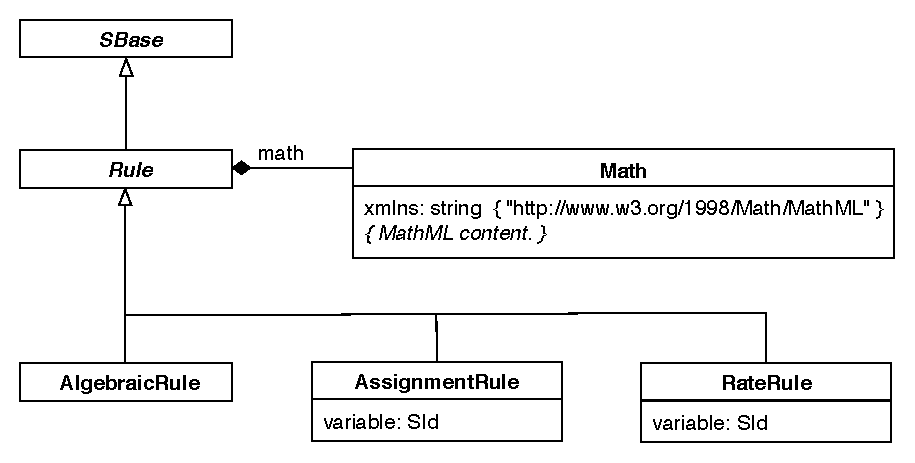
\includegraphics[scale=0.8]{figs/rule-uml}
  \caption{\changed{The definition of \Rule and derived types
      \AlgebraicRule, \AssignmentRule and \RateRule.}}
  \label{fig:rules}
\end{figure}

\clearpage

\subsubsection{Common fields in \abstractclass{Rule}}
\label{sec:rule-math}\label{sec:rule-fields}\label{sec:rule-sboterm}

The subtypes derived from \Rule inherit the \token{math}
and all the \changed{attributes and elements} from \SBase, including \token{sboTerm}.


\paragraph{The \token{math} \changed{element}}

A \Rule \changed{object} has a required \changed{element} called \token{math},
containing a MathML expression defining the mathematical formula
of the rule.  This MathML formula must return a numerical value.
The formula can be an arbitrary expression referencing the
variables and other entities in an SBML model.  The interpretation
of \token{math} and the units of the formula are described in more
detail in Sections~\ref{sec:algebraicrule},
\ref{sec:assignmentrule} and~\ref{sec:raterule} below.


\paragraph{The \token{sboTerm} \changed{attribute}}

The \Rule \changed{object class} inherits from \SBase the optional \token{sboTerm} \changed{attribute} of type
\primtype{SBOTerm} (see Sections~\ref{sec:sboterm-type}
and~\ref{sec:sboTerm}).  When a value is given to this \changed{attribute}, it
must be a valid SBO identifier referring to a mathematical
expression defined in SBO (\ie terms derived from
\sbomathformula).  The \AlgebraicRule, \AssignmentRule, or
\RateRule object should have a ``is a'' relationship with the SBO
term, and the term should be the most precise (narrow) term that
captures the role of that rule in the model.

As discussed in Section~\ref{sec:sboTerm}, SBO labels are optional
information on a model.  Applications are free to ignore
\token{sboTerm} values.  A model must be interpretable without the
benefit of SBO labels.


\subsubsection{\class{AlgebraicRule}}
\label{sec:algebraicrule}

The rule type \AlgebraicRule is used to express equations that are
neither assignments of model variables nor rates of change.
\AlgebraicRule does not add any \changed{attributes} to the basic \Rule; its
role is simply to distinguish this case from the other cases.  An
example of the use of \AlgebraicRule is given in
Section~\ref{sec:algeraiceg}.

In the context of a simulation, algebraic rules are in effect at
all times, $t \geq 0$.  For purposes of evaluating expressions
that involve the \emph{delay} \token{csymbol}
(Section~\ref{sec:csymbol-token}), algebraic rules are considered
to apply also at $t \leq 0$.  Section~\ref{sec:before-t0} provides
additional information about the semantics of assignments, rules,
and entity values for simulation time $t \leq 0$.

The ability to define arbitrary algebraic expressions in an SBML
model introduces the possibility that a model is mathematically
overdetermined by the overall system of equations constructed from
its rules and reactions.  An SBML model must not be
overdetermined; this is discussed in
Section~\ref{sec:ruleconstraints} below.


\subsubsection{\class{AssignmentRule}}
\label{sec:assignmentrule}

The rule type \AssignmentRule is used to express equations that
set the values of variables.  The left-hand side (the
\token{variable} \changed{attribute}) of an assignment rule can refer to the
identifier of a \Species, \Compartment, or \Parameter object in
the model (but not a reaction).  The entity identified must not
have its \token{constant} \changed{attribute} set to \val{true}.  The effects of
an \AssignmentRule are in general terms the same, but differ in
the precise details depending on the type of variable being set:

\begin{itemize}
  
\item \emph{In the case of a species}, an \AssignmentRule sets the
  referenced species' quantity (\quantity{concentration} or
  \quantity{amount of substance}) to the value determined by the
  formula in \token{math}.  The units of the formula in
  \token{math} must be the same as the \emph{units of the species}
  (Section~\ref{sec:species-units}) for the species identified by
  the \token{variable} \changed{attribute} of the \AssignmentRule.
  
  \emph{Restrictions}: There must not be both an \AssignmentRule
  \token{variable} \changed{attribute} and a \SpeciesReference \token{species}
  \changed{attribute} having the same value, unless that species has its
  \token{boundaryCondition} \changed{attribute} set to \val{true}.  In other
  words, an assignment rule cannot be defined for a species that
  is created or destroyed in a reaction unless that species is
  defined as a boundary condition in the model.

\item \emph{In the case of a compartment}, an \AssignmentRule sets
  the referenced compartment's size to the value determined by the
  formula in \token{math}.  The overall units of the formula in
  \token{math} must be the same as the units of the size of the
  compartment (Section~\ref{sec:compartment-units}).
  
\item \emph{In the case of a parameter}, an \AssignmentRule sets
  the referenced parameter's value to that determined by the
  formula in \token{math}.  The overall units of the formula in
  \token{math} must be the same as the units defined for the
  parameter (Section~\ref{sec:parameter-units}).

\end{itemize}

In the context of a simulation, assignment rules are in effect at
all times, $t \geq 0$.  For purposes of evaluating expressions
that involve the \emph{delay} \token{csymbol}
(Section~\ref{sec:csymbol-token}), assignment rules are considered
to apply also at $t \leq 0$.  Section~\ref{sec:before-t0} provides
additional information about the semantics of assignments, rules,
and entity values for simulation time $t \leq 0$.

A model must not contain more than one \AssignmentRule or
\RateRule object having the same value of \token{variable}; in
other words, in the set of all assignment rules and rate rules in
an SBML model, each variable appearing in the left-hand sides can
only appear once.  This simply follows from the fact that an
indeterminate system would result if a model contained more than
one assignment rule for the same variable or both an assignment
rule and a rate rule for the same variable.

Similarly, a model must also not contain \emph{both} an
\AssignmentRule and an \InitialAssignment for the same variable,
because both kinds of constructs apply prior to and at the start
of simulation time, \ie $t \leq 0$.  If a model contained both an
initial assignment and an assignment rule for the same variable,
an indeterminate system would result.  (See also
Section~\ref{sec:initial-assignment-semantics}.)

The value calculated by an \AssignmentRule object overrides the
value assigned to the given symbol by the object defining that
symbol.  For example, if a \Compartment's \token{size} is set in
its definition, and the model also contains an \AssignmentRule
having that compartment's \token{id} as its \token{variable}
value, then the \token{size} assigned in the \Compartment
definition is ignored and the value assigned based on the
computation defined in the \AssignmentRule.  This does \emph{not}
mean that a definition for a given symbol can be omitted if there
is an \AssignmentRule object for it.  For example, there must be a
\Parameter definition for a given parameter if there is an
\AssignmentRule for that parameter.


\subsubsection{\class{RateRule}}
\label{sec:raterule}

The rule type \RateRule is used to express equations that
determine the rates of change of variables.  The left-hand side
(the \token{variable} \changed{attribute}) can refer to the identifier of a
species, compartment, or parameter (but not a reaction).  The
entity identified must have its \token{constant} \changed{attribute} set to
\val{false}.  The effects of a \RateRule are in general terms the
same, but differ in the precise details depending on which
variable is being set:

\begin{itemize}
  
\item \emph{In the case of a species}, a \RateRule sets the rate
  of change of the species' quantity (\quantity{concentration} or
  \quantity{amount of substance}) to the value determined by the
  formula in \token{math}.  The overall units of the formula in
  \token{math} must be \quantity{species
    quantity}/\quantity{time}, where the \quantity{time} units are
  the built-in units of time described in
  Section~\ref{sec:unitdefinitions} and the \quantity{species
    quantity} units are the \emph{units of the species} as defined
  in Section~\ref{sec:species-units}.
  
  \emph{Restrictions}: There must not be both a \RateRule
  \token{variable} \changed{attribute} and a \SpeciesReference \token{species}
  \changed{attribute} having the same value, unless that species has its
  \token{boundaryCondition} \changed{attribute} is set to \val{true}.  This
  means a rate rule cannot be defined for a species that is
  created or destroyed in a reaction, unless that species is
  defined as a boundary condition in the model.
  
\item \emph{In the case of a compartment}, a \RateRule sets the
  rate of change of the compartment's size to the value determined
  by the formula in \token{math}.  The overall units of the
  formula must be \quantity{size}/\quantity{time}, where the
  \quantity{time} units are the built-in units of time described
  in Section~\ref{sec:unitdefinitions} and the \quantity{size}
  units are the units of size on the compartment
  (Section~\ref{sec:compartment-units}).

\item \emph{In the case of a parameter}, a \RateRule sets the rate
  of change of the parameter's value to that determined by the
  formula in \token{math}.  The overall units of the formula must
  be \quantity{x}/\quantity{time}, where \quantity{x} are the
  units of the parameter (Section~\ref{sec:parameter-units}).

\end{itemize}

In the context of a simulation, rate rules are in effect for
simulation time $t > 0$.  Other types of rules and initial
assignments are in effect at different times;
Section~\ref{sec:before-t0} describes these conditions.

As mentioned in Section~\ref{sec:assignmentrule} for
\AssignmentRule, a model must not contain more than one \RateRule
or \AssignmentRule object having the same value of
\token{variable}; in other words, in the set of all assignment
rules and rate rules in an SBML model, each variable appearing in
the left-hand sides can only appear once.  This simply follows
from the fact that an indeterminate system would result if a model
contained more than one assignment rule for the same variable or
both an assignment rule and a rate rule for the same variable.


\subsubsection{Additional restrictions on rules}
\label{sec:ruleconstraints}

An important design goal of SBML rule semantics is to ensure that
a model's simulation and analysis results will not be dependent on
when or how often rules are evaluated.  To achieve this, SBML
needs to place two additional restrictions on rule use in addition
to the conditions described above regarding the use of
\AlgebraicRule, \AssignmentRule and \RateRule.  The first concerns
algebraic loops in the system of assignments in a model, and the
second concerns overdetermined systems.


\paragraph{The model must not contain algebraic loops}

The combined set of \InitialAssignment, \AssignmentRule and
\KineticLaw objects constitute a set of assignment statements that
should be considered as a whole.  (A \KineticLaw object is counted
as an assignment because it assigns a value to the symbol
contained in the \token{id} \changed{attribute} of the \Reaction object in which
it is defined.)  This combined set of assignment statements must
not contain algebraic loops---dependency chains between these
statements must terminate.  To put this more formally, consider a
directed graph in which nodes are assignment statements and
directed arcs exist for each occurrence of an SBML species,
compartment or parameter symbol in an assignment statement's
\token{math} \changed{element}.  Let the directed arcs point from the
statement assigning the symbol to the statements that contain the
symbol in their \token{math} \changed{element} expressions.  This graph must
be acyclic.

SBML does not specify when or how often rules should be evaluated.
Eliminating algebraic loops ensures that assignment statements can
be evaluated any number of times without the result of those
evaluations changing.  As an example, consider the following
equations:
\begin{linenomath}
\begin{equation*}
  \begin{array}{lll}
    x = x + 1, & y = z + 200, & z = y + 100
  \end{array}
\end{equation*}
\end{linenomath}
If this set of equations were interpreted as a set of assignment
statements, it would be invalid because the rule for $x$ refers to
$x$ (exhibiting one type of loop), and the rule for $y$ refers to
$z$ while the rule for $z$ refers back to $y$ (exhibiting another
type of loop).

Conversely, the following set of equations would constitute a
valid set of assignment statements:
\begin{linenomath}
\begin{equation*}
  \begin{array}{lll}
    x = 10, & y = z + 200, & z = x + 100
  \end{array}
\end{equation*}
\end{linenomath}


\paragraph{The model must not be overdetermined}

An SBML model must not be overdetermined; that is, a model must
not define more equations than there are unknowns in a model.  An
SBML model that does not contain \AlgebraicRule \changed{objects} cannot
be overdetermined.

Assessing whether a given continuous, deterministic, mathematical
model is overdetermined does not require dynamic analysis; it can
be done by analyzing the system of equations created from the
model.  One approach is to construct a bipartite graph in which
one set of vertices represents the variables and the other the set
of vertices represents the equations.  Place edges between
vertices such that variables in the system are linked to the
equations that determine them.  For algebraic equations, there
will be edges between the equation and each variable occurring in
the equation.  For ordinary differential equations (such as those
defined by rate rules or implied by the reaction rate
definitions), there will be a single edge between the equation and
the variable determined by that differential equation.  A
mathematical model is overdetermined if the maximal
matchings~\citep{chartrand_1977} of the bipartite graph contain
disconnected vertexes representing equations.  (If one maximal
matching has this property, then all the maximal matchings will
have this property; \ie it is only necessary to find one maximal
matching.)  Appendix~\ref{apdx:assessing-overdetermined} describes
a method of applying this procedure to specific SBML data objects.


\subsubsection{Example of rule use}
\label{sec:eg-rule-use}

This section contains an example set of rules.  Consider the
following set of equations:
\begin{linenomath}
  \begin{equation*}
    \begin{array}{lll}
      k = \dfrac{k_3}{k_2}, & s_2 = \dfrac{k \cdot x}{1 + k_2}, & A = 0.10 \cdot x
    \end{array}
  \end{equation*}
\end{linenomath}
This can be encoded by the following scalar rule set (where the
definitions of \texttt{x}, \texttt{s}, \texttt{k}, \texttt{k2},
\texttt{k3} and \texttt{A} are assumed to be located elsewhere in
the model and not shown in this abbreviated example):

\begin{example}
    <listOfRules>
        <assignmentRule variable="k">
            <math xmlns="http://www.w3.org/1998/Math/MathML">
                <apply>
                    <divide/>
                    <ci> k3 </ci>
                    <ci> k2 </ci>
                </apply>
            </math>
        </assignmentRule>
        <assignmentRule variable="s2">
            <math xmlns="http://www.w3.org/1998/Math/MathML">
                <apply>
                    <divide/>
                    <apply>
                        <times/>
                        <ci> k </ci>
                        <ci> x </ci>
                    </apply>
                    <apply>
                        <plus/>
                        <cn> 1 </cn>
                        <ci> k2 </ci>
                    </apply>
                </apply>
            </math>
        </assignmentRule>
        <assignmentRule variable="A">
            <math xmlns="http://www.w3.org/1998/Math/MathML">
                <apply>
                    <times/>
                    <cn> 0.10 </cn>
                    <ci> x </ci>
                </apply>
            </math>
        </assignmentRule>
    </listOfRules>
\end{example}


%\subsubsection{Guidelines for Evaluating Rules}
%
%This section describes how rules including those implied by
%\Reaction structures (see Section~\ref{sec:reactions})
%should be evaluated.  For the purpose of interpreting models
%mathematically (and for this description), \Reaction
%structures collectively imply a \class{SpeciesConcentrationRule}
%structure, of type \class{rate}, for each species referenced in a
%\SpeciesReference structure excluding those species which
%are defined with the \token{boundaryCondition} attribute equal to
%\texttt{true}.
%
%To determine the initial values of variables is a 2 set process:
%
%\begin{itemize}
%
%\item variables should be set according to the initial values
%given by \Species, \Compartment and
%\Parameter structures then
%
%\item the \class{scalar} rules should be evaluated
%
%\end{itemize}
%
%To determine the rates of change of variables given a set of
%current variable values is again a two set process:
%
%\begin{itemize}
%
%\item the \class{scalar} rules should be evaluated then
%
%\item the \class{rate} rules should be evaluated
%
%\end{itemize}
%
%The \class{scalar} rules should be evaluated to determine the
%complete set of variable values given an incomplete set of
%variable values determined by \class{rate} and
%\AlgebraicRule structures.
%


%-----------------------------------------------------------------------------
\subsection{Constraints}
\label{sec:constraints}
%-----------------------------------------------------------------------------

The \Constraint object is a mechanism for stating the
assumptions under which a model is designed to operate.  The
\emph{constraints} are statements about permissible values of
different quantities in a model.  Figure~\vref{fig:constraint}
shows the definition of the \Constraint \changed{object class}.

\begin{figure}[htb]
  \centering
  \small
  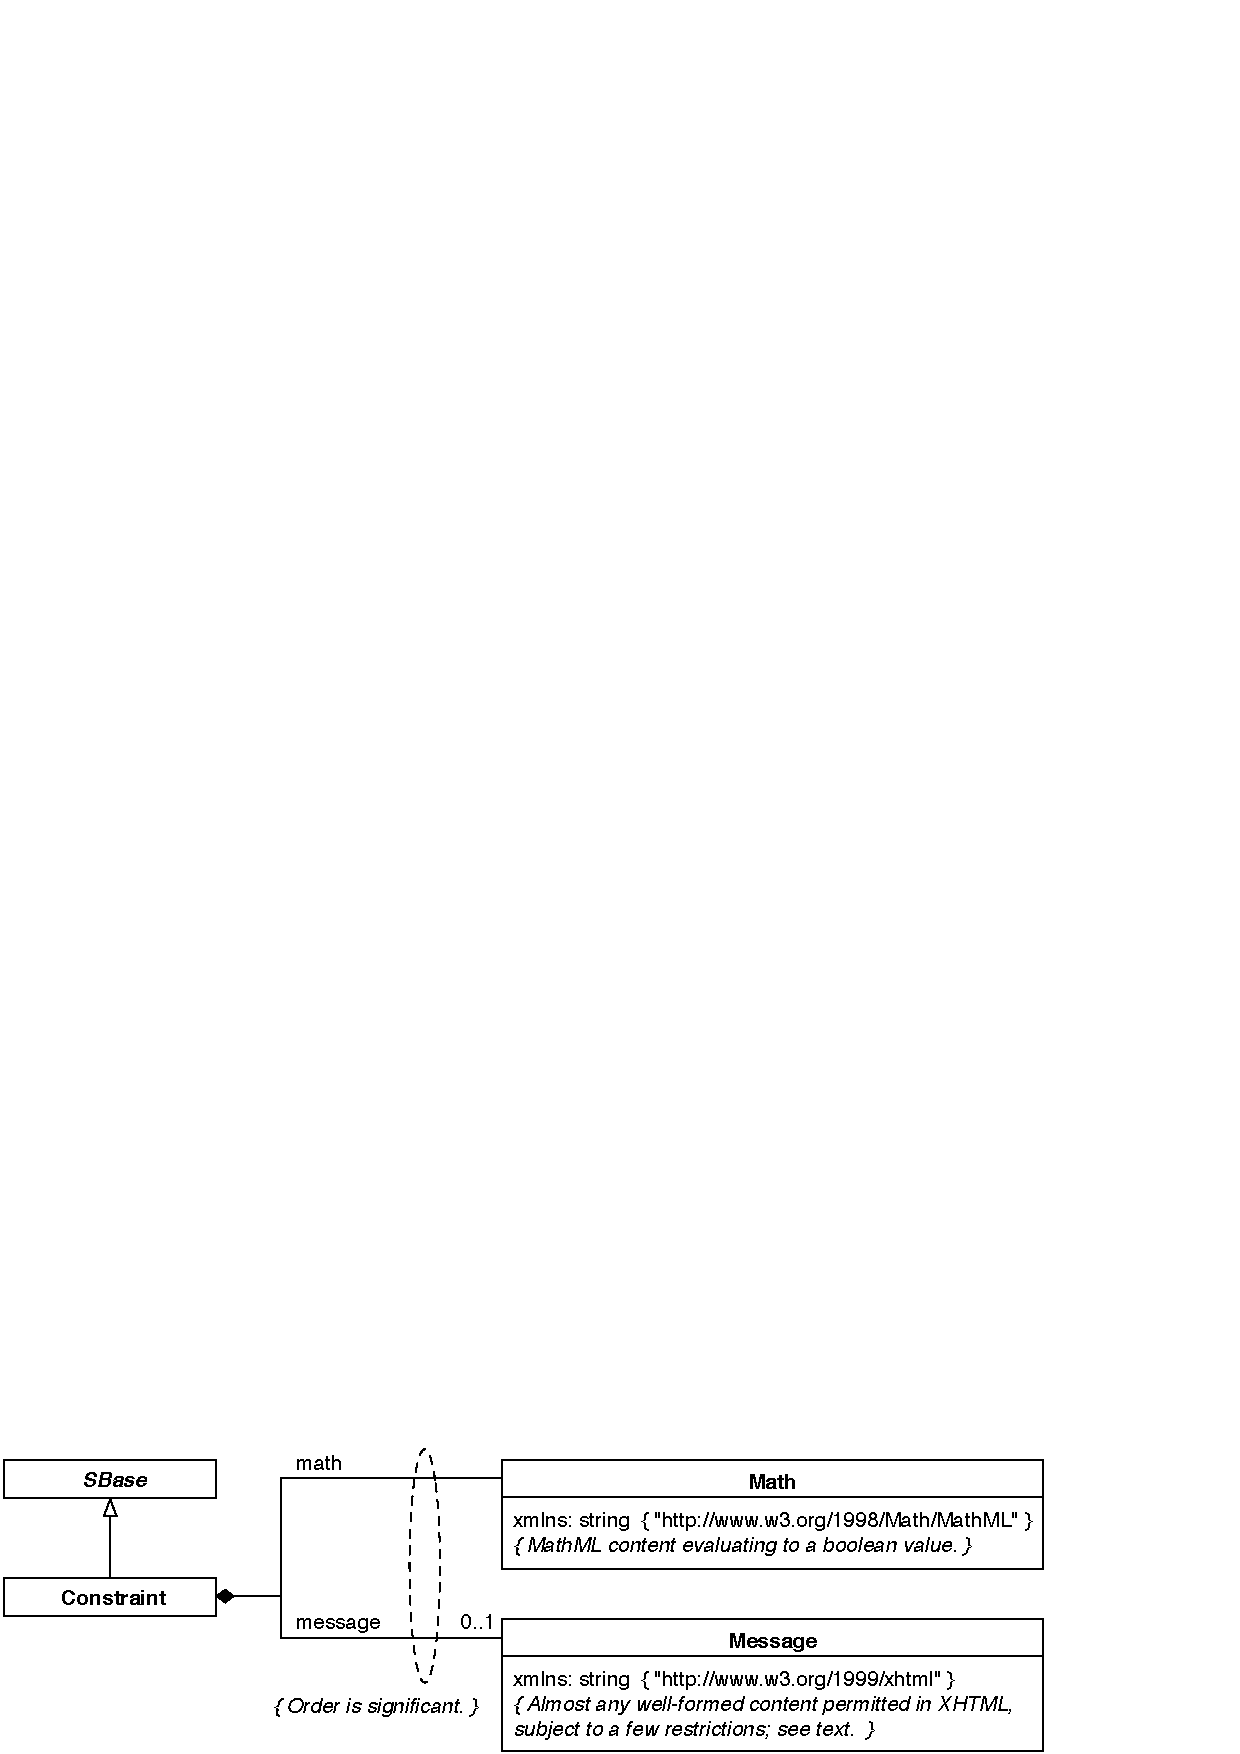
\includegraphics[scale=0.8]{figs/constraint-uml}
  \caption{\changed{The definition of class \Constraint.  The
      contents of the \class{Math} class can be any \mathml
      permitted in SBML, but it must return a boolean value.  As
      shown above, an instance of \Constraint can also contain
      zero or one instances of \class{Message}; this element is
      simply a wrapper (in the XML form, within \token{<message>
        \ldots{} </message>} tags) for XHTML content.  The same
      guidelines for XHTML content as explained in
      Section~\ref{sec:notes} for notes on \SBase also apply to
      the XHTML within messages in a \Constraint. A sequence of
      one or more instances of \Constraint objects can be located
      in an instance of \ListOfConstraints in \Model, as shown in
      Figure~\protect\ref{fig:model}.}}
  \label{fig:constraint}
\end{figure}


\subsubsection{The \token{math} \changed{element}}

\Constraint has one required \changed{subelement}, \token{math},
containing a MathML formula defining the condition of the
constraint.  This formula must return a boolean value of
\val{true} when the model is in a \emph{valid} state.  The formula
can be an arbitrary expression referencing the variables and other
entities in an SBML model.  The evaluation of \token{math} and
behavior of constraints are described in more detail in
Section~\ref{sec:constraint-semantics} below.


\subsubsection{The \token{message} \changed{element}}
\label{sec:constraint-message}

A \Constraint \changed{object} has an optional \changed{element} called
\token{message}.  This can contain a message in XHTML format that
may be displayed to the user when the condition of the constraint
in \token{math} evaluates to a value of \val{false}.  Software
tools are not required to display the message, but it is
recommended that they do so as a matter of best practice.

\begin{blockChanged}

The XHTML content within a \token{message} element must follow the
same restrictions as for the \token{notes} element on \SBase
described in Section~\ref{sec:notes}.  For example,
\token{message} must not contain an XML declaration or a DOCTYPE
declaration, and the permitted content can only take one of the
following general forms: (1) a complete XHTML document beginning
with the element \token{<html>} and ending with \token{</html>};
(2) the ``body'' portion of a document beginning with the element
\token{<body>} and ending with \token{</body>}; or (3) XHTML
content that is permitted within a \token{<body>} ...
\token{</body>} elements.    Appendix~\ref{apdx:processing-notes}
describes one approach to reading the \token{message} content.

\end{blockChanged}


\subsubsection{The \token{sboTerm} \changed{attribute}}
\label{sec:constraint-sboterm}

The \Constraint \changed{object} inherits from \SBase the optional \token{sboTerm} \changed{attribute} of
type \primtype{SBOTerm} (see Sections~\ref{sec:sboterm-type}
and~\ref{sec:sboTerm}).  When a value is given to this \changed{attribute} in a
constraint definition, the value must be a valid SBO identifier
referring to a mathematical expression (\ie terms derived from
\sbomathformula).  The \Constraint should have an ``is a''
relationship with the SBO term, and the term should be the most
precise (narrow) term that captures the role of the \Constraint in
the model.

As discussed in Section~\ref{sec:sboTerm}, SBO labels are optional
information on a model.  Applications are free to ignore
\token{sboTerm} values.  A model must be interpretable without the
benefit of SBO labels.


\subsubsection{Semantics of constraints}
\label{sec:constraint-semantics}

In the context of a simulation, a \Constraint has effect at all
times $t \geq 0$.  Each \Constraint's \token{math} \changed{element} is first
evaluated after any \InitialAssignment definitions in a model at
$t = 0$ and can conceivably trigger at that point.  (In other
words, a simulation could fail a constraint immediately.)

\Constraint \changed{definitions} \emph{cannot and should not} be used to
compute the dynamical behavior of a model as part of, for example,
simulation.  Constraints may be used as input to non-dynamical
analysis, for instance by expressing flux constraints for flux
balance analysis.

The results of a simulation of a model containing a constraint are
invalid from any simulation time at and after a point when the
function given by the \token{math} returns a value of \val{false}.
Invalid simulation results do not make a prediction of the
behavior of the biochemical reaction network represented by the
model.  The precise behavior of simulation tools is left undefined
with respect to constraints.  If invalid results are detected with
respect to a given constraint, the \token{message} \changed{element}
(Section~\ref{sec:constraint-message}) may optionally be displayed
to the user.  The simulation tool may also halt the simulation or
clearly delimit in output data the simulation time point at which
the simulation results become invalid.

SBML does not impose restrictions on duplicate \Constraint
definitions or the order of evaluation of \Constraint objects in a
model.  It is possible for a model to define multiple constraints
all with the same \token{math} \changed{element}.  Since the failure of any
constraint indicates that the model simulation has entered an
invalid state, a system is not required to attempt to detect
whether other constraints in the model have failed once any one
constraint has failed.


\subsubsection{Example}

As an example, the following SBML fragment demonstrates the
constraint that species $S_1$ should only have values between 1
and 100:

\begin{blockChanged}

\begin{example}
<model>
    ...
    <listOfConstraints>
        <constraint>
            <math xmlns="http://www.w3.org/1998/Math/MathML">
                <apply>
                    <and/>
                    <apply>
                        <lt/>
                        <cn> 1 </cn>
                        <ci> S1 </ci>
                    </apply>
                    <apply>
                        <lt/>
                        <ci> S1 </ci>
                        <cn> 100 </cn>
                    </apply>
                </apply>
            </math>
            <message>
                <p xmlns="http://www.w3.org/1999/xhtml"> Species S1 is out of range. </p>
            </message>
        </constraint>
    </listOfConstraints>
    ...
</model>
\end{example}
\end{blockChanged}


%-----------------------------------------------------------------------------
\subsection{Reactions}
\label{sec:reactions}
%-----------------------------------------------------------------------------

A \emph{reaction} represents any transformation, transport or
binding process, typically a chemical reaction, that can change
the quantity of one or more species.  In SBML, a reaction is
defined primarily in terms of the participating reactants and
products (and their corresponding stoichiometries), along with
optional modifier species, an optional rate at which the reaction
takes place, and optional parameters.  These various parts of a
reaction are recorded in the SBML \Reaction \changed{object class} and other
supporting data \changed{classes}, defined in Figure~\vref{fig:reaction}.

\begin{figure}[htb]
  \centering
  \vspace*{1ex}
  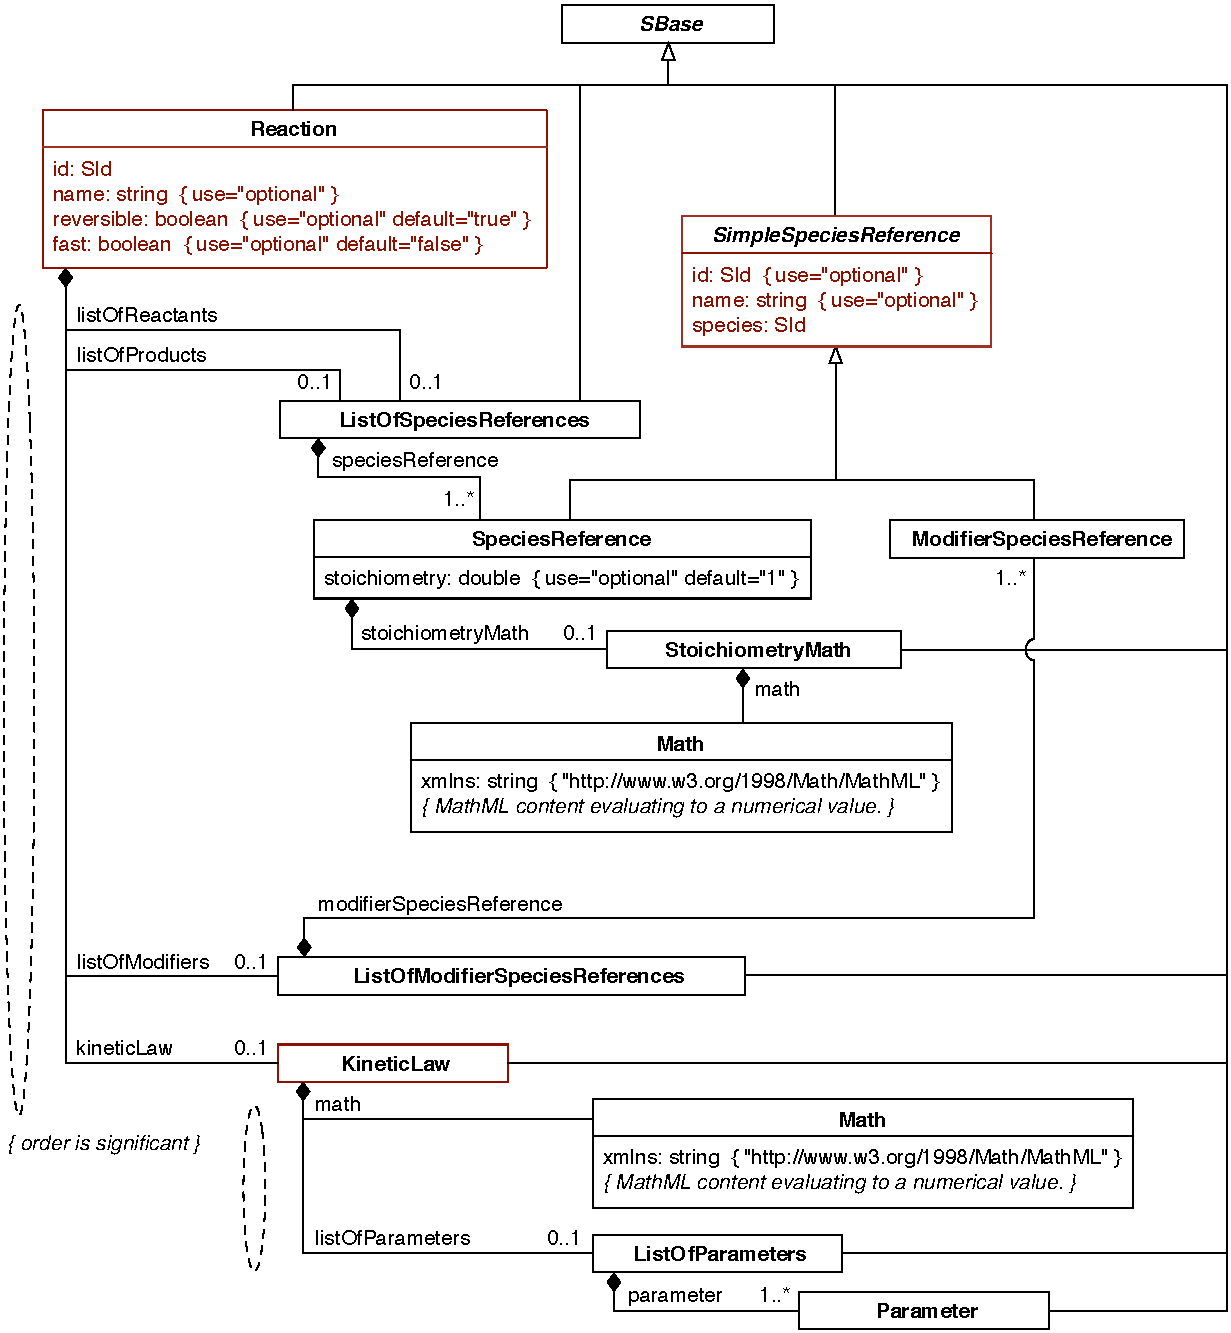
\includegraphics[scale=0.779]{figs/reaction-uml-v2}
  \vspace*{0.5ex}
  \caption{\changed{The definitions of classes \Reaction, \KineticLaw,
      \SpeciesReference, \ModifierSpeciesReference, as well as the
      container classes \ListOfReactants, \ListOfProducts,
      \ListOfModifiers, and \ListOfParameters.  Note that
      \SimpleSpeciesReference is an abstract class used only to
      provide some common attributes to its derived classes.  The class
      \Parameter is defined in Section~\ref{sec:parameters}.}}
  \label{fig:reaction}
\end{figure}


% fixme: need to write that if stoichiometryMath is present,
% the attribute stoichiometry is ignored.


\subsubsection{class{Reaction}}
\label{sec:reaction-type}
\label{sec:listofreactants}
\label{sec:listofproducts}
\label{sec:listofmodifiers}

Each reaction in an SBML model is defined using an instance of a
\Reaction \changed{object}.  As shown in Figure~\vref{fig:reaction}, it
contains several scalar \changed{attributes} and several lists of objects.


\paragraph{The \token{id} and \token{name} \changed{attributes}}

As with most other main \changed{kinds of objects} in SBML, the
\Reaction \changed{object class}
includes a mandatory \changed{attribute} called \token{id}, of type
\primtype{SId}, and an optional \changed{attribute} \token{name}, of type
\primtype{string}.  The \token{id} \changed{attribute} is used to give the
reaction a unique identifier in the model.  This identifier can be
used in mathematical formulas elsewhere in an SBML model to
represent the rate of that reaction; this usage is explained in
detail in Section~\ref{subsec:reaction-as-symbol} below.  The
\token{name} \changed{attribute} can be used to give the reaction a more
free-form, descriptive name.  The \token{name} and \token{id}
\changed{attributes} must be used as described in
Section~\ref{sec:idnameattribs}.


\paragraph{The lists of reactants, products and modifiers}

The species participating as reactants, products, and/or modifiers
in a reaction are declared using lists of \SpeciesReference and/or
\ModifierSpeciesReference instances stored in
\token{listOfReactants}, \token{listOfProducts} and
\token{listOfModifiers}.  \changed{\SpeciesReference and
\ModifierSpeciesReference} are described in more detail
in Sections~\ref{subsec:speciesreference}
and~\ref{subsec:modifierreference} below.

Certain restrictions are placed on the appearance of species in
reaction definitions:
\begin{itemize}
  
\item The ability of a species to appear as a reactant or product
  of any reaction in a model is governed by certain flags in that
  species' definition; see Section~\ref{sec:species-constant} for
  more information.
  
\item Any species appearing in the mathematical formula of the
  \token{kineticLaw} of a \Reaction instance must be declared in
  at least one of that \Reaction's lists of reactants, products,
  and/or modifiers.  Put another way, it is an error for a
  reaction's kinetic law formula to refer to species that have not
  been declared for that reaction.
  
\item A reaction definition can contain an empty list of reactants
  \emph{or} an empty list of products, but it must have at least
  one reactant or product; in other words, a reaction without any
  reactant or product species is not permitted.  (This restriction
  does not apply to modifier species, which remain optional in all
  cases.)

\end{itemize}


\paragraph{The \token{kineticLaw} \changed{element}}

A reaction can contain up to one \KineticLaw \changed{object} in the
\token{kineticLaw} \changed{element} of the \Reaction.  This ``kinetic law''
defines the speed at which the process defined by the reaction
takes place.  A detailed description of \KineticLaw is left to
Section~\ref{subsec:kinetic-law} below.

Note that the inclusion of a \KineticLaw \changed{object} in an instance
of a \Reaction component is optional; however, in general there is
no useful default that can be substituted in place of a missing
rate expression in a reaction.  Moreover, a reaction's rate cannot
be defined in any other way in SBML---\InitialAssignment,
\AssignmentRule, \RateRule, \AlgebraicRule, \Event, and other
constructs in SBML cannot be used to set the reaction rate
separately.  Nevertheless, for some modeling applications,
reactions without any defined rate can be perfectly acceptable.


\paragraph{The \token{reversible} \changed{attribute}}
\label{sec:reversible}

The optional boolean \changed{attribute} \token{reversible} indicates whether
the reaction is reversible.  The default is \val{true}.

To say that a reaction is \emph{reversible} is to say it can
proceed in either the forward or the reverse direction.  Although
the reversibility of a reaction can sometimes be deduced by
inspecting its rate expression, this is not always the case,
especially for complicated expressions.  Having a separate \changed{attribute}
supports the ability to perform some kinds of model analyses in
the absence of performing a time-course simulation of the model.
Moreover, the need in SBML to allow rate expressions (\ie
\KineticLaw) to be optional leads to the need for a separate flag
indicating reversibility.  Information about reversibility in the
absence of a \KineticLaw in a \Reaction is useful in certain kinds
of structural analyses such as elementary mode analysis.

Mathematically, the \token{reversible} \changed{attribute} on \Reaction has no
impact on the construction of the equations giving the overall
rates of change of each species quantity in a model.  A concrete
explanation may help illustrate this.  Suppose a model consists of
multiple reactions, of which two particular irreversible reactions
$R_f$ and $R_r$ are actually the forward and reverse processes of
the same underlying reaction.  The product species of $R_f$
necessarily will be the reactants of $R_r$, and the reactants of
$R_f$ will be the products of $R_r$.  Let $f_f(\mathbf{X})$ and
$f_r(\mathbf{X})$ be the SBML kinetic rate formulas of $R_f$ and
$R_r$, respectively, with $\mathbf{X}$ representing the species,
parameters and compartments in the model.  For the sake of this
example, suppose we are using a continuous differential equation
framework to simulate the system of reactions.  Then for each
species, we need to construct an expression representing the
overall rate of change of that species' amount in the model.  This
overall expression will be a sum of the contributions of all the
relevant rate formulas,
\begin{linenomath}
  \begin{equation*}
    \frac{dS}{dt} =  \ldots - n \! \cdot \! f_f(\mathbf{X}) + n \! \cdot \! f_r(\mathbf{X}) + \ldots 
  \end{equation*}
\end{linenomath}
where $S$ is a reactant species of $R_f$ and a product of $R_r$,
$n$ is the effective stoichiometry of $S$ in $R_f$ (which by
implication must be the same as its stoichiometry in $R_r$), and
``\ldots'' indicates other rate formulas in the model involving
the particular species $S$.  Now, contrast this to the case of an
identical second SBML model, except that instead of having
separate \Reaction definitions for the forward and reverse
reactions, this model has a single \Reaction $R_c$ labeled as
reversible and whose reactants and products are the same as those
of $R_f$ in the first model.  The rate of this reaction will be a
formula $f_c$ = $f_f(\mathbf{X}) - f_r(\mathbf{X})$.  In
constructing an expression representing the overall rate of change
for the species $S$ involved in that reaction, we will have
\begin{linenomath}
  \begin{equation*}
    \begin{aligned}
      \dfrac{dS}{dt} & = \ldots - n \! \cdot \! f_c(\mathbf{X}) + \ldots \\
                     & = \ldots - n \! \cdot \! f_f(\mathbf{X}) + n \! \cdot \! f_r(\mathbf{X}) + \ldots 
    \end{aligned}
  \end{equation*}
\end{linenomath}

In other words, the result is the same final expression for the
rate of change of a species.  Although in this simple example we
used an expression for $f_c$ that had clearly separated terms, in
the general case the expression may have a more complicated form.

Note that labeling a reaction as irreversible is an assertion that
the reaction always proceeds in the given forward direction.  (Why
else would it be flagged as irreversible?)  This implies the rate
expression in the \KineticLaw always has a non-negative value
during simulations.  Software tools could provide a means of
optionally testing that this condition holds.  The presence of
reversibility information in two places (\ie the rate expression
and the \token{reversible} flag) leaves open the possibility that
a model could contain contradictory information, but the creation
of such a model would be an error on the part of the software
generating it.


\paragraph{The \token{fast} \changed{attribute}}
\label{sec:fast}

The optional boolean \changed{attribute} \token{fast} is another optional
boolean \changed{attribute} of \Reaction.  The \changed{attribute}'s
default value is \val{false}.

Previous definitions of SBML indicated that software tools could
ignore this \changed{attribute} if they did not implement support for the
corresponding concept; however, further research has revealed that
this is incorrect and \token{fast} \emph{cannot be ignored} if it
is set to \val{true}.  \changed{\sbmltwothree} therefore stipulates that if a
model has any reactions with \token{fast} set to \val{true}, a
software tool must be able to respect the \changed{attribute} or else indicate
to the user that it does not have the capacity to do so.  Analysis
software cannot ignore the value of the \token{fast} attribute
because doing so may lead to different results as compared to a
software system that \emph{does} make use of \token{fast}.

When a model contains true values for \token{fast} on any of its
reactions, it is an indication that the creator of the model is
distinguishing different time scales of reactions in the system.
The model's reaction definitions are divided into two sets by the
values of the \token{fast} \changed{attributes}.  The set of reactions having
\token{fast}=\val{true} (known as \emph{fast reactions}) should be
assumed to be operating on a time scale significantly faster than
the other reactions (the \emph{slow reactions}).  Fast reactions
are considered to be instantaneous relative to the slow reactions.

Software tools must use a pseudo steady-state approximation for
the set of fast reactions when constructing the system of
equations for the model.  More specifically, the set of reactions
that have the \token{fast} attribute set to \val{true} forms a
subsystem that should be described by a pseudo steady-state
approximation in relationship to all other reactions in the model.
Under this description, relaxation from any initial condition or
perturbation from any intermediate state of this subsystem would
be infinitely fast.
Appendix~\ref{apdx:consequences-of-being-fast} provides a
technical explanation of an approach to solving systems with fast
reactions.

The correctness of the approximation requires a significant
separation of time scales between the fast reactions and other
processes.  This is not trivial to estimate a priori, and may even
change over the course of a simulation, but can reasonably be
assessed a posteriori in most cases.


\paragraph{The \token{sboTerm} \changed{attribute} on \class{Reaction}}
\label{sec:reaction-sboterm}

\begin{blockChanged}

The \Reaction \changed{object class} inherits from \SBase the optional
\token{sboTerm} \changed{attribute} of type \primtype{SBOTerm}
(see Sections~\ref{sec:sboterm-type} and~\ref{sec:sboTerm}).  When
a value is given to this \changed{attribute} in a reaction
definition, the value must be a valid SBO identifier referring to
an event (\ie terms derived from \sboevent).  The \Reaction
\changed{object} should have an ``is a'' relationship with the SBO term.
The SBO term chosen should be the most precise (narrow) term that
defines the event represented by the reaction as a whole.  For
example, a given reaction in a model \changed{might represent}
\emph{binding}, which has a term in SBO (identifier
\token{SBO:0000177}, definition ``Interaction between several
biochemical entities that results in the formation of a
non-covalent complex '').  The corresponding \Reaction instance in
SBML would have \token{sboTerm="SBO:0000177"}.

\end{blockChanged}

\changed{As mentioned elsewhere,} SBO labels are optional
information on a model.  Applications are free to ignore
\token{sboTerm} values, and a model must be interpretable without
the benefit of SBO labels.  Section~\ref{sec:sboTerm} gives more
information about this principle and the use of SBO.


\subsubsection{The \class{SimpleSpeciesReference} abstract type}
\label{subsec:simplespeciesreference}

As mentioned above, every species that enters into a given
reaction must appear in that reaction's lists of reactants,
products and/or modifiers.  In an SBML model, all species that may
participate in any reaction are listed in the
\token{listOfSpecies} \changed{element} of the top-level \Model \changed{instance}
(see Section~\ref{sec:model}).  Lists of products, reactants and
modifiers in \Reaction \changed{objects} do not introduce new species,
but rather, they refer back to those listed in the model's
top-level \token{listOfSpecies}.  For reactants and products, the
connection is made using a \SpeciesReference \changed{object}; for
modifiers, it is made using a \ModifierSpeciesReference 
\changed{object}.  \SimpleSpeciesReference, defined in
Figure~\vref{fig:reaction}, is an abstract type that serves as the
parent class of both \SpeciesReference and
\ModifierSpeciesReference.  \changed{It is used simply to hold the attributes
and elements that are common to the latter two objects.}


\paragraph{The \token{id} and \token{name} \changed{attributes}}

The optional identifier stored in the \token{id} \changed{attribute} allows
\SpeciesReference and \ModifierSpeciesReference instances to be
referenced from other \changed{object}.  No SBML \changed{object classes} currently do
this; however, such \changed{classes} are anticipated in future SBML
Levels.  The value of \token{id} must be a text string conforming
to the syntax permitted by the \primtype{SId} data type described
in Section~\ref{sec:sid}.  The \token{id} value (whether it is in
a \SpeciesReference or \ModifierSpeciesReference object) exists in
the global namespace of the model, as described in
Section~\ref{sec:idnameattribs}.  The \token{id} and \token{name}
\changed{attributes} must be used as described in
Section~\ref{sec:idnameattribs}.


\paragraph{The \token{species} \changed{attribute}}

The \SimpleSpeciesReference \changed{object class} has a mandatory \changed{attribute},
\token{species}, of type \primtype{SId}.  As with the other
\changed{attributes}, this \changed{attribute} is inherited by the \SpeciesReference and
\ModifierSpeciesReference subtypes derived from
\SimpleSpeciesReference.  The value of \token{species} must be the
identifier of a species defined in the enclosing \Model.  The
species is thereby declared as participating in the reaction being
defined.  The precise role of that species as a reactant, product,
or modifier in the reaction is determined by the subtype of
\SimpleSpeciesReference (\ie either \SpeciesReference or
\ModifierSpeciesReference) in which the identifier appears.


\paragraph{The \token{sboTerm} \changed{attribute}}
\label{sec:simplespeciesreference-sboterm}

\changed{The class} \SimpleSpeciesReference inherits from \SBase
the optional \token{sboTerm} \changed{attribute} of type
\primtype{SBOTerm} (see Sections~\ref{sec:sboterm-type}
and~\ref{sec:sboTerm}).  This means that the object classes
derived from \SimpleSpeciesReference, namely \SpeciesReference and
\ModifierSpeciesReference, all have \token{sboTerm}
\changed{attributes}.  When a value is given to this
\changed{attribute}, it must be a valid SBO \changed{identifier}
referring to a participant role.  The appropriate \changed{SBO}
term depends on whether the object is a reactant, product or
modifier.  If a reactant, then it should be a term in the
\sboreactant hierarchy; if a product, then it should be a term in
the \sboproduct hierarchy; and if a modifier, then it should be a
term in the \sbomodifier hierarchy.  The \SpeciesReference and
\ModifierSpeciesReference instances should have an ``is a''
relationship to the term identified by the SBO identifier.

\begin{blockChanged}

The SBO terms chosen should be the most precise (narrow) one that
defines the role of the species in the reaction.  As might be
expected, an SBO reactant term can only be assigned to the
\token{sboTerm} attribute of a \SpeciesReference instance when
that instance is contained in the list of reactants in the
containing \Reaction instance.  Similarly, an SBO product term can
only be assigned to the \token{sboTerm} attribute of a
\SpeciesReference instance when that instance is contained in the
list of products in the containing \Reaction instance.

\end{blockChanged}


\subsubsection{\class{SpeciesReference}}
\label{subsec:speciesreference}

The \Reaction \changed{object class} provides a way to express which species
act as reactants and which species act as products in a reaction.
In a given reaction, references to those species acting as
reactants and/or products are made using instances of
\SpeciesReference \changed{objects} in \Reaction's lists of reactants and
products.  The \SpeciesReference structure inherits the mandatory
\changed{attribute} \token{species} and optional \changed{attributes} \token{id},
\token{name}, and \token{sboTerm}, from the parent type
\SimpleSpeciesReference; see
Section~\ref{subsec:simplespeciesreference} for their definitions.
It also defines \changed{attribute} \token{stoichiometry} and
\changed{element} \token{stoichiometryMath}, described below.

The \token{species} \changed{attribute} value must be the
identifier of an existing species defined in the enclosing \Model;
the species is thereby designated as a reactant or product in the
reaction.  Which one it is (\ie reactant or product) is indicated
by whether the \SpeciesReference appears in the \Reaction's
\token{reactant} or \token{product} lists.


\paragraph{The \token{stoichiometry} \changed{attribute} and \token{stoichiometryMath}
  \changed{element}}

Product and reactant stoichiometries can be specified using
\emph{either} \token{stoichiometry} or \token{stoichiometryMath}
in a \SpeciesReference \changed{object}.  The \token{stoichiometry}
\changed{attribute} is of type double and should contain values greater than
zero (0).  The \token{stoichiometryMath} \changed{element} is implemented as
an element containing a MathML expression.  These two are
mutually exclusive; only one of \token{stoichiometry} or
\token{stoichiometryMath} should be defined in a given
\SpeciesReference instance.  When neither \changed{the attribute
  nor the element} is present, the
value of \token{stoichiometry} in the \SpeciesReference instance
defaults to \val{1}.

For maximum interoperability, the \token{stoichiometry} \changed{attribute}
should be used in preference to \token{stoichiometryMath} when a
species' stoichiometry is a simple scalar number (integer or
decimal).  When the stoichiometry is a rational number, or when it
is a more complicated formula, \token{stoichiometryMath} must be
used.  The MathML expression in \token{stoichiometryMath} may also
refer to identifiers of entities in a model (except reaction
identifiers), as discussed in Section~\ref{sec:ci-token}.
However, the only species identifiers that can be used in
\token{stoichiometryMath} are those referenced in the \Reaction
list of reactants, products and modifiers.

The following is a simple example of a species reference for
species \val{X0}, with stoichiometry \val{2}, in a list of
reactants within a reaction having the identifier \val{J1}:

\begin{example}
<model>
    ...
    <listOfReactions>
        <reaction id="J1">
            <listOfReactants>
                <speciesReference species="X0" stoichiometry="2">
            </listOfReactants>
            ...
        </reaction>
        ...
    </listOfReactions>
    ...
</model>
\end{example}

The following is a more complex example of a species reference for
species ``X0'', with a stoichiometry formula consisting of the
parameter \texttt{x}:

\begin{example}
<model>
    ...
    <listOfReactions>
        <reaction id="J1">
            <listOfReactants>
                <speciesReference species="X0">
                    <stoichiometryMath>
                        <math xmlns="http://www.w3.org/1998/Math/MathML">
                            <ci>x</ci>
                        </math>
                    </stoichiometryMath>
                </speciesReference>
            </listOfReactants>
            ...
        </reaction>
        ...
    </listOfReactions>
    ...
</model>
\end{example}

A species can occur more than once in the lists of reactants and
products of a given \Reaction instance.  The effective
stoichiometry for a species in a reaction is the sum of the
stoichiometry values given in the \SpeciesReference \changed{objects} in
the list of products minus the sum of stoichiometry values given
in the \SpeciesReference \changed{objects} in the list of reactants.  A
positive value indicates the species is effectively a product and
a negative value indicates the species is effectively a reactant.
SBML places no restrictions on the effective stoichiometry of a
species in a reaction; for example, it can be zero.  In the
following SBML fragment, the two reactions have the same effective
stoichiometry for all their species:

\begin{example}
<reaction id="x">
    <listOfReactants>
        <speciesReference species="a"/>
        <speciesReference species="a"/>
        <speciesReference species="b"/>
    </listOfReactants>
    <listOfProducts>
        <speciesReference species="c"/>
        <speciesReference species="b"/>
    </listProducts>
</reaction>
<reaction id="y">
    <listOfReactants>
        <speciesReference species="a" stoichiometry="2"/>
    </listOfReactants>
    <listOfProducts>
        <speciesReference species="c"/>
    </listProducts>
</reaction>
\end{example}


\subsubsection{\class{ModifierSpeciesReference}}
\label{subsec:modifierreference}

Sometimes a species appears in the kinetic rate formula of a
reaction but is itself neither created nor destroyed in that
reaction (for example, because it acts as a catalyst or
inhibitor).  In SBML, all such species are simply called
\emph{modifiers} without regard to the detailed role of those
species in the model.  The \Reaction \changed{object class} provides a way to
express which species act as modifiers in a given reaction.  This
is the purpose of the list of modifiers available in \Reaction.
The list contains instances of \ModifierSpeciesReference
\changed{object}.

As shown in Figure~\vref{fig:reaction}, the
\ModifierSpeciesReference \changed{class} inherits the mandatory \changed{attribute}
\token{species} and optional \changed{attributes} \token{id} and \token{name}
from the parent class \SimpleSpeciesReference; see
Section~\ref{subsec:simplespeciesreference} for their precise
definitions.

The value of the \token{species} \changed{attribute} must be the identifier of a
species defined in the enclosing \Model; this species is
designated as a modifier for the current reaction.  A reaction may
have any number of modifiers.  It is permissible for a modifier
species to appear simultaneously in the list of reactants and
products of the same reaction where it is designated as a
modifier, as well as to appear in the list of reactants, products
and modifiers of other reactions in the model.


\subsubsection{\class{KineticLaw}}
\label{subsec:kinetic-law}

The \KineticLaw \changed{object class} is used to describe the rate at which
the process defined by the \Reaction takes place.  As shown in
Figure~\vref{fig:reaction}, \KineticLaw has \changed{elements} called
\token{math} and \changed{\token{listOfParameters}}, in addition to the
\changed{attributes and elements} it inherits from \SBase.

Previous definitions of SBML included two additional \changed{attributes} called
\token{substanceUnits} and \token{timeUnits}, which allowed the
\quantity{substance}/\quantity{time} units of the reaction rate
expression to be defined on a per-reaction basis.  \changed{\sbmltwotwo
and Version~3 removed} these \changed{attributes} for several reasons.  First, the introduction
in \sbmltwotwo of mass and dimensionless units as possible units
of \quantity{substance}, coupled with the previous facility for
defining the units of each reaction separately and the ability to
use non-integer stoichiometries, lead to the possibility of
creating a valid model whose reactions nevertheless could not be
integrated into a system of equations without outside knowledge
for converting the quantities used.  (As a simple example,
consider if one reaction is defined to be in grams per second and
another in moles per second, and species are given in moles:
converting from mass to moles would require knowing the molecular
mass of the species.)  Second, the ability to change the units of
a reaction provided the potential of creating unintuitive and
difficult-to-reconcile systems of equations, yet the feature added
little functionality to SBML.  The \emph{absence} of
\token{substanceUnits} does not prevent the definition of any
reactions; it only results in requiring the generator of the model
to be explicit about any necessary conversion factors.  Third, few
if any software tools have ever correctly implemented support for
\token{substanceUnits}, which made the use of this \changed{attribute} in a
model an impediment to interoperability.  Fourth, examination of
real-life models revealed that a frequent reason for using
\token{substanceUnits} was to set the units of all reactions to
the same set of substance units, which is better achieved by
setting the model-wide values of \val{substance}.


\paragraph{The \token{math} \changed{element}}

As shown in Figure~\vref{fig:reaction}, \KineticLaw 
has a \changed{element} called \token{math} for holding a MathML formula
defining the rate of the reaction.  The expression in \token{math}
may refer to species identifiers, as discussed in
Section~\ref{sec:ci-token}.  The only \Species identifiers that
can be used in \token{math} are those declared in the lists of
reactants, products and modifiers in the \Reaction \changed{object} (see
Sections~\ref{subsec:simplespeciesreference},
\ref{subsec:speciesreference} and~\ref{subsec:modifierreference}).
\Parameter identifiers may be taken from the \KineticLaw's list of
local parameters (see below) or the parameters defined globally on
the \Model instance.

Section~\ref{sec:about-kinetic-laws} provides important
discussions about the meaning and interpretation of SBML ``kinetic
laws''.


\paragraph{The list of parameters}

\changed{An instance of \KineticLaw} can contain a list of
\changed{one} or more \Parameter \changed{objects} (Section~\ref{sec:parameters})
which define new parameters whose identifiers can be used in the
\token{math} formula.  As discussed in
Section~\ref{sec:identifiers}, reactions introduce local
namespaces for parameter identifiers.  This means that within a
\KineticLaw object, a local parameter whose identifier is
identical to a global parameter defined in the model takes
precedence over that global parameter.

The type of \changed{object} used to define a parameter inside
\KineticLaw is the same \Parameter \changed{object class} used to define global
parameters (Section~\ref{sec:parameters}).  This simplifies the
SBML language and reduces the number of unique types of data
objects.  However, there is a difference between local and global
parameters: in the case of parameters defined locally to a
\KineticLaw, there is no means by which the parameter values can
be changed.  Consequently, such parameters' values are always
constant, and the \token{constant} \changed{attribute} in their definitions must
always have a value of \val{true} (either explicitly or left to
its default value).


\paragraph{The \token{sboTerm} \changed{attribute}}

\KineticLaw inherits from \SBase the optional \changed{attribute}
called \token{sboTerm} of type \primtype{SBOTerm} (see
Section~\ref{sec:sboTerm}).  When a value is given to this
\changed{attribute}, the value must be an SBO identifier referring
to a term from the \sboratelaw vocabulary defined in SBO.  The
relationship is of the form ``the kinetic law \emph{is a} X'',
where X is the SBO term.  The SBO term chosen should be the most
precise (narrow) term that defines the type of \changed{reaction
  rate expression encoded by the \KineticLaw instance}.

\begin{blockChanged}

As explained in Section~\ref{sec:model-sboterm}, there is an
interaction between the SBO terms chosen for a model's \KineticLaw
instances and the \token{sboTerm} value given to the overall
\Model instance.  The interaction is as follows.  In
SBO, each definition of a rate expression itself includes its own
SBO reference to a mathematical framework.  When a given
\KineticLaw element refers to a rate law defined in SBO, it
therefore simultaneously also identifies a framework.  If a \Model
instance has a value for \token{sboTerm}, it implies that all
reaction kinetics in the model assume the same mathematical
framework.  In that case, the frameworks referenced in the SBO
definitions of individual reaction rate expressions may be
ignored.  Consequently, if the mathematical frameworks underlying
the definitions of different reactions in a model \emph{should} be
observed individually (\eg because the model mixes frameworks),
then there should not be a value assigned to \token{sboTerm} on
the enclosing \Model.

\end{blockChanged}


\paragraph{Example}

The following is an example of a \Reaction \changed{object} that defines
a reaction with identifier $J_1$, in which $X_0 \rightarrow S_1$
at a rate given by $k \cdot [X_0] \cdot [S_2]$, where $S_2$ is a catalyst
and $k$ is a parameter, and the square brackets symbolizes that
the species quantities have units of concentration.  The example
demonstrates the use of species references and \KineticLaw
\changed{objects}.  The units on the species here are the defaults of
\quantity{substance}/\quantity{volume} (see
Section~\ref{sec:species}), and so the rate expression $k \cdot [X_0]
 \cdot [S_2]$ needs to be multiplied by the compartment volume
(represented by its identifier, \val{c1}) to produce the final
units of \quantity{substance}/\quantity{time} for the rate
expression.

\begin{example}
<model>
    ...
    <listOfUnitDefinitions>
        <unitDefinition id="per_concent_per_time">
            <listOfUnits>
                <unit kind="litre"/>
                <unit kind="mole"   exponent="-1"/>
                <unit kind="second" exponent="-1"/>
            </listOfUnits>
        </unitDefinition>
    </listOfUnitDefinitions>
    ...
    <listOfSpecies>
        <species id="S1" compartment="c1" initialConcentration="2.0"/>
        <species id="S2" compartment="c1" initialConcentration="0.5"/>
        <species id="X0" compartment="c1" initialConcentration="1.0"/>
    </listOfSpecies>
    ...
    <listOfReactions>
        <reaction id="J1">
            <listOfReactants>
                <speciesReference species="X0"/>
            </listOfReactants>
            <listOfProducts>
                <speciesReference species="S1"/>
            </listOfProducts>
            <listOfModifiers>
                <modifierSpeciesReference species="S2"/>
            </listOfModifiers>
            <kineticLaw>
                <math xmlns="http://www.w3.org/1998/Math/MathML">
                    <apply>
                        <times/>
                        <ci> k </ci>
                        <ci> S2 </ci>
                        <ci> X0 </ci>
                        <ci> c1 </ci>
                    </apply>
                </math>
                <listOfParameters>
                    <parameter id="k" value="0.1" units="per_concent_per_time"/>
                </listOfParameters>
            </kineticLaw>
        </reaction>
    </listOfReactions>
    ...
</model>

\end{example}



\subsubsection{Traditional rate laws versus SBML ``kinetic laws''}
\label{sec:about-kinetic-laws}

% FIXME units

It is important to make clear that a ``kinetic law'' in SBML is
\emph{not} identical to a traditional rate law.  The reason is
that SBML must support multicompartment models, and the \changed{units
normally} used in traditional rate laws as well as some conventional
single-compartment modeling packages are problematic when used for
defining reactions between multiple compartments.

When modeling species as continuous amounts (\eg concentrations),
the rate laws used are traditionally expressed in terms of
\quantity{amount of substance concentration per time}, embodying a
tacit assumption that reactants and products are all located in a
single, constant volume.  Attempting to describe reactions between
multiple volumes using \quantity{concentration}/\quantity{time}
(which is to say,
\quantity{substance}/\quantity{volume}/\quantity{time}) quickly
leads to difficulties.  Here is an illustration of this.  Suppose
we have two species pools $S_1$ and $S_2$, with $S_1$ located in a
compartment having volume $V_1$, and $S_2$ located in a
compartment having volume $V_2$.  Let the volume $V_2 = 3 V_1$.
Now consider a transport reaction $S_1 \rightarrow S_2$ in which
the species $S_1$ is moved from the first compartment to the
second.  Assume the simplest type of chemical kinetics, in which
the rate of the transport reaction is controlled by the activity
of $S_1$ and this rate is equal to some constant $k$ times the
activity of $S_1$.  For the sake of simplicity, assume $S_1$ is in
a diluted solution and thus that the activity of $S_1$ can be
taken to be equal to its concentration $[S_1]$.  The rate
expression will therefore be $k \cdot [S_1]$\changed{, with the
  units of $k$ being }\changed{$1/\emph{time}$}.  Then:
\begin{linenomath}
  \begin{equation*}
    \frac{d[S_2]}{dt} = -\frac{d[S_1]}{dt} = k \cdot [S_1]
  \end{equation*}
\end{linenomath}

So far, this looks normal---until we consider the number of
molecules of $S_1$ that disappear from the compartment of volume
$V_1$ and appear in the compartment of volume $V_2$.  The number
of molecules of $S_1$ (call this $n_{S_1}$) is given by $[S_1]
\cdot V_1$ and the number of molecules of $S_2$ (call this
$n_{S_2}$) is given by $[S_2] \cdot V_2$.  Since our volumes have
the relationship $V_2 / V_1 = 3$, the relationship above implies
that $n_{S_1} = k \cdot [S_1] \cdot V_1$ molecules disappear from
the first compartment \changed{per unit of time} and $n_{S_2} = 3
\cdot k \cdot [S_1] \cdot V_1$ molecules appear in the second
compartment.  In other words, we have created matter out of
nothing!

The problem lies in the use of concentrations as the measure of
what is transfered by the reaction, because concentrations depend
on volumes and the scenario involves multiple unequal volumes.
The problem is not limited to using concentrations or volumes; the
same problem also exists when using density, \ie
\quantity{mass}/\quantity{volume}, and dependency on other spatial
distributions (\ie areas or lengths).  What must be done instead
is to consider the number of ``items'' being acted upon by a
reaction process irrespective of their distribution in space
(volume, area or length).  An ``item'' in this context may be a
molecule, particle, mass, or other ``thing'', as long as the
substance measurement is independent of the size of the space in
which the items are located.

For the current example, the expressions in terms of $n_{S_1}$ and
$n_{S_2}$ are straightforward:
\begin{linenomath}
\begin{equation*}
  \frac{dn_{S_2}}{dt} = -\frac{dn_{S_1}}{dt} = k \cdot [S_1] \cdot V_1
\end{equation*}
\end{linenomath}
Given numbers of items, it is then easy to recover concentrations
by dividing the item counts of each species by the volume of the
compartment in which the species is located: $[S_1] = n_{S_1}/V_1$
and $[S_2] = n_{S_2}/V_2$.

The need to support multicompartment models requires that the
reaction rates in SBML to be expressed in terms of
\quantity{substance}/\quantity{time}, rather than the more typical
\quantity{substance}/\quantity{size}/\quantity{time}.  As a
result, modelers and software tools in general cannot insert
textbook rate laws unmodified as the rate expression in the
\token{math} \changed{element} of a \KineticLaw.  The unusual term ``kinetic
law'' was chosen to alert users to this difference.  We explain
the general principles of converting rate laws in the following
paragraphs.

%In textbook biochemistry, reactions are generally presented
%without regard to the space in which the reactions take place,
%apart from a consideration of the volume.  The concentration may
%play a role in the reaction kinetics, but all of the reactants are
%assumed to be in the same volume.  However, in the general case
%this may not be true.  One can have reactions in which items are
%moved from one space to another, and the spaces may have different
%volumes.  Then this presents a problem, because concentration
%depends on volume and if one is not careful to account for the
%different volumes, meaningless results will be produced.


\paragraph{Basic cases}

\newcommand{\relphantom}[1]{\mathrel{\phantom{#1}}}

Let us expand the simple example above by adding a second
reaction, to create the system
\begin{linenomath}
\begin{equation*}
  S_1 \rightarrow S_2 \rightarrow S_3
\end{equation*}
\end{linenomath}
with the left-hand reaction's rate (call this $r_1$) being given
as $k_1 \cdot [S_1]$ and the rate of the right-hand reaction (call
it $r_2$) as $k_2 \cdot [S_2]$.  Also assume each species is
located in a different compartment:
\begin{center}
  \begin{edtable}{tabular}{lll}
    $S_1$ & located in compartment $C_1$ & with volume $V_1$\\
    $S_2$ & located in compartment $C_2$ & with volume $V_2$\\ 
    $S_3$ & located in compartment $C_3$ & with volume $V_3$
  \end{edtable}
\end{center}
As before, converting the rate of the first reaction ($S_1
\rightarrow S_2$) to units of \quantity{substance}/\quantity{time}
in this case is a simple matter of multiplying by the volume of
the compartment where the reactants are located, leading to the
following SBML rate formula:
\begin{linenomath}
\begin{equation*}
  \changed{R_1 = r_1 \cdot V_1 = -k_1 \cdot [S_1] \cdot V_1} \\
\end{equation*}
\end{linenomath}
The second rate expression becomes
\begin{linenomath}
\begin{equation*}
  \changed{R_2 = r_2 \cdot V_2 = -k_2 \cdot [S_2] \cdot V_2} \\
\end{equation*}
\end{linenomath}
\changed{The units of $k_1$ and $k_2$ are $1/\emph{time}$ (often
  $1/sec$, but not necessarily), as is typical for reactions that
  are first-}\changed{order in one reactant.  The expressions
  $R_1$ and $R_2$ are what would be written in \KineticLaw
  \token{math} definitions} \changed{for the two reactions in this
  system.  The formulas give the speed of each reaction in terms
  of the substance} \changed{change over time.}  The reader of the
SBML model needs to combine the individual contributions of each
reaction to construct equations for the \emph{overall} rates of
change of each species in the model using these expressions.  In
terms of differential equations, these are:
\begin{linenomath}
\begin{equation*}
  \begin{aligned}
  \frac{dn_{S_1}}{dt} = &\changed{- R_1}                    &= - k_1 \cdot [S_1] \cdot V_1 &{}\\[4pt]
  \frac{dn_{S_2}}{dt} = &\changed{+ R_1} - \changed{R_2}    &= + k_1 \cdot [\changed{S_1}] \cdot V_1 &-\, k_2 \cdot [S_2] \cdot V_2\\[4pt]
  \frac{dn_{S_3}}{dt} = &\phantom{{}+ \changed{R_1}} + \changed{R_2}  &= \phantom{+ k_1 \cdot [S_2] \cdot V_1} &+\, k_2 \cdot [S_2] \cdot V_2
\end{aligned}
\end{equation*}
\end{linenomath}
To recover the concentration values, we add the following to the
system of equations:
\begin{linenomath}
\begin{align*}
  [S_1] &= n_{S_1}/V_1\\
  [S_2] &= n_{S_2}/V_2\\
  [S_3] &= n_{S_3}/V_3
\end{align*}
\end{linenomath}
Note that this formulation works properly even if the compartment
sizes $V_1$, $V_2$ and $V_3$ vary during simulation.  

Extrapolating from this example, we can now provide a general
approach to translating a system of reactions involving species
located in multiple compartments, for the restricted case where
all reactants of any given reaction are in the same compartment
(but where the compartments involved may be different for each
reaction).  For a species $S_i$ located in a compartment of size
$V_i$ and involved in $m$ reactions whose rates are given (in
``textbook'' form, without volume adjustments) as $r_1, r_2,
\ldots, r_m$, where the reactants of $r_j$ are located in the
compartment of size $V_j$,
\begin{linenomath}
\begin{equation} \label{eq:simple-odes}
  \begin{split}
    \frac{dn_{S_i}}{dt} &= \relphantom{+}\,\text{sign}_1 \cdot \text{stoich}_1 \cdot r_1 \cdot V_1\\
    &\relphantom{=} +\, \text{sign}_2 \cdot \text{stoich}_2 \cdot r_2 \cdot V_2\\
    &\relphantom{=} +\, \ldots \\
    &\relphantom{=} +\, \text{sign}_m \cdot \text{stoich}_m \cdot r_m \cdot V_m\\
    \\[-4pt]
    [S_i] &= n_{S_i}/V_i
  \end{split}
\end{equation}
\end{linenomath}
\begin{blockChanged}
In Equation~\eqref{eq:simple-odes}, each term $\text{sign}_j$ is
``$-$'' if $S_i$ is a reactant in $r_j$ and ``$+$'' if it is a
product, and each term $\text{stoich}_j$ is the stoichiometry of
$S_i$ in reaction $r_j$.  Letting $R_j = r_j \cdot V_j$ represent
the form of the rate expressions as they would be written in the
\KineticLaw \token{math} elements, then we can equivalently write
\begin{linenomath}
\begin{equation} \label{eq:simple-odes-sbml}
  \begin{split}
    \frac{dn_{S_i}}{dt} &= \relphantom{+}\,\text{sign}_1 \cdot \text{stoich}_1 \cdot R_1\\
    &\relphantom{=} +\, \text{sign}_2 \cdot \text{stoich}_2 \cdot R_2\\
    &\relphantom{=} +\, \ldots \\
    &\relphantom{=} +\, \text{sign}_m \cdot \text{stoich}_m \cdot R_m\\
    \\[-4pt]
    [S_i] &= n_{S_i}/V_i
  \end{split}
\end{equation}
\end{linenomath}
\end{blockChanged}%
This approach preserves the use of concentration terms within the
reaction rate expressions so that the core of those rate
expressions can be ordinary rate laws.  This is important when
modeling species as continuous quantities, because most textbook
rate expressions are measured in terms of concentrations, and most
rate constants have units involving concentration rather than item
counts.  For example, the second-order rate constant in a
mass-action rate law has units of 1/($M \cdot s$), which is to
say,
\quantity{volume}/(\quantity{substance}$\cdot$\quantity{time});
this constant is then multiplied by two concentration terms.
Reaction definitions in SBML models can be constructed by taking
such expressions and multiplying them by the volume of the
compartment in which the reactants are located.  By contrast, if
we were to simply replace concentrations of species by item counts
in such rate laws, it would in most cases be incorrect.  At the
very least, the constants in the equations would need to be
converted in some way to make such expressions valid.

The preceding discussion of problems involving rate laws concerns
modeling approaches that use continuous quantities.  There is an
alternative approach to modeling that instead treats species as
discrete populations~\citep{wilkinson_2006}.  In those cases, the
rate expressions already use substance or item counts rather than
concentrations and there is no need to convert them.

A full SBML example of translating a complete multicompartmental
model into ODEs is given in Section~\ref{sec:odeeg}.  An example
of translating a discrete model is given in
Section~\ref{sec:discrete-eg}.


\paragraph{Advanced cases}

The explanation above applies to reactions where all of the
reactants are in the same compartment.  What about cases where two
or more reactant species are in separate compartments?

This is a more difficult situation, and the guidelines described
above for Equation~\eqref{eq:simple-odes} cannot always be applied
because there will be more than one compartment size term by which
the core rate expression needs to be multiplied.  Unfortunately,
there is often no straightforward way to mechanically convert such
models without requiring a more significant change to the reaction
rate expression.  An example will help illustrate the difficulty.
Suppose we have a simple reaction system consisting of only
\begin{linenomath}
\begin{equation*}
  S_1 + S_2 \rightarrow S_3
\end{equation*}
\end{linenomath}
where $S_1$, $S_2$ and $S_3$ are each located in separate
compartments with volumes $V_1$, $V_2$ and $V_3$, and the rate
expression is given as $k \cdot [S_1] \cdot [S_2]$.  (In reality,
one would not use such a rate law in this case, but for the sake
of this example, let us ignore the fact that a mass-action rate
law would actually involve an assumption that all reactants are in
a well-mixed solution.)  A straightforward examination of the
possibilities eventually leads to the conclusion that in order to
take account of the multiple volumes, the rate expressions in
terms of \quantity{substance}/\quantity{time} have to be written
as
\begin{linenomath}
\begin{equation*}
  \frac{dn_{S_i}}{dt} = -k'(V_1,V_2) \cdot 
    \bigl([S_1] \cdot V_1\bigr) \cdot \bigl([S_2] \cdot V_2\bigr)\\
\end{equation*}
\end{linenomath}
The crux of the problem is that the new factor $k'(V_1,V_2)$ is
not the original $k$; to make the overall units of the expression
work out, $k'(V_1,V_2)$ must be a function of the volumes, and its
value must change if $V_1$ or $V_2$ changes.  It is no longer a
standard rate constant.  In an SBML model, it is easy to define an
\AssignmentRule to compute the value of $k'$ based on $k$, $V_1$,
$V_2$, and possibly other variables in the system as needed, but
only the modeler can determine the proper formula for their
particular modeling situation.  (For example, the modeler may know
that in their hypothesized physical system, the reaction actually
takes place completely in one or the other compartment and
therefore the factor should be designed accordingly, or perhaps
the reaction takes place on a membrane between compartments and a
scaling factor based on the area should be used.)

Thus, although these models can be represented in SBML,
constructing the correct rate expression in terms of
\quantity{substance}/\quantity{time} units depends on
problem-specific knowledge, and we cannot provide a general
recipe.


%First, it is important for modelers to examine carefully the
%assumptions implicit in such a scenario.  Substances presumably
%need to have the opportunity to come in contact in order to be
%able to react with each other.  If the reactants are located in
%separate compartments, it means the separate pools of species are
%not mixed.  (If they were mixed, they would have to be located in
%the same compartment.)  This then begs the question, how can the
%reactants ever interact to produce a reaction?

%In some cases, although a reaction such as $S_1 + S_2 \rightarrow
%S_3$ may be written with reactant species in separate compartments
%having volumes $V_1$ and $V_2$, the reaction may actually be known
%to occur in one or the other compartment.  In that case, it is
%clear which volume should be used when generating the
%\quantity{substance}/\quantity{time} ``kinetic law'' expression.
%It then becomes the responsibility of the modeler to write the
%expression such that the appropriate volume term ($V_1$ or $V_2$)
%is used.

% From emails by Nicolas:

%We explained that in the former messages. Basically there are two types of
%problems. The first deals with the fact that you have only one
%substanceUnits per reaction while you can have several speciesReference
%potentially using different units. And since every reaction can have its
%own substanceUnits, the reconstruction of the ODEs is a nightmare. The
%second problem comes from the fact that the substanceUnits of kineticLaw
%defaults to "substance", that itself default to mole. Therefore there is
%in the vast majority of the cases an inconsistency between the left and
%right-sides.

% The global redefinition of substance is different. And removing it
%would not fix anything since you would still have possible inconsistencie
%between the built-in substance and the units of species. The global
%redefinition of substance is actually the best protection against
%inconsistencies, ensuring that all reactions use the same units. Coupled
%with the omission of individual units of species when it is not necessary,
%it becomes very powerful, simplyfying everything.


\paragraph{Mixed species units}

The discussion so far has assumed that all of the species
appearing in a given reaction's rate expression had the same
units, whether they be concentration or amounts or other.
However, \Species objects can each declare units separately.  What
happens then?

It is important to realize that implicit conversions in this
situation are not defined in SBML.  A species identifier appearing
in a mathematical expression has the units attributed to that
species (see Section~\ref{sec:species-units} for a definition of
the \emph{the units of the species}).  If a reaction contains
species each having different units, the creator of the SBML model
must explicitly incorporate the necessary conversions to make the
units of the rate expression consistent.  The most appropriate way
is to include the conversion factor as part of the value of
\token{stoichiometry} or \token{stoichiometryMath} in the
\SpeciesReference for that species.

An example may help illustrate this.  Suppose we have a system of
two biochemical reactions with mass-action kinetics, written in
the traditional form
\begin{linenomath}
  \begin{equation} \label{eq:two-reactions}
    \begin{aligned}
      A + 2\,B & \yields^{k_1} C\\
      C        & \yields^{k_2} 3\,A
    \end{aligned}
  \end{equation}
\end{linenomath}
Assume the reactions take place in a single compartment of volume
$V$, but now let us throw a wrench into the problem: suppose that
the species in the model are defined with mixed units as follows:
\begin{center}
  \begin{edtable}{tabular}{ll}
    $A$  & is in millimoles per litre\\
    $B$  & is in grams per litre\\
    $C$  & is in items per litre
  \end{edtable}
\end{center}
When biochemical reaction equations of the form
\eqref{eq:two-reactions} above are written, the units of species'
quantities usually are assumed to be the same, and therefore the
stoichiometries in the reaction equations \eqref{eq:two-reactions}
represent simple ratios between the quantities of the species in
those units.  (\emph{``One mole of \emph{this} and two moles of
  \emph{that} react to produce one mole of \emph{that other}.''})
If instead the quantities of the species are given in mixed units,
as in the present example, the quantities not only need to be in
proper stoichiometric relationships, the units also have to be
made consistent.  In SBML, this is done by appropriately setting
the \token{stoichiometry} \changed{attribute} value in the species references of
the lists of reactants, products and modifiers in a \Reaction.
This then permits a properly balanced system of equations to be
constructed for each species' rate of change of quantity.

In the present example, the SBML ``kinetic law'' formulas for the
reaction rates will be written \changed{as conventional
}\changed{mass-action reaction rates adjusted for volume as
  described previously},
\begin{linenomath}
\begin{equation*}
  \begin{aligned}
    \changed{R_1} &= {k_1}' \cdot [A] \cdot [B]^2 \cdot V\\
    \changed{R_2} &= {k_2}' \cdot [C] \cdot V
  \end{aligned}
\end{equation*}
\end{linenomath}
where ${k_2}' = k_2$ for this particular example but ${k_1}'$ will
depend on other units as described in the paragraphs below.  When
these formulas are combined into overall expressions for the rates
of change of $A$, $B$, and $C$, the result is
\begin{linenomath}
\begin{equation*}
  \begin{aligned}
    dA/dt &= -a_1 \cdot \changed{R_1} + a_2 \cdot \changed{R_2}\\[5pt]
    dB/dt &= -b_1 \cdot \changed{R_1}\\[5pt]
    dC/dt &= +c_1 \cdot \changed{R_1} - c_2 \cdot \changed{R_2}
%     \dfrac{dA}{dt} &= -a_1 \cdot r_1 + a_2 \cdot r_2\\[5pt]
%     \dfrac{dB}{dt} &= -b_1 \cdot r_1\\[5pt]
%     \dfrac{dC}{dt} &= +c_1 \cdot r_1 - c_2 \cdot r_2
  \end{aligned}
\end{equation*}
\end{linenomath}
where
\begin{center}
  \begin{edtable}{tabular}{lll}
    $a_1$ & is the SBML stoichiometry of $A$ in reaction 1\\
    $a_2$ & is the SBML stoichiometry of $A$ in reaction 2\\
    $b_1$ & is the SBML stoichiometry of $B$ in reaction 1\\
    $c_1$ & is the SBML stoichiometry of $C$ in reaction 1\\
    $c_2$ & is the SBML stoichiometry of $C$ in reaction 2\\
  \end{edtable}
\end{center}
We use the term \emph{SBML stoichiometries} to highlight the fact
that in this example involving mixed-units species, the values may
not be identical to the biochemical stoichiometries in the
reaction equations \eqref{eq:two-reactions}.  And just what are
the \emph{SBML stoichiometries}?  In the kind of mixed-units
situation faced in this example, they must encompass both the
biochemical stoichiometries and any necessary unit conversions.
Thus, letting $m_B$ stand for the molecular mass of $B$:

\begin{edtable}{tabular}{l@{\hspace{2pt}}ll}
  $a_1$ &= 1000 
  & (in each reaction event, 1 mole of $A$ is consumed, with $A$ expressed in millimoles)\\

  $a_2$ &= 3000
  & (in each reaction event, 3 moles of $A$ are produced, with $A$ expressed in millimoles)\\

  $b_1$ &= $2 \cdot m_B$
  & (in each reaction event, 2 moles of $B$ are consumed, with $B$ expressed in grams)\\

  $c_1$ &= $6.02 \cdot 10^{23}$
  & (in each reaction event, 1 mole of $C$ is produced, expressed as item counts)\\

  $c_2$ &= $6.02 \cdot 10^{23}$
  & (in each reaction event, 1 mole of $C$ is consumed, expressed as item counts)\\[5pt]
\end{edtable}

and ${k_1}'$ = $k_1 \cdot 10^{-3} \cdot 1/{m_B}^2$.
\vspace*{0.75ex}

What happens if the definition of the SBML built-in unit
\val{substance} is changed in the model to be millimoles?  Then
the stoichiometries must be changed to the following:

\begin{edtable}{tabular}{l@{\hspace{2pt}}ll}
  $a_1$ &= 1
  & (in each reaction event, 1 millimole of $A$ is consumed, expressed in millimoles)\\

  $a_2$ &= 3
  & (in each reaction event, 3 millimoles of $A$ are produced, expressed in millimoles)\\

  $b_1$ &= $2 \cdot 10^{-3} \cdot m_B$
  & (in each reaction event, 2 millimoles of $B$ are consumed, expressed in grams)\\

  $c_1$ &= $6.02 \cdot 10^{20}$
  & (in each reaction event, 1 millimole of $C$ is produced, expressed as item counts)\\

  $c_2$ &= $6.02 \cdot 10^{20}$
  & (in each reaction event, 1 millimole of $C$ is consumed, expressed as item counts)\\[6pt]
\end{edtable}

and ${k_1}'$ = $k_1 \cdot (10^3/m_B)^2$.
\vspace*{0.75ex}

What happens if instead the definition of the SBML built-in unit
\val{substance} is changed in the model to be \val{item}?  Then
the stoichiometries must be changed to the following:

\begin{edtable}{tabular}{l@{\hspace{2pt}}ll}
  $a_1$ &= $1/(6.02 \cdot 10^{20})$
  & (in each reaction event, 1 item of $A$ is consumed, expressed in millimoles)\\

  $a_2$ &= $3/(6.02 \cdot 10^{20})$
  & (in each reaction event, 3 items of $A$ are produced, expressed in millimoles)\\

  $b_1$ &= $2 \cdot 1/(6.02 \cdot 10^{23}) \cdot m_B$
  & (in each reaction event, 2 items of $B$ are consumed, expressed in grams)\\

  $c_1$ &= 1
  & (in each reaction event, 1 items of $C$ is produced, expressed as item counts)\\

  $c_2$ &= 1
  & (in each reaction event, 1 items of $C$ is consumed, expressed as item counts)\\[6pt]
\end{edtable}

and
${k_1}'$ = $k_1 \cdot 6.02 \cdot 10^{20} \cdot \left(\dfrac{6.02 \cdot
  10^{23}}{m_B}\right)^{\negmedspace{}2}$.
\vspace*{0.75ex}

And finally, what happens if the definition of the SBML built-in
unit \val{substance} is changed in the model to be \val{gram}?
Then the stoichiometries must be changed again, to the following:

\begin{edtable}{tabular}{l@{\hspace{2pt}}ll}
  $a_1$ &= $1000 \cdot m_A$
  & (in each reaction event, 1 gram of $A$ is consumed, expressed in millimoles)\\

  $a_2$ &= $3000 \cdot m_A$
  & (in each reaction event, 3 grams of $A$ are produced, expressed in millimoles)\\

  $b_1$ &= 2
  & (in each reaction event, 2 grams of $B$ are consumed, expressed in grams)\\

  $c_1$ &= $6.02 \cdot 10^{23} \cdot m_C$
  & (in each reaction event, 1 gram of $C$ is produced, expressed as item counts)\\

  $c_2$ &= $6.02 \cdot 10^{23} \cdot m_C$
  & (in each reaction event, 1 gram of $C$ is consumed, expressed as item counts)\\[6pt]
\end{edtable}

and ${k_1}'$ = $k_1 \cdot 10^{-3} \cdot m_A$, where $m_A$, $m_B$,
and $m_C$ are the molecular masses of species $A$, $B$, and $C$,
respectively.

In all of these cases, the computation of ${k_1}'$ could be
handled nicely by using an \InitialAssignment construct.  And
finally, note that if the species units \emph{were} the same
throughout (and in most models they are), the unit conversion
aspects of the SBML stoichiometries would become unity, leaving
only the expected biochemical stoichiometry values.  Isn't that
nice?


\subsubsection{Use of reaction identifiers in mathematical expressions}
\label{subsec:reaction-as-symbol}

The value of the \token{id} \changed{attribute} of a \Reaction can be
used as the content of a \token{ci} element in MathML formulas
elsewhere in the model. Such a \token{ci} element or symbol
represents the rate of the given reaction as given by the
\changed{reaction's \KineticLaw object}.  The symbol has the units
of \quantity{substance/time}.

A \KineticLaw \changed{object} in effect forms an assignment statement
assigning the evaluated value of the \token{math} \changed{element} to the
symbol value contained in the \Reaction \token{id} \changed{attribute}.  No
other \changed{object} can assign a value to such a reaction symbol; \ie
the \token{variable} \changed{attributes} of \InitialAssignment, \RateRule,
\AssignmentRule and \EventAssignment \changed{objects} cannot contain the
value of a \Reaction \token{id} \changed{attribute}.

The combined set of \InitialAssignment, \AssignmentRule and
\KineticLaw \changed{objects} form a set of assignment statements that
should be considered as a whole.  The combined set of assignment
rules should not contain algebraic loops: a chain of dependency
between these statements should terminate.  (More formally,
consider the directed graph of assignment statements where nodes
are statements and directed arcs exist for each occurrence of a
symbol in a assignment statement \token{math} \changed{element}. The directed
arcs start from the statement defining the symbol to the
statements that contain the symbol in their math \changed{elements}. Such a
graph must be acyclic.)  Examples of valid and invalid set of
assignment statements are given in
Section~\ref{sec:ruleconstraints}.


%-----------------------------------------------------------------------------
\subsection{Events}
\label{sec:events}
%-----------------------------------------------------------------------------

\Model has an optional list of \Event \changed{objects} that describe the
time and form of explicit instantaneous discontinuous state
changes in the model.  For example, an event may describe that one
species quantity is halved when another species quantity exceeds a
given threshold value.

An \Event \changed{object} defines when the event can occur, the
variables that are affected by the event, and how the variables
are affected.  The effect of the event can optionally be delayed
after the occurrence of the condition which invokes it.  The
operation of an \changed{event} is divided into two phases (even
when the event is not delayed): one when the event is \emph{fired}
and the other when the event is \emph{executed}. The \Event type
is defined in Figure~\vref{fig:event}.  \changed{The
  \changed{object classes}
  \Event, \Trigger, \Delay and \EventAssignment are derived from
  \SBase{} }\changed{(see Section~\ref{sec:sbase})}.  An example
of a model which uses events is given below.

\begin{figure}[htb]
  \centering
  \small
  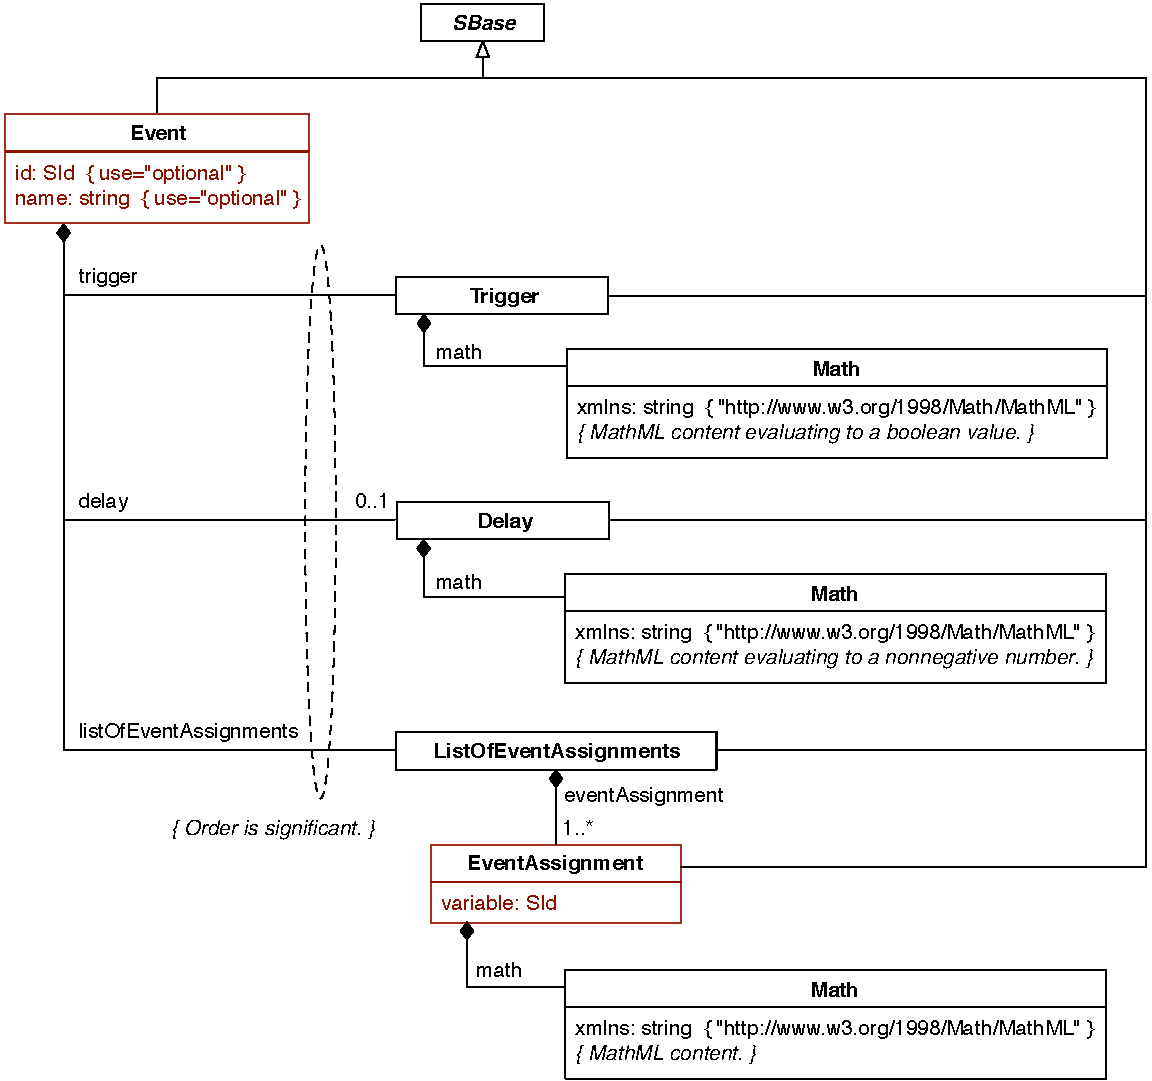
\includegraphics[scale=0.8]{figs/event-uml}
  \caption{\changed{The definitions of \Event, \Trigger, \Delay
      and \EventAssignment, and the container class
      \ListOfEventAssignments.}}
  \label{fig:event}
\end{figure}


\subsubsection{\class{Event}}

An \Event definition has three required parts: an identifier, a
trigger condition and at least one \EventAssignment.  \changed{In
  addition, an event can include an optional delay.  These various
  aspects of \Event are described below.}

\begin{blockChanged}

Previous definitions of \Event in SBML Level~2 included an
additional attribute called \token{timeUnits}, which allowed the
time units of the \Delay to be set explicitly.  \sbmltwothree
removes this attribute for several reasons.  First, the ability to
change the time units of the delay time of an \Event to be
different from the units of time for the whole model meant that
computing an \Event's time of triggering and its delay might have
to be done using two different sets of units---a potential source
of overlooked errors.  Second, the ability to redefine the units
of time for the delay of an \Event became inconsistent with the
lack of such a field on other \sbmltwothree components involving
an element of time, such as \RateRule and \KineticLaw.  On
balance, the \token{timeUnits} feature was judged to add needless
complexity and inconsistency for little gain in functionality.

\end{blockChanged}


\paragraph{The \token{id} and \token{name} \changed{attributes}}
\label{sec:event-id-name}

\begin{blockChanged}

As with most components in SBML, an \Event has \token{id} and
\token{name} attributes, but in the case of \Event, both are optional.
These attributes operate in the manner described in
Section~\ref{sec:idnameattribs}.

\end{blockChanged}


\paragraph{The optional \token{sboTerm} \changed{attribute} on \class{Event}}
\label{sec:event-sboterm}

\changed{As with all SBML components derived from \SBase, an
  \Event has an optional \changed{attribute} \token{sboTerm} of
  type \primtype{SBOTerm} }\changed{ (see
  Sections~\ref{sec:sboterm-type} and~\ref{sec:sboTerm}).}  When a
value is given to this \changed{attribute}, it must be a valid
term derived from \sboevent in SBO.  The \Event should have an
``is a'' relationship with the SBO term, and the term should be
the most precise (narrow) term that captures the meaning of the
event in the model.

As discussed in Section~\ref{sec:sboTerm}, SBO labels are optional
information on a model.  Applications are free to ignore
\token{sboTerm} values.  A model must be interpretable without the
benefit of SBO labels.


\begin{blockChanged}

\subsubsection{\class{Trigger}}
\label{sec:trigger}
\label{sec:event-trigger}

As shown in Figure~\ref{fig:event}, the \token{trigger} \changed{element} of
an \Event must contain exactly one object of class \Trigger.  This
object contains one \token{math} \changed{element} containing a MathML
expression.  The expression must evaluate to a value of type
\primtype{boolean}.  The exact moment at which the expression
evaluates to \val{true} is the time point when the \Event is
\emph{fired}.

\newpage

An event only fires when its \Trigger expression makes the
transition in value from \val{false} to \val{true}.  The event
will also fire at any future time points when the \token{trigger}
make this transition; in other words, an event can fire multiple
times during a simulation if its trigger condition makes the
transition from \val{false} to \val{true} more than once.

An important question is whether an event can fire prior to, or
at, initial simulation time, \ie $t \leq 0$.  The answer is no: an
event can only be triggered immediately after initial simulation
time \ie $t > 0$.


\paragraph{The optional \token{sboTerm} \changed{attribute} on \class{Trigger}}
\label{sec:trigger-sboterm}

As with all SBML components derived from \SBase, \Trigger inherits
the optional \changed{attribute} \token{sboTerm} of type
\primtype{SBOTerm} (see Sections~\ref{sec:sboterm-type}
and~\ref{sec:sboTerm}).  When a value is given to this
\changed{attribute}, it must be a valid term representing a
mathematical expression (\ie a term chosen from the
\sbomathformula hierarchy).  The formula in the \Trigger's
\token{math} expression should have an ``is a'' relationship with
the SBO term, and the term should capture most precise (narrow)
meaning of the mathematical formula of the trigger.


\subsubsection{\class{Delay}}
\label{sec:event-delay}

As shown in Figure~\ref{fig:event}, an \Event object can contain
an optional \token{delay} \changed{element} of class \Delay.  The \Delay is
derived from \SBase and contains a mathematical formula stored in
\token{math}.  The formula is used to compute the length of time
between when the event has \emph{fired} and when the event's
assignments (see below) are actually \emph{executed}.  If no delay
is present on a given \Event, a time delay of zero is assumed.

The expression in \token{math} must be evaluated at the time the
rule is \emph{fired}.  The expression must always evaluate to a
positive number (otherwise, a nonsensical situation could arise
where an event is defined to fire before it is triggered!).  


\paragraph{Units of delay expressions}

The units of the numerical value computed by the delay expression
must be units of time (Section~\ref{sec:built-in-units}).  Note
that units are \emph{not} predefined or assumed for the contents
of \token{math} in a \Delay object; rather, they must be defined
explicitly for each instance of a \Delay object in a model.  This
is an important point to bear in mind when pure numbers are used
in delay expressions.

For example, the following \Event instance would not satisfy the
model consistency rules in SBML described in this specification
and summarized in Appendix~\ref{apdx:validation-rules}): the
expression inside the \token{math} element does not have any
declared units, whereas what is required in this context is units
of time:

\begin{example}
<model>
    ...
    <listOfEvents>
        <event>
            ...
            <delay>
                <math xmlns="http://www.w3.org/1998/Math/MathML">
                    <cn> 1 </cn>
                </math>
            </delay>
            ...
        </event>
    </listOfEvents>
    ...
</model>
\end{example}

The \val{<cn> 1 </cn>} within the mathematical formula of the
\token{delay} above has \emph{no units declared}.  To make the
expression have the needed units of time, we must use one of the
techniques discussed in Section~\ref{sec:units-of-mathml}, namely,
either defining a parameter for the number and using it in place
of the number, or else multiplying the number with a parameter
having the proper units.  Here we employ the second approach as an
illustration:

\begin{example}
<model>
    ...
    <listOfParameters>
        <parameter id="TimeUnits" value="1" units="time"/>
    </listOfParameters>
    ...
    <listOfEvents>
        <event>
            ...
            <delay>
                <math xmlns="http://www.w3.org/1998/Math/MathML">
                    <apply>
                        <times/>
                        <cn> 1 </cn>
                        \changed{<ci> TimeUnits </ci>}
                    </apply>
                </math>
            </delay>
            ...
        </event>
    ...
</model>
\end{example}


\paragraph{The optional \token{sboTerm} \changed{attribute} on \class{Delay}}
\label{sec:delay-sboterm}

As with all SBML components derived from \SBase, \Delay inherits
an optional \token{sboTerm} \changed{attribute} of type \primtype{SBOTerm} (see
Sections~\ref{sec:sboterm-type} and~\ref{sec:sboTerm}).  When a
value is given to this \changed{attribute}, it must be a valid term derived from
the \sbomathformula hierarchy in SBO.  The \Delay formula should
have an ``is a'' relationship with the chosen SBO term, and the
term should be the most precise (narrow) term that captures the
meaning of the delay expression.



\subsubsection{\class{EventAssignment}}
\label{sec:eventassignment}
\label{sec:listofeventassignments}

\Event contains a mandatory element called
\token{listOfEventAssignments}, of class \ListOfEventAssignments.
In every instance of an event definition in a model, the object's
\token{listOfEventAssignments} element must have a non-empty list
of one or more \token{eventAssignment} elements of class
\EventAssignment.  The object class \EventAssignment has one
required attribute, \token{variable}, and a required element,
\token{math}.  Being derived from \SBase, it also has all the
usual attributes and elements of its parent class.

An ``event assignment'' has effect when the event is
\emph{executed}; that is, at the end of any given delay period (if
given) following the moment that the \Event is triggered.  See
Section~\ref{sec:events-semantics} below for more information
about events and event assignments in SBML.

\end{blockChanged}

\paragraph{The \token{variable} \changed{attribute}}

The \token{variable} \changed{attribute} is of type \primtype{SId} and can
contain the identifier of a \Compartment, \Species or \Parameter
instance defined in the model.  When the event fires, the value of
the model component identified by \token{variable} is changed by
the \EventAssignment to the value computed by the \token{math}
\changed{element}; that is, a species' quantity, compartment's size or
parameter's value are reset to the value computed by \token{math}.

Certain restrictions are placed on what can appear in
\token{variable}:
\begin{itemize}
  
\item The object identified by the value of the \token{variable}
  \changed{attribute} must not have its \token{constant} \changed{attribute} set to or default
  to \val{true}.  (Constants cannot be affected by events.)
  
\item The \token{variable} \changed{attribute} must not contain the identifier
  of a reaction; only species, compartment and parameter values
  may be set by an \Event.
  
\item The value of every \token{variable} \changed{attribute} must be unique
  among the set of \EventAssignment \changed{objects} within a given
  \Event \changed{instance}.  In other words, a single event cannot have
  multiple \EventAssignment{}s assigning the same variable.  (All
  of them would be performed at the same time, when that
  particular \Event triggers, resulting in indeterminacy.)
  Separate \Event instances can refer to the same variable.
  
\item A variable cannot be assigned a value in an \EventAssignment
  object instance and also be assigned a value by an
  \AssignmentRule, \ie the value of the \token{variable} attribute
  in an \EventAssignment instance cannot be the same as the value
  of a \token{variable} attribute in a \AssignmentRule instance.
  (Assignment rules hold at all times, therefore it would be
  inconsistent to also define an event that reassigns the value of
  the same variable.)

\end{itemize}


\paragraph{The optional \token{sboTerm} \changed{attribute} on \class{EventAssignment}}
\label{sec:eventassignment-sboterm}

\EventAssignment has an optional \token{sboTerm}
\changed{attribute} of type \primtype{SBOTerm} (see
Sections~\ref{sec:sboterm-type} and~\ref{sec:sboTerm}).  When a
value is given to this \changed{attribute}, it must be a valid SBO term
identifier referring to a mathematical expression (\ie terms
derived from \sbomathformula).  The \EventAssignment should have
an ``is a'' relationship with the SBO term, and the term should be
the most precise (narrow) term that captures the form of the
assignment formula in the model.


\paragraph{\class{EventAssignment}'s \token{math}}

The \token{math} \changed{element} contains a MathML expression that defines
the new value of the variable. This expression is evaluated when
the \Event is \emph{fired} but the variable only acquires the
result or new value when the \Event is \emph{executed}. The order
of the \EventAssignment \changed{objects} is not significant; the effect
of one assignment cannot affect the result of another assignment.
The identifiers occurring in the MathML \token{ci} \changed{attributes} of the
\EventAssignment \changed{object} represent the value of the identifier
at the point when the \Event is \emph{fired}.


\begin{blockChanged}

\paragraph{Units of the \token{math} formula in \class{EventAssignment}}

In all cases, as would be expected, the units of the formula
contained in the \token{math} \changed{element} of
\EventAssignment must be consistent with the units of the object
identified by the \token{variable} \changed{attribute}.  More
precisely:
\begin{itemize}
  
\item \emph{In the case of a species}, an \EventAssignment sets
  the referenced species' quantity (\quantity{concentration} or
  \quantity{amount of substance}) to the value determined by the
  formula in \token{math}.  The units of the \token{math} formula
  must be identical to the \emph{units of the species} as defined
  in Section~\ref{sec:species-units}.
  
\item \emph{In the case of a compartment}, an \EventAssignment
  sets the referenced compartment's size to the size determined by
  the formula in \token{math}.  The overall units of the formula
  must be identical to the units specified for the size of the
  compartment identified by the value of the \EventAssignment's
  \token{variable} \changed{attribute}.  (See
  Section~\ref{sec:compartment-units} for an explanation of how
  the units of the compartment's size are determined.)
  
\item \emph{In the case of a parameter}, an \EventAssignment sets
  the referenced parameter's value to that determined by the
  formula in \token{math}.  The overall units of the formula must
  be identical to the units defined for the parameter identified
  by the value of the \EventAssignment's \token{variable}
  \changed{attribute}.  (See Section~\ref{sec:parameter-units} for
  an explanation of how the units of the parameter are
  determined.)

\end{itemize}

Note that the formula placed in the \token{math} \changed{element}
has no assumed units.  The consistency of the units of the
formula, and the units of the entity which the assignment affects,
must be explicitly established just as in the case of the value of
\token{delay}.  An approach similar to the one discussed in
Section~\ref{sec:event-delay} may be used.

\end{blockChanged}


\subsubsection{Example \class{Event} definitions}

A example of an \Event \changed{object} follows.  This structure makes the
assignment $k_2 = 0$ at the point when $P_1 \leq t$:

\begin{example}
<event>
    ...
    <listOfUnitDefinitions>
        <unitDefinition id="per_second">
            <listOfUnits>
                <unit kind="second" exponent="-1" multiplier="1" offset="0"/>
            </listOfUnits>
        </unitDefinition>
    </listOfUnitDefinitions>
    ...
    <listOfParameters>
        ...
        <parameter id="k2" value="0.05" units="per_second"/>
        <parameter id="PerSecond" value="1" units="per_second"/>
        ...
    </listOfParameters>
    ...
    <listOfEvents>
        <event>
            <trigger>
                <math xmlns="http://www.w3.org/1998/Math/MathML">
                    <apply>
                        <leq/>
                        <ci> P1 </ci>
                        <ci> t </ci>
                    </apply>
                </math>
            </trigger>
            <listOfEventAssignments>
                <eventAssignment variable="k2">
                    <math xmlns="http://www.w3.org/1998/Math/MathML">
                        <apply>
                            <times/>
                            <cn> 0 </cn>
                            <ci> PerSecond </cn>
                        </apply>
                    </math>
                </eventAssignment>
            <listOfEventAssignments>
        </event>
    </listOfEvents>
    ...
</model>
\end{example}

A complete example of a model using events is given in
Section~\ref{sec:eventeg}.


\subsubsection{Detailed semantics of events}
\label{sec:events-semantics}

The description of events above describes the action of events in
isolation from each other.  This section describes how events
interact.

Events whose \token{trigger} expression is true at the start of a
simulation do not \emph{fire} at the start of the simulation ($t =
0$).  Events \emph{fire} only when the trigger \emph{becomes}
true, \ie the trigger expression transitions from false to true,
which cannot happen at $t = 0$ but can happen at $t > 0$.

Any transition of a \token{trigger} expression from \val{false} to
\val{true} will cause an \token{event} to \emph{fire}.  Consider
an \token{event} $E$ with delay $d$ where the \token{trigger}
expression makes a transition from false to true at times $t_1$
and $t_2$.  The \EventAssignment \changed{object} will have effect at
$t_1+d$ and $t_2+d$ irrespective of the relative times of $t_1$
and $t_2$. For example events can ``overlap'' so that $t_1 < t_2 <
t_1+d$ still causes an event assignments to occur at $t_1+d$ and
$t_2+d$.

It is possible for events to \emph{fire} other events, \ie an
event assignment can cause an event to \emph{fire}, therefore it
is possible for a model to be entirely encoded in \Event
\changed{objects}.

It is entirely possible for two events to be \emph{executed}
simultaneously in simulated time.  It is assumed that, although
the precise time at which these events are \emph{executed} is not
resolved beyond the given point in simulated time, the order in
which the events occur is resolved.  This order can be significant
in determining the overall outcome of a given simulation. SBML
Level 2 does not define the algorithm for determining this order
(the tie-breaking algorithm).  As a result, the results of
simulations involving events may vary when simultaneous events
occur during simulation.  It is anticipated that future versions
or levels of SBML will define a specific set of tie-breaking
algorithms and a mechanism for models to indicate which algorithm
should be applied during simulation.

Despite the absence of a specific tie-breaking algorithm, SBML
event simulation is constrained as follows. When an event $X$
\emph{fires} another event $Y$ and event $Y$ has zero delay then
event $Y$ is added to the existing set of simultaneous events that
are pending \emph{execution}.  Events such as $Y$ do not have a
special priority or ordering within the tie-breaking algorithm.
Events $X$ and $Y$ form a cascade of events at the same point in
simulation time.  All events in a model are open to being in a
cascade.  The position of an event in the event list does not
affect whether it can be in the cascade: $Y$ can be triggered
whether it is before or after $X$ in the list of events.  A
cascade of events can be infinite (never terminate).  When this
occurs a simulator should indicate this has occurred, i.e. it is
incorrect for the simulator to arbitrarily break the cascade and
continue the simulation without at least indicating the infinite
cascade occurred. A variable can change more than once when
processing simultaneous events at simulation time $t$.  The model
behavior (output) for such a variable is the value of the variable
at the end of processing all the simultaneous events at time $t$.











% -----------------------------------------------------------------------------
% chunks of text that maybe will be useful some day:
% -----------------------------------------------------------------------------

% Here it pays to reflect more carefully about what a reaction is.
% A reaction represents a process occuring over time.  the process
% acts on the reactants, transforming them in some way into the
% products.  the transformation may be anything from a change in
% the nature of the reactants to a simple relocation without any
% change to the nature of the reactants; for the purpose of talking
% about the speed of the reaction it does not matter.

% The ``kinetic law'' is a statement about the speed at which the
% process takes place, or more precisely, the frequency of the
% events occuring in this process.  It is by default in terms of
% moles per second, which has some intuitive appeal when dealing
% with chemical substances.  But notice that a ``mole'' is actually
% a statement about numbers of ``things'': it is 6.02e23 of whatever
% is involved.  In the case of chemical species, it is molecules of
% the substance.  To say ``one mole of'' is a shorthand way of
% saying ``6.02e23 molecules of''.  Thus, a reaction expressed as
% ``X moles per second'' is a statement that the process involves
% ``(X times 6.02e23) items per second''.

% 1 kg/sec is 1 kg/sec

% If in a reaction, the units of the species are the same as the
% reaction's substance units (default mole, redefinable by
% redefining ``substance''; sec section x), then the stoichiometries
% represent simply the ratios of the participating species: 1 mole
% of this to 2 moles of that, and so on.  If instead the species are
% given in different units, then the species quantities must be
% converted to be consistent with the units of the reaction.  Thus,
% the SBML stoichiometry may then have to incorporate a conversion:
% the stoichiometry will represent the product of the biochemical
% reaction stoichiometry and a ratio between the species substance
% and the reaction substance.

% don't forget units of reaction id


% ---

% started trying to generate the event diagram in pgf but
% it's too hard.

%   \begin{tikzpicture}[level distance=2in]
%     \node[left=1.15in,above=0.35in] (a) { \emptyClassbox{\textsl{SBase}} };
%     \node[left=0.75in] (b) {
%       \begin{classbox}{Event}
%         id: SId  \{ use="optional" \}     \\
%         name: string \{ use="optional" \} \\
%       \end{classbox} 
%     }
%     [diamond-,edge from parent fork right,grow=right,sibling distance=0.6in]
%     child {node[right=0.15in] (c) { \emptyClassbox{ListOfEventAssignments} }
%       child {node (f) {
%           \begin{classbox}{EventAssignment}
%             variable: SId                                                   \\
%           \end{classbox}
%         }}
%       child {node (g) {
%           \begin{classbox}{Math}
%             xmlns: string \{ "http://www.w3.org/1998/Math/MathML" \} \\
%             \{ \emph{\mathml content} \} \\
%           \end{classbox}
%         }}
%     }
%     child {node[right=0.15in] (d) { \emptyClassbox{Delay} }
%     }
%     child {node[right=0.15in] (d) { \emptyClassbox{Trigger} }
%     }
      
% junk

%      [diamond-,edge from parent fork down,sibling distance=0.6in]
%         \begin{classbox}{Delay}
%           xmlns: string \{ "http://www.w3.org/1998/Math/MathML" \} \\
%           \{ \emph{\mathml content} \} \\
%         \end{classbox}
%       }}
%     child {node[right=0.15in] (e) {
%         \begin{classbox}{Trigger}
%           xmlns: string \{ "http://www.w3.org/1998/Math/MathML" \} \\
%           \{ \emph{\mathml content evaluating to a boolean value} \} \\
%         \end{classbox}
%       }}
%    ;
%           \begin{classbox}{EventAssignment}
%             variable: SId                                                   \\
%             math: Math \{ namespace="http://www.w3.org/1998/Math/MathML" \} \\
%           \end{classbox}
%      \draw[open triangle 60-] (a) -- (b);
%      \draw node[left=0.4in,above=0.375in] {\textsf{math}};
%      \draw node[left=0.3in,below=0.225in] {\textsf{message}};
%      \draw node[left=-0.15in,below=0.215in] {\textsf{0..1}};
%  \end{tikzpicture}

%   \begin{blockChanged}
%   \vspace*{2ex}
%   \begin{classbox}{Trigger}
%     math: Math \{ namespace="http://www.w3.org/1998/Math/MathML" \} \\
%   \end{classbox}
%   \vspace*{2ex}
%   \begin{classbox}{Delay}
%     math: Math \{ namespace="http://www.w3.org/1998/Math/MathML" \} \\
%   \end{classbox}
%   \vspace*{2ex}
%   \end{blockChanged}
